\chapter{Kerr black hole}
\label{s:ker}
\index{Kerr!black hole}

\minitoc

\section{Introduction}

Having studied the Schwarzschild black hole in the preceding
chapters, we turn now to its rotating generalization: the Kerr black hole.
The Kerr metric is arguably the most important solution of general relativity,
largely because of the no-hair theorem, according to which
all stationary black holes in the Universe are Kerr black holes (cf. Sec.~\ref{s:sta:no-hair}).

In this chapter, the Kerr solution is first presented in terms of
the standard Boyer-Lindquist coordinates and its basic properties are
discussed (Sec.~\ref{s:ker:Kerr_solution}). Then Kerr coordinates are introduced
in Sec.~\ref{s:ker:extension}; contrary to Boyer-Lindquist coordinates,
they are regular on the two Killing horizons of Kerr spacetime.
Kerr coordinates are also tied to one of the two congruences of
null geodesics related to the spacetime conformal structure: the
principal null geodesics, which are introduced in Sec.~\ref{s:ker:principal_geod}.
The second congruence, that of the so-called \emph{outgoing} principal null geodesics,
provides the generators of the black hole event horizon, which is
studied in Sec.~\ref{s:ker:event_hor_gen}.
Then Sec.~\ref{s:ker:global_quantities}
focuses on global quantities characterizing Kerr spacetime: mass, angular
momentum and horizon area.
Section~\ref{s:ker:observers} presents various standard families of observers in
Kerr spacetime.
Finally, Sec.~\ref{s:ker:max_extension} discusses the maximal analytical extension of Kerr spacetime
and the concept of Cauchy horizon.


\section{The Kerr solution} \label{s:ker:Kerr_solution}

\subsection{Expression in Boyer-Lindquist coordinates} \label{s:ker:expr_BL}

The Kerr solution depends on two constant non-negative real parameters:
\begin{itemize}
\item the \defin{mass parameter}\index{mass!parameter of Kerr solution} $m > 0$, to be
interpreted in Sec.~\ref{s:ker:Komar_mass} as the spacetime total mass;
\item the \defin{spin parameter}\index{spin!parameter of Kerr solution} $a \geq 0 $,
to be interpreted in Sec.~\ref{s:ker:Komar_J} as the reduced angular momentum  $a=J/m$, $J$ being the
spacetime total angular momentum.
\end{itemize}
In this chapter, we focus on Kerr solutions for which
\be \label{e:ker:a_lower_m}
    0 < a < m ,
\ee
postponing the case $a=m$ to Chap.~\ref{s:exk}.
The Kerr solution is usually presented in the so-called
\defin{Boyer-Lindquist coordinates}\index{Boyer-Lindquist coordinates}
$(t,r,\th,\ph)$. Except for the standard singularities of the
spherical coordinates $(\th,\ph)$ on $\SS^2$ at $\theta\in\{0,\pi\}$,
we may consider that Boyer-Lindquist coordinates cover the manifold
$\R^2\times\SS^2$, with $t$ spanning $\R$, $r$
spanning\footnote{This contrasts with $r$ spanning only $(0,+\infty)$ for
the standard spherical coordinates $(r,\th,\ph)$ on $\R^3$.} $\R$,
$\th$ spanning $(0,\pi)$ and $\ph$ spanning $(0,2\pi)$. Hence
$(t,r)$ is a Cartesian chart covering $\R^2$ and $(\th,\ph)$ is the standard
spherical chart of $\SS^2$.

\begin{figure}
\centerline{\includegraphics[width=0.8\textwidth]{ker_spher_view.pdf}}
\caption[]{\label{f:ker:spher_view} \footnotesize
View of a section $t=\mathrm{const}$ of $\mathbb{R}^2\times\mathbb{S}^2$
in terms of the coordinates $(R,\th,\ph)$, with $R:=\mathrm{e}^r$,
so that the region $r\rightarrow -\infty$
is reduced to a single point at the centre of all the pictured spheres.
Such coordinates have been introduced for pictorial purposes by O'Neill\index{O'Neill!coordinates}
\cite{ONeil95}.}
\end{figure}


In this section, we choose the spacetime manifold to be the open subset $\M_{\rm BL}$
of $\R^2\times\SS^2$ formed by the disjoint union of
the following three connected components (cf. Fig.~\ref{f:ker:spher_view}):
\begin{subequations}
\begin{align}
    \M_{\rm BL} & :=  \M_{\rm I} \cup \M_{\rm II} \cup \M_{\rm III} , \label{e:ker:def_M_BL} \\
    \M_{\rm I} & :=  \R\times(r_+,+\infty)\times\SS^2 \label{e:ker:def_M_I}\\
    \M_{\rm II} & :=  \R\times(r_-,r_+)\times\SS^2 \\
    \M_{\rm III} & :=  \R\times(-\infty,r_-)\times\SS^2 \setminus \ring, \label{e:ker:def_M_III}
\end{align}
\end{subequations}
where
\be \label{e:ker:def_r_pm}
    \encadre{r_+ := m + \sqrt{m^2-a^2}} \quad\mbox{and}\quad  \encadre{r_- := m - \sqrt{m^2-a^2}}
\ee
and $\ring$ is the subset of $\R^2\times\SS^2$ defined in terms of Boyer-Lindquist coordinates $(t,r,\th,\ph)$ by
\be \label{e:ker:def_ring}
    \ring := \left\{ p \in \R^2\times\SS^2,
        \quad r(p) = 0 \ \mbox{and}\ \th(p) = \frac{\pi}{2} \right\} .
\ee
\begin{remark}
By construction, the points of $\R^2\times\SS^2$ obeying $r=r_-$ and $r=r_+$ are
excluded from the spacetime manifold $\M_{\rm BL}$. In a latter stage
(Sec.~\ref{s:ker:extension}), we shall extend the spacetime manifold to
include these points, so that the spacetime manifold will be $\M = \R^2\times\SS^2\setminus \ring$. Even latter on, after having noticed that $(\M,\w{g})$ is not geodesically complete,
we shall extend the spacetime manifold further and discuss the maximal analytic
extension (Sec.~\ref{s:ker:max_extension}).
\end{remark}

\begin{remark} \label{r:ker:r_zero}
One shall stress that the points having $r=0$ are \emph{not} special points in
$\R^2\times\SS^2$ spanned by the coordinates $(t,r,\th,\ph)$. In particular,
$(t,r) = (t_0, 0)$, where $t_0$ is a constant, defines a regular sphere
$\Sp_0$ diffeomorphic to $\SS^2$. On the spacetime manifold $\M_{\rm BL}$, the
points $r=0$ are part of $\M_{\rm III}$ and because of the exclusion of $\ring$
in the definition (\ref{e:ker:def_M_III}), $(t,r) = (t_0, 0)$ defines
a sphere minus its equator (cf. Fig.~\ref{f:ker:spher_view}, where the equator
is the tick orange circle).
\end{remark}

Note that thanks to the constraint (\ref{e:ker:a_lower_m}), $r_+$ and $r_-$
are well-defined and obey
\be \label{e:ker:order_r_pm}
    0 < r_- < m < r_+ < 2 m .
\ee
Note also that $\ring$ is spanned by the coordinates $(t,\ph)$ and is diffeomorphic to the 2-dimensional cylinder $\R\times\SS^1$:
\be \label{e:ker:ring_R_S1}
    \ring \simeq \R\times\SS^1 .
\ee
This is so because $r=0$ is \emph{not} a peculiar value of $r$ in $\R^2\times\SS^2$
(cf. Remark~\ref{r:ker:r_zero} above).
In view of Eqs.~(\ref{e:ker:def_M_I})-(\ref{e:ker:def_M_III}) and (\ref{e:ker:def_ring}), it is clear that
the various connected components of $\M_{\rm BL}$ are defined in terms of
the Boyer-Lindquist coordinates $(t,r,\th,\ph)$ by
\begin{subequations}
\label{e:ker:M_I_III_r}
\begin{align}
  \forall p \in  \M_{\rm BL},\quad p \in \M_{\rm I} & \iff r(p) > r_+ \\
    \quad p \in \M_{\rm II} & \iff r_- < r(p) < r_+ \\
    \quad p \in \M_{\rm III} & \iff r(p) < r_-\ \mbox{and}\
    \left( r(p) \not=0 \ \mbox{or}\ \theta(p) \not=\frac{\pi}{2} \right) .
\end{align}
\end{subequations}

\begin{greybox}
The \defin{Kerr metric}\index{Kerr!metric} is defined
in terms of the Boyer-Lindquist coordinates $(t,r,\th,\ph)$
by
\be \label{e:ker:metric_BL}
    \encadre{
    \begin{array}{ll}
    \w{g}  = &
    \displaystyle - \left( 1 - \frac{2m r}{\rho^2} \right) \, \dd t^2
    - \frac{4 a m  r \sin^2\th}{\rho^2} \,  \dd t\, \dd\ph
    + \frac{\rho^2}{\Delta} \, \dd r^2  \\[2ex]
    & \displaystyle + \rho^2 \dd \th^2
    + \left( r^2 + a^2 + \frac{2 a^2 m r \sin^2\th}{\rho^2} \right)
    \sin^2\th \, \dd \ph^2 ,
    \end{array}
    }
\ee
with
\be \label{e:ker:def_rho2}
    \encadre{\rho^2 := r^2 + a^2 \cos^2\th}
\ee
and
\be \label{e:ker:def_Delta}
    \encadre{\Delta := r^2 - 2 m r + a^2 = (r-r_-)(r-r_+)} .
\ee
\end{greybox}

Note that on $\M_{\rm BL}$, $\rho\not=0$ and $\Delta\not=0$ (by construction
of $\M_{\rm BL}$!), so that the metric components (\ref{e:ker:metric_BL})
are regular in $\M_{\rm BL}$, except for the standard singularities of
the spherical coordinates $(\th,\ph)$.

By means of a computer algebra system (cf. the SageMath notebook~\ref{s:sam:Kerr_solution}),
one checks easily:
\begin{prop}[Kerr metric as a solution of the vacuum Einstein equation]
The Kerr metric $\w{g}$ [Eq.~(\ref{e:ker:metric_BL})] is a solution of the vacuum
Einstein equation\index{Einstein!equation!vacuum --}\index{vacuum!Einstein equation}
(\ref{e:fra:vac_Einstein}) on $\M_{\rm BL}$.
\end{prop}

\begin{hist}
\label{h:ker:Kerr_sol}
The Kerr solution has been found by the New Zealand mathematician Roy P. Kerr\index[pers]{Kerr, R.P.} (then at the University of Texas at Austin) in the spring of 1963
\cite{Kerr63}. Kerr was searching for \emph{algebraically special}\index{algebraically special metric} metrics, i.e. metrics whose Weyl conformal curvature
tensor admits a \emph{doubly degenerate principal null direction} (to be defined
in Sec.~\ref{s:ker:principal_geod} below), in the case where the
principal null congruence has a non-vanishing twist (or ``rotation''). The special case of vanishing twist (i.e. hypersurface-orthogonal
congruence) had been treated by Ivor Robinson\index[pers]{Robinson, I.} and
Andrzej Trautman\index[pers]{Trautman, A.} in 1962 \cite{RobinT62}.
Kerr used
Cartan's structure equations\index{Cartan!structure equations} in a null tetrad
to manipulate the Einstein equation; he obtained the solution in coordinates different from the Boyer-Lindquist ones, known today as \emph{Kerr coordinates} and
to be discussed in Sec.~\ref{s:ker:Kerr_coord} (cf. the historical note page~\pageref{h:ker:Kerr_coord}). For more details about this fantastic discovery, see the
account by Kerr himself in Refs.~\cite{Kerr09,KrasiVK09}.
Boyer-Lindquist coordinates have been introduced in 1966 by Robert H.~Boyer\index[pers]{Boyer, R.H.} (see the historical note on p.~\pageref{h:sta:Boyer}) and Richard W. Lindquist\index[pers]{Lindquist, R.W.} \cite{BoyerL67} (compare Eq.~(2.13) of Ref.~\cite{BoyerL67} with
Eq.~(\ref{e:ker:metric_BL}) above, keeping in mind that Boyer and Lindquist used
$-a$ instead of $a$, following Kerr's convention in the discovery article~\cite{Kerr63}, cf.
the historical note on p.~\pageref{h:ker:Kerr_coord}).
\end{hist}

\subsection{Basic properties} \label{s:ker:basic_prop}

Various properties of the Kerr metric are immediate:

\begin{prop}[asymptotic flatness of Kerr spacetime]
The spacetime $(\M_{\rm BL},\w{g})$ has two asymptotically flat ends: one in
$\M_{\rm I}$ for $r\rightarrow + \infty$, which is equivalent to the asymptotics
of a Schwarzschild spacetime of mass $m$ and the other one
in $\M_{\rm III}$ for $r\rightarrow - \infty$, which is equivalent to
the asymptotics of a Schwarzschild spacetime of (negative!) mass $-m$.
\end{prop}

\begin{proof}
For $r\rightarrow+\infty$ or $r\rightarrow-\infty$, one has $\rho^2\sim r^2$ and
$\rho^2/\Delta \sim (1-2m/r)^{-1}$,
and $4 a m  r / \rho^2\,  \dd t\, \dd\ph \sim 4 a m/r^2 \,  \dd t\, r\dd\ph$,
so that the metric (\ref{e:ker:metric_BL}) becomes
\be \label{e:ker:asympt_metric}
    \w{g}  \simeq  - \left( 1 - \frac{2m}{r} \right) \, \dd t^2
    + \left( 1 - \frac{2m}{r} \right) ^{-1} \dd r^2
    + r^2 \left( \dd \th^2 + \sin^2\th  \, \dd \ph^2 \right)
    + O\left(\frac{1}{r^2}\right)
\ee
For $r>0$, we recognize the Schwarzschild metric\index{Schwarzschild!metric} expressed
in Schwarzschild-Droste coordinates [Eq.~(\ref{e:sch:Schwarz_metric_SD})].
For $r<0$, the change of coordinate $r'=-r$ leads to the Schwarzschild metric
as well, but with the negative mass parameter $m'=-m$.
\end{proof}

\begin{prop}[stationarity and axisymmetry of Kerr spacetime]
The spacetime $(\M_{\rm BL},\w{g})$ admits two isometries:
stationarity and axisymmetry, generated respectively by the Killing
vectors
\be \label{e:ker:def_xi_eta}
    \encadre{\w{\xi} := \wpar_t} \quad\mbox{and}\quad
    \encadre{\w{\eta} := \wpar_\ph}.
\ee
\end{prop}
\begin{proof}
All the metric components $g_{\alpha\beta}$ in Eq.~(\ref{e:ker:metric_BL})
are independent from $t$ and $\ph$. This implies that the vector fields (\ref{e:ker:def_xi_eta}) are Killing vectors (cf. Sec.~\ref{s:neh:symmetries}).
Since $t$ spans $\R$, the isometry group generated by $\w{\xi}$ is clearly
the translation group\index{translation!group}\index{group!translation --} $(\R,+)$. Moreover, in
view of (\ref{e:ker:asympt_metric}), we have $\w{\xi}\cdot\w{\xi} = g_{tt} < 0$
as $r\rightarrow +\infty$, which means that the Killing vector $\w{\xi}$
is asymptotically timelike. Given the definition of stationarity stated in
Sec.~\ref{s:sta:def_station}, we conclude that the Kerr spacetime is
stationary.
On the other side, since $\ph$ is an azimuthal coordinate
on $\SS^2$, the isometry group generated by $\w{\eta}$ is the rotation
group\index{rotation!group}\index{group!rotation --} $\mathrm{SO}(2) = \mathrm{U}(1)$.
Moreover, $\wpar_\ph$ is spacelike for $r\to +\infty$ (even for $r>0$).
Hence, the Kerr spacetime is axisymmetric (cf. the definition given in Sec.~\ref{s:sta:Komar_angu_mom}).
\end{proof}

\begin{prop}[non-staticity for $a\neq 0$]
For $a\neq 0$, as we have assumed in (\ref{e:ker:a_lower_m}), the
Kerr spacetime is not static (cf. the definition in Sec.~\ref{s:sta:def_station}):
the stationary Killing vector $\w{\xi}$ is not hypersurface-orthogonal.
\end{prop}

\begin{proof}
From Eq.~(\ref{e:ker:metric_BL}), we have
$\w{\xi}\cdot\w{\eta} = g_{t\ph} \neq 0$ for $a\neq 0$.
Since $\w{\eta}=\wpar_\ph$ is tangent to the hypersurfaces $t=\mathrm{const}$, this implies
that $\w{\xi}$ is not normal to these hypersurfaces.
That there does not exist any hypersurface
family orthogonal to $\w{\xi}$ can be seen from the non-vanishing of the twist 3-form\index{twist 3-form} defined by Eq.~(\ref{e:neh:def_twist_3form}):
$\w{\omega} := \uu{\xi}\wedge \dd\uu{\xi}$. We have indeed (see the notebook~\ref{s:sam:Kerr_solution} for the computation)
\[
    \w{\omega} = \frac{2 a m \sin\th}{\rho^4} \Big[
        \sin\th (a^2\cos^2\th - r^2) \, \dd t \wedge \dd r \wedge \dd \ph
        + 2 \Delta r \cos\th \, \dd t \wedge \dd \th \wedge \dd \ph \Big] .
\]
Clearly $\w{\omega} \neq 0$ as soon as $a\neq 0$. According to the
Frobenius theorem\index{Frobenius!theorem} (see e.g.
Eq.~(B.3.6) in Wald's textbook \cite{Wald84}), it follows that
$\w{\xi}$ is not hypersurface-orthogonal.
\end{proof}

\begin{prop}[Schwarzschild limit]
For $a\to 0$, the Kerr metric reduces to the Schwarzschild metric.
\end{prop}

\begin{proof}
When $a\rightarrow 0$, we have $r_+\rightarrow 2m$, $r_-\rightarrow 0$,
$\rho^2\sim r^2$, and $\rho^2/\Delta \sim (1-2m/r)^{-1}$, and we see on
(\ref{e:ker:metric_BL}) that the Kerr metric reduces to the Schwarzschild metric
expressed
in Schwarzschild-Droste coordinates [Eq.~(\ref{e:sch:Schwarz_metric_SD})].
\end{proof}

\begin{prop}[the double flat disk at $r=0$]
The metric induced by the Kerr metric on the hypersurface $r=0$ of $\M_{\rm BL}$
is
\be \label{e:ker:metric_r0}
    \w{h} = - \dd t^2 + a^2\left( \cos^2\th \,  \dd \th^2 + \sin^2\th \, \dd \ph^2 \right) .
\ee
For $a\neq 0$, $\w{h}$ is a flat Lorentzian metric, which can be brought to a
manifestly Minkowskian form via the change coordinates  $x:=a\sin\th\cos\ph$, $y:=a\sin\th\sin\ph$:
$\w{h} = - \dd t^2 + \dd x^2 + \dd y^2$. In particular, for a fixed value
of $t$, the $r=0$ subset
\be \label{e:ker:S_r_zero}
    \mathcal{S}_{0,t} := \{p\in \M_{\rm III}, r(p)=0, t(p)=t\}
\ee
is made of two connected components, which are two \emph{flat open disks} of radius $a$, corresponding respectively to $\theta < \pi/2$ and $\theta>\pi/2$, since
the equator $\theta=\pi/2$ is excluded by the very definition of $\M_{\rm III}$
(cf. Remark~\ref{r:ker:r_zero} above).
\end{prop}
\begin{proof}
On the hypersurface $r=0$, we have $\rho^2=a^2\cos^2\th$, $\Delta=a^2$ and $\dd r = 0$,
so that the Kerr metric (\ref{e:ker:metric_BL}) induces the metric (\ref{e:ker:metric_r0}).
That $\mathcal{S}_{0,t}$ is made of two disks is obvious from the range of
variation of the coordinates $(x,y)$, which by construction obey
$x^2 + y^2 < a^2$ (cf. Fig.~\ref{f:ksm:rzero_disk} in Appendix~\ref{s:ksm},
where the Kerr-Schild coordinates $(x,y)$ coincide with the current coordinates
$(x,y)$, up to some rotation).
\end{proof}

The set $\mathcal{S}_{0,t}$ is depicted
by the dotted red line in Fig.~\ref{f:ker:spher_view}. It is also depicted
in terms of the so-called Kerr-Schild coordinates in
Figs.~\ref{f:ksm:phi_cut} - \ref{f:ksm:2_sheets} of Appendix~\ref{s:ksm}.


\subsection{Determinant and inverse metric}

The determinant of the metric $\w{g}$ with respect to Boyer-Lindquist coordinates
is deduced from (\ref{e:ker:metric_BL}); it takes a
relatively simple form (see the notebook~\ref{s:sam:Kerr_solution} for the computation):
\be
    \det (g_{\alpha\beta}) = - \rho^4 \sin^2\th .
\ee

The inverse metric is (see the notebook~\ref{s:sam:Kerr_solution} for the computation)
\be \label{e:ker:inv_met_BL}
    g^{\alpha\beta} = \left(
    \begin{array}{cccc}
    - \frac{1}{\Delta}
    \left( r^2 + a^2 + \frac{2 a^2 m r \sin^2\th}{\rho^2} \right)
     & 0 & 0 & -\frac{2 a m r}{\rho^2 \Delta} \\[1ex]
    0 & \frac{\Delta}{\rho^2} & 0 & 0 \\[1ex]
    0 & 0 &\frac{1}{\rho^2} & 0 \\[1ex]
    -\frac{2 a m r}{\rho^2 \Delta} & 0 & 0 &
    \frac{1}{\Delta\sin^2\th}\left(1 - \frac{2 m r}{\rho^2} \right)
    \end{array}
    \right) .
\ee


\subsection{Ergoregion} \label{s:ker:ergoregion}

Let us investigate the causal character of the stationary Killing vector $\w{\xi}$.
We have, according to (\ref{e:ker:metric_BL}) and (\ref{e:ker:def_rho2}),
\[
    \w{\xi}\cdot\w{\xi} = g_{tt} = - 1 + \frac{2m r}{r^2 + a^2\cos^2\th} .
\]
Thus
\[
    \w{\xi}\ \mbox{timelike} \iff r^2 - 2 m r + a^2\cos^2\th > 0
        \iff r < r_{\E^-}(\theta) \quad\mbox{or}\quad  r > r_{\E^+}(\theta) ,
\]
with
\be \label{e:ker:ergosphere_radius}
    \encadre{ r_{\E^\pm}(\theta) := m \pm \sqrt{m^2 - a^2\cos^2\th} } .
\ee
Comparing with (\ref{e:ker:def_r_pm}), we note that
\be
    0 \leq r_{\E^-}(\theta) \leq r_- \leq m \leq r_+ \leq r_{\E^+}(\theta)
        \leq 2 m ,
\ee
with
\begin{subequations}
\begin{align}
 & r_{\E^-}(0)  = r_{\E^-}(\pi) = r_- \qand r_{\E^-}(\pi/2) = 0     \label{e:ker:r_ergo_m_eq}  \\
 & r_{\E^+}(0)  = r_{\E^+}(\pi) = r_+ \qand r_{\E^+}(\pi/2) = 2 m . \label{e:ker:r_ergo_p_eq}
\end{align}
\end{subequations}

\begin{figure}
\centerline{\includegraphics[width=0.8\textwidth]{ker_ergo_a90.pdf}}
\caption[]{\label{f:ker:ergo_a90} \footnotesize
Meridional view of a section $t=\mathrm{const}$ of Kerr spacetime with $a/m=0.90$ in
O'Neill exponential coordinates\index{O'Neill!coordinates} $x = \mathrm{e}^{r/m}\sin\th$ and $z = \mathrm{e}^{r/m}\cos\th$ (cf. Fig.~\ref{f:ker:spher_view}).
The right (resp. left) half of the figure corresponds to $\ph=0$ (resp. $\ph=\pi$).
The Roman numbers I, II, III denote the components $\M_{\rm I}$, $\M_{\rm II}$ and
$\M_{\rm III}$ of the manifold $\M_{\rm BL}$. The dotted orange circle marks the location
of $r=0$, while the small black circle at the center of the figure corresponds to
$r\rightarrow -\infty$. The two red dots marks the curvature singularity $\mathscr{R}$.
The ergoregion (cf. Sec.~\ref{s:ker:ergoregion}) is shown in grey, while the
yellow part is Carter time machine (cf. Sec.~\ref{s:ker:time_machine}).
}
\end{figure}

\begin{figure}
\centerline{\includegraphics[width=0.6\textwidth]{ker_ergo_a50.pdf}}
\caption[]{\label{f:ker:ergo_a50} \footnotesize
Same as Fig.~\ref{f:ker:ergo_a90} but for $a/m=0.50$.
}
\end{figure}

\begin{figure}
\centerline{\includegraphics[width=0.8\textwidth]{ker_ergo_a99.pdf}}
\caption[]{\label{f:ker:ergo_a99} \footnotesize
Same as Fig.~\ref{f:ker:ergo_a90} but for $a/m=0.99$.
}
\end{figure}

Given the definition of $\M_{\rm I}$, $\M_{\rm II}$ and $\M_{\rm III}$, we conclude that:

\begin{prop}[ergoregion of Kerr spacetime]
The stationary Killing vector $\w{\xi}$ of Kerr spacetime obeys:
\begin{itemize}
\item $\w{\xi}$ is timelike in the region of $\M_{\rm I}$ defined by $r>r_{\E^+}(\theta)$
and in the region of $\M_{\rm III}$ defined by $r<r_{\E^-}(\theta)$;
\item $\w{\xi}$ is null on the hypersurface $\E^+$ of $\M_{\rm I}$ defined by
$r=r_{\E^+}(\theta)$
and on the hypersurface $\E^-$ of $\M_{\rm III}$ defined by $r=r_{\E^-}(\theta)$;
\item $\w{\xi}$ is spacelike in all $\M_{\rm II}$ and in the region
$\mathscr{G}^+$ of $\M_{\rm I}$
defined by $r<r_{\E^+}(\theta)$, as well as
in the region $\mathscr{G}^-$ of $\M_{\rm III}$ defined by $r>r_{\E^-}(\theta)$.
\end{itemize}
According to the nomenclature introduced in Sec.~\ref{s:sta:strong_rigidity},
one calls $\E^+$ (resp. $\E^-$) the
\defin{outer ergosphere}\index{outer!ergosphere}\index{ergosphere!outer --}
(resp. \defin{inner ergosphere}\index{inner!ergosphere}\index{ergosphere!inner --})
and $\mathscr{G}^+$ (resp. $\mathscr{G}^-$) the
\defin{outer ergoregion}\index{outer!ergoregion}\index{ergoregion!outer --}
(resp. \defin{inner ergoregion}\index{inner!ergoregion}\index{ergoregion!inner --}).
The part of $\M_{\rm BL}$ where $\w{\xi}$ is spacelike, i.e.
$\mathscr{G} = \mathscr{G}^+ \cup \M_{\rm II} \cup \mathscr{G}^-$,
is called the \defin{ergoregion}\index{ergoregion!of Kerr spacetime}.
\end{prop}


Following the standard notation in topology, we shall denote
by $\overline{\mathscr{G}}$ the closure of $\mathscr{G}$, i.e. the
union of the ergoregion and the two ergospheres:
\be
    \overline{\mathscr{G}} := \mathscr{G} \cup \E^- \cup \E^+ .
\ee
The locus where the Killing vector $\w{\xi}$ is timelike is then
$\M_{\rm BL}\setminus \overline{\mathscr{G}}$.

The ergoregion is depicted in Figs.~\ref{f:ker:ergo_a90}--\ref{f:ker:ergo_a99}.
It is worth noticing that
the location of the inner and outer ergospheres in the equatorial
plane ($\th=\pi/2$) do not depend on the spin parameter $a$:
$r_{\E^-}(\pi/2) = 0$ [Eq.~(\ref{e:ker:r_ergo_m_eq})] and
$r_{\E^+}(\pi/2) = 2m$ [Eq.~(\ref{e:ker:r_ergo_p_eq})], a feature
that appears clearly in Figs.~\ref{f:ker:ergo_a90}--\ref{f:ker:ergo_a99},
given that $\mathrm{e}^2 \simeq 7.39$.

\begin{remark} \label{r:ker:static_limit}
Sometimes the word \defin{ergosurface}\index{ergosurface} is used instead of
\emph{ergosphere}. One may encounter as well the names
\emph{infinite redshift surface}\index{infinite redshift surface}\index{redshift!infinite -- surface} (e.g. \cite{Vishv68}) and
\emph{static limit}\index{static!limit} (cf. Sec.~\ref{s:ker:static_obs} below)
for \emph{ergosphere}, especially in old texts.
\end{remark}

\begin{remark}
By construction, the Killing vector $\w{\xi}$ is null on the
ergospheres $\E^+$ and $\E^-$. It is moreover tangent to these
hypersurfaces (see below). However, for $a\neq 0$,
$\E^+$ and $\E^-$ are \emph{not} Killing horizons, as defined
in Sec.~\ref{s:neh:def_Killing_hor}, since
$\w{\xi}$ fails to be normal to them, or equivalently, $\E^+$ and $\E^-$
are not null hypersurfaces. They are actually timelike hypersurfaces,
except on the rotation axis.
This can be seen by considering $\E^\pm$ as the level
set $f = 0$ of the scalar field
$f := r - r_{\E^\pm}(\th) = r - m \mp (m^2 - a^2\cos^2\th)^{1/2}$
[cf. Eq.~(\ref{e:ker:ergosphere_radius})].
The differential of $f$ is $\dd f = \dd r \pm a^2 \sin\th \cos\th
(m^2 - a^2\cos^2\th)^{-1/2} \dd\th$, so that $\langle\dd f, \w{\xi} \rangle = 0$,
which shows that $\w{\xi}$ is tangent to $\E^\pm$.
The scalar square of the gradient vector field
$\vw{\nabla} f$ associated to $\dd f$ by metric duality
is easily evaluated via the inverse metric (\ref{e:ker:inv_met_BL}):
\[
    \vw{\nabla} f\cdot \vw{\nabla} f = g^{\mu\nu} \partial_\mu f \partial_\nu f
    = \frac{1}{\rho^2} \left( \Delta + \frac{a^4  \sin^2\th\cos^2\th}{m^2 - a^2\cos^2\th} \right)
    \stackrel{\E^{\pm}}{=} \frac{a^2 m^2 \sin^2\th}{\rho^2(m^2 - a^2\cos^2\th)} .
\]
Away from the rotation axis, i.e. for $\sin\th\neq 0$, we have clearly
$\vw{\nabla} f\cdot \vw{\nabla} f > 0$ for $a\neq 0$, which shows that the normal
$\vw{\nabla} f$ to $\E^{\pm}$ is spacelike, making $\E^{\pm}$ a timelike
hypersurface.
\end{remark}

We shall see in Sec.~\ref{s:ker:Penrose_proc} that the outer ergoregion
plays a key role in an energy extraction mechanism known as the
\emph{Penrose process}.

\subsection{Carter time machine} \label{s:ker:time_machine}

Let us now focus on the second Killing vector, $\w{\eta}$.
From (\ref{e:ker:metric_BL}) and (\ref{e:ker:def_rho2}), we have
\be \label{e:ker:eta_square}
    \w{\eta}\cdot\w{\eta} = g_{\ph\ph} = \left( r^2 + a^2 + \frac{2 a^2 m r \sin^2\th}{r^2 + a^2\cos^2\th} \right) \sin^2\th .
\ee
Hence
\[
    \w{\eta}\ \mbox{spacelike} \iff
        (r^2 + a^2)(r^2 + a^2\cos^2\th) + 2 a^2 m r \sin^2\th > 0 .
\]
For $\theta\rightarrow 0$ or $\theta\rightarrow\pi$, the left-hand side of the above inequality
is always positive, but for $\theta=\pi/2$ and $r$ negative with $|r|$
small enough so that $2 a^2 m |r| > r^2(r^2 + a^2)$, it is negative. This feature
is apparent on Fig.~\ref{f:ker:sign_gpp}: for $\theta$ close to $\pi/2$,
there is a region $\mathscr{T}$ defined by $r_{\mathscr{T}}(\theta) < r < 0$ for some
negative function $r_{\mathscr{T}}(\theta)$, such that $g_{\ph\ph}<0$.
Since $\mathscr{T}$ corresponds to negative values of $r$, we have
$\mathscr{T}\subset \M_{\rm III}$.
Hence we conclude:

\begin{prop}[Carter time machine]
The axisymmetric Killing vector $\w{\eta}$ of Kerr spacetime obeys:
\begin{itemize}
\item $\w{\eta}$ is spacelike in all $\M_{\rm I}$ and $\M_{\rm II}$, as well
as outside the region $\mathscr{T}$ in $\M_{\rm III}$;
\item $\w{\eta}$ is timelike in the subset $\mathscr{T}$ of $\M_{\rm III}$;
\item $\w{\eta}$ is null at the boundary of $\mathscr{T}$.
\end{itemize}
The region $\mathscr{T}$ is called
\defin{Carter time machine}\index{Carter!time machine}\index{time!machine (Carter)}.
This name stems from the fact that thanks to $\mathscr{T}$, there is
a future-directed timelike curve connecting any two points of $\M_{\rm III}$.
\end{prop}
See e.g. Proposition~2.4.7 of O'Neill's textbook \cite{ONeil95} for a
demonstration, or Carter's original article \cite{Carte68a}) for the
proof of the last sentence.
The Carter time machine $\mathscr{T}$  is depicted in yellow in the meridional
diagrams of Figs.~\ref{f:ker:ergo_a90}-\ref{f:ker:ergo_a99}.


\begin{figure}
\centerline{\includegraphics[width=0.7\textwidth]{ker_sign_gpp.pdf}}
\caption[]{\label{f:ker:sign_gpp} \footnotesize
Graph of the function giving the sign of $g_{\ph\ph}$ for $a=0.9m$
and various values of $\theta$.}
\end{figure}


\subsection{Singularities} \label{s:ker:singularities}

The components $g_{\alpha\beta}$ of the Kerr metric as given by  (\ref{e:ker:metric_BL})
are diverging at various locations:
\begin{itemize}
\item when $\rho^2\rightarrow 0$, which, given (\ref{e:ker:def_rho2})
and assuming $a\not=0$, is equivalent to approaching
the cylinder $\ring$ defined by (\ref{e:ker:def_ring});
\item when $\Delta\rightarrow 0$, which, given (\ref{e:ker:def_Delta}), is equivalent to either $r\rightarrow r_-$
or $r\rightarrow r_+$; the first case corresponds to the boundary (within $\R^2\times\SS^2$)
between $\M_{\rm II}$ and $\M_{\rm III}$ and the second case to the boundary
between $\M_{\rm I}$ and $\M_{\rm II}$.
\end{itemize}

The divergence when $\rho^2\rightarrow 0$ corresponds to a
\emph{curvature singularity}\index{curvature!singularity}\index{singularity!curvature --}:
\begin{prop}[ring singularity]
The curvature of Kerr spacetime, as measured by the
Kretschmann scalar\index{Kretschmann scalar! of Kerr metric}
$K := R_{\mu\nu\rho\sigma} R^{\mu\nu\rho\sigma}$
[cf Eq.~(\ref{e:sch:def_Kretschmann})], diverges for $\rho^2\rightarrow 0$,
i.e. for $r\to 0$ and $\th \to \pi/2$. Accordingly the subset $\ring$
of $\R^2\times\SS^2$ defined by $\rho^2 =0$ [Eq.~(\ref{e:ker:def_ring})]
is called the
\defin{ring singularity}\index{ring!singularity}\index{singularity!ring --}
of Kerr spacetime; the word \emph{ring} reflects that $t=\mathrm{const}$
sections of $\ring$ are circles [cf. Eq.~(\ref{e:ker:ring_R_S1})].
\end{prop}
\begin{proof}
The Kretschmann scalar expressed in terms of Boyer-Lindquist coordinates is (cf. the notebook~\ref{s:sam:Kerr_solution} for the computation)
\be \label{e:ker:Kretschmann}
    K = 48 \frac{m^2}{\rho^{12}} \left( r^6 - 15 r^4 a^2\cos^2\th + 15 r^2 a^4 \cos^4\th - a^6\cos^6\th \right) .
\ee
The value for $\theta=\pi/2$ is thus $K = 48 m^2 / r^6$, which clearly diverges
for $r\rightarrow 0$ (i.e. $\rho^2\rightarrow 0$).
\end{proof}
See Ref.~\cite{ChrusMY20} for an extended discussion of the ring singularity.

On the contrary, the divergence
of the metric components (\ref{e:ker:metric_BL})
when $\Delta\rightarrow 0$ corresponds to
a mere \emph{coordinate singularity}\index{coordinate!singularity}\index{singularity!coordinate --},
i.e. to a pathology of Boyer-Lindquist coordinates. The latter can be cured by switching to
other coordinates, as we shall see in the next section.

%%%%%%%%%%%%%%%%%%%%%%%%%%%%%%%%%%%%%%%%%%%%%%%%%%%%%%%%%%%%%%%%%%%%%%%%

\section{Kerr coordinates and extension of the spacetime ma\-ni\-fold through $\Delta=0$}
\label{s:ker:extension}

\subsection{Null Kerr coordinates} \label{s:ker:Kerr_coord}

The \defin{(ingoing) null Kerr coordinates}\index{Kerr!coordinates!null --}\index{null!Kerr coordinates} are coordinates
$(x^{\hat{\alpha}}) = (v,r,\th,\tph)$ defined on $\R^2\times\SS^2$ and related to the Boyer-Lindquist coordinates
$(x^\alpha) = (t,r,\th,\ph)$ introduced in Sec.~\ref{s:ker:expr_BL} by
\begin{subequations}
\label{e:ker:Kerr_coord}
\begin{align}
& \encadre{\dd v = \dd t + \frac{r^2+a^2}{\Delta} \, \dd r} \label{e:ker:Kerr_coord_v}\\
& \encadre{\dd \tph = \dd \ph + \frac{a}{\Delta}\, \dd r} . \label{e:ker:Kerr_coord_tph}
\end{align}
\end{subequations}
If $a=0$, we note that the null Kerr coordinates are nothing but the null
ingoing Eddington-Finkelstein
coordinates on Schwarzschild spacetime (cf. Sec.~\ref{s:sch:EF_coord} and compare
(\ref{e:ker:Kerr_coord_v}) with (\ref{e:sch:dt_dv_NIEF})).

Given that $\Delta = (r-r_-)(r-r_+) = r^2+a^2 - 2mr$ [Eq.~(\ref{e:ker:def_Delta})], we have
the identities
\[
    \frac{r^2+a^2}{\Delta} = 1 + \frac{2m}{r_+-r_-} \left( \frac{r_+}{r-r_+}
        - \frac{r_-}{r-r_-} \right) \quad\mbox{and}\quad
     \frac{a}{\Delta} = \frac{a}{r_+-r_-} \left( \frac{1}{r-r_+}
        - \frac{1}{r-r_-} \right) ,
\]
with $r_+-r_- = 2\sqrt{m^2-a^2}$,
so that Eqs.~(\ref{e:ker:Kerr_coord}) can be readily integrated to
\begin{subequations}
\label{e:ker:Kerr_coord_int}
\begin{align}
& \encadre{v = t + r + \frac{m}{\sqrt{m^2-a^2}} \left(
    r_+ \ln\left| \frac{r-r_+}{2m} \right|
    - r_- \ln\left| \frac{r-r_-}{2m} \right| \right) }\label{e:ker:Kerr_coord_v_int}\\
& \encadre{ \tph = \ph + \frac{a}{2\sqrt{m^2-a^2}}\, \ln \left|
    \frac{r-r_+}{r-r_-} \right| } , \label{e:ker:Kerr_coord_tph_int}
\end{align}
\end{subequations}
up to some additive constants.
When $a\rightarrow 0$, we have $r_+\rightarrow 2m$ and $r_-\rightarrow 0$
and by comparing Eq.~(\ref{e:ker:Kerr_coord_v_int}) with Eq.~(\ref{e:sch:v_t_r}), we recover the fact
that the null Kerr coordinates reduces to the ingoing null Eddington-Finkelstein
ones in this limit.

The expression of the metric tensor $\w{g}$ with respect to the null Kerr coordinates
$(x^{\hat{\alpha}}) = (v,r,\th,\tph)$
is computed from that with respect to the Boyer-Lindquist ones, as given
by Eq.~(\ref{e:ker:metric_BL}), via (\ref{e:ker:Kerr_coord}).
One gets (cf. Appendix~\ref{s:sam} or
Eq.~(5.31) of Ref.~\cite{HawkiE73}, or Lemma~2.5.2 of \cite{ONeil95}):
\be \label{e:ker:metric_Kerr_coord}
    \begin{array}{ll}
    \w{g} = &
    \displaystyle - \left( 1 - \frac{2m r}{\rho^2} \right) \, \dd v^2
    + 2 \dd v\, \dd r
    - \frac{4 a m  r \sin^2\th}{\rho^2} \,  \dd v\, \dd\tph \\[2ex]
    & - 2 a \sin^2\th \, \dd r\, \dd \tph  \displaystyle + \rho^2 \dd \th^2
    + \left( r^2 + a^2 + \frac{2 a^2 m r \sin^2\th}{\rho^2} \right)
    \sin^2\th \, \dd \tph^2 .
    \end{array}
\ee
We note that the above metric components do not have any divergence when
$\Delta\rightarrow 0$, contrary to the Boyer-Lindquist ones. Hence, we may extend
the Kerr metric to the points of $\R^2\times\SS^2$ where $\Delta=0$, i.e.
to the hypersurfaces (cf. Fig.~\ref{f:ker:spher_view})
\be \label{e:ker:def_H}
    \Hor := \left\{ p \in \R^2\times\SS^2,\quad r(p) = r_+ \right\}
\ee
and
\be \label{e:ker:def_H_in}
    \Hor_{\rm in} := \left\{ p \in \R^2\times\SS^2,\quad r(p) = r_- \right\} .
\ee
The hypersurface $\Hor$ is actually the boundary between the regions $\M_{\rm I}$
and $\M_{\rm II}$, while $\Hor_{\rm in}$ is the boundary between $\M_{\rm II}$
and $\M_{\rm III}$ (cf. Eq.~(\ref{e:ker:M_I_III_r}) and Fig.~\ref{f:ker:ergo_a90}).
We thus consider
\be \label{e:ker:def_M_Kerr_spacetime}
   \encadre{ \M := \M_{\rm BL} \cup \Hor \cup \Hor_{\rm in} = \R^2\times\SS^2 \setminus \ring }
\ee
as the spacetime manifold. In order for $\w{g}$ defined by (\ref{e:ker:metric_Kerr_coord})
to be a well-defined metric on $\M$, it does not suffice that the components
$g_{\hat{\alpha}\hat{\beta}}$ do not diverge at $\Hor$ and $\Hor_{\rm in}$: one shall
check as well that the bilinear form $\w{g}$ is non-degenerate there.
This is easily proven by considering the determinant of the metric components,
which turns out to have a simple form (cf. the notebook~\ref{s:sam:Kerr_Kerr_coord}):
\be
    \det (g_{\hat{\alpha}\hat{\beta}}) = -\rho^4 \sin^2\th .
\ee
Except at $\th=0$ and $\th=\pi$ (the usual singularity of spherical coordinates),
we have $\det (g_{\hat{\alpha}\hat{\beta}}) \neq 0$ everywhere on $\M$, since
$\rho$ vanishes only on $\ring$, which is excluded from $\M$.
Hence we conclude
\begin{prop}[Kerr spacetime]
The symmetric bilinear form $\w{g}$ given by Eq.~(\ref{e:ker:metric_Kerr_coord})
is regular and non-degenerate on the manifold $\M$
defined by (\ref{e:ker:def_M_Kerr_spacetime}) and thus
$(\M,\w{g})$ is a well-behaved spacetime --- our \defin{Kerr spacetime}\index{Kerr!spacetime}
from now on. We note that, contrary to $\M_{\rm BL}$, $\M$ is a connected manifold.
\end{prop}

We deduce from (\ref{e:ker:Kerr_coord}) that
\[
    \left. \der{v}{t} \right| _{r,\th,\ph} = 1, \qquad
    \left. \der{v}{r} \right| _{t,\th,\ph} = \frac{r^2 + a^2}{\Delta},\qquad
    \left. \der{\tph}{r} \right| _{t,\th,\ph} = \frac{a}{\Delta},\qquad
    \left. \der{\tph}{\ph} \right| _{t,r,\th} = 1.
\]
It follows then from the chain rule that
the null Kerr coordinate frame
is related to the Boyer-Lindquist coordinate frame by
\begin{subequations}
\label{e:ker:frame_Kerr_BL}
\begin{align}
    & \wpar_v = \wpar_t \\
    & \wpar_{\hat{r}} = \wpar_r - \frac{a^2+r^2}{\Delta} \wpar_t
                        - \frac{a}{\Delta} \wpar_\ph \label{e:ker:frame_Kerr_BL_r}\\
    & \wpar_\th = \wpar_\th \\
    & \wpar_{\tph} = \wpar_\ph .
\end{align}
\end{subequations}
Note that we are using the notation $\wpar_{\hat{r}}$ for the $\partial/\partial r$
vector of the null Kerr coordinate system $(x^{\hat{\alpha}}) = (v,r,\th,\tph)$, to distinguish
it from the $\partial/\partial r$ vector of Boyer-Lindquist coordinates.

\begin{hist} \label{h:ker:Kerr_coord}
The null Kerr coordinates are those in which Roy P.~Kerr\index[pers]{Kerr, R.P.} originally presented his
solution in 1963 \cite{Kerr63}. As noted by Kerr himself later \cite{Kerr09}, he used $-a$ instead of $a$,
because he was ``rather hurried in performing
this calculation (angular momentum) and got the sign wrong'' (footnote in Sec.~2.5 of
Ref.~\cite{Kerr09}).
Actually, it was shown in 1964
by Robert H.~Boyer\index[pers]{Boyer, R.H.} and
T.G.~Price\index[pers]{Price, T.G.} \cite{BoyerP65}
that the angular momentum about the rotation axis of the Kerr solution is $J=- a m$,
where $a$ is Kerr's $a$.
Taking this into account, the correspondence between our notations and those of Kerr's article \cite{Kerr63}
is $v\leftrightarrow u$ and $a\leftrightarrow -a$. Then we can check that
the metric (\ref{e:ker:metric_Kerr_coord}) coincides with that given
by an unnumbered (!) equation in Ref.~\cite{Kerr63}.
\end{hist}

\subsection{Time orientation of Kerr spacetime} \label{s:ker:time_orientation}

We read on (\ref{e:ker:metric_Kerr_coord}) that
$\w{g}(\wpar_{\hat{r}},\wpar_{\hat{r}}) = g_{rr} = 0$, which
implies that $\wpar_{\hat{r}}$ is a global null vector field on $\M$.
We may then use it to set the time orientation of $(\M,\w{g})$ (cf. Sec.~\ref{s:fra:time_orientation}):
\begin{prop}[time orientation of Kerr spacetime]
The Kerr spacetime $(\M,\w{g})$ is time-orientable, and we choose its time orientation
such that
\be \label{e:ker:def_k_hat_r}
    \w{k} := - \wpar_{\hat{r}}
\ee
is a future-directed null vector field in all $\M$.
\end{prop}

\begin{remark}
The minus sign
in the above definition, along with Eq.~(\ref{e:ker:frame_Kerr_BL_r}),
ensures that
\[
    \w{k} \sim \wpar_t -  \wpar_r  \quad\mbox{when}\
            r \rightarrow +\infty ,
\]
which shows that the time orientation set by $\w{k}$ agrees asymptotically
with that of $\w{\xi}=\wpar_t$. The latter vector field could not have been
chosen to set the time orientation of $(\M,\w{g})$ since it is not
causal everywhere, being spacelike in the ergoregion.
\end{remark}

The field lines
of $\w{k}$ are future-directed null curves,
which may be qualified of \emph{ingoing} since, by definition, $-\wpar_{\hat{r}}$ points towards
decreasing values of $r$. Note that, by the very definition of
the coordinate vector $\wpar_{\hat{r}}$,
the values of the coordinates $(v,\th,\tph)$ are fixed along each of these
null curves. We therefore denote them by $\Li^{\rm in}_{(v,\th,\tph)}$.
We shall see in Sec.~\ref{s:ker:principal_geod} that each $\Li^{\rm in}_{(v,\th,\tph)}$ is actually a null geodesic.

\subsubsection{Decaying of $r$ towards the future in $\M_{\rm II}$}

The scalar square of the vector $\wpar_r$ of Boyer-Lindquist coordinates
is read from the metric components (\ref{e:ker:metric_BL}):
$\wpar_r \cdot \wpar_r = \w{g}(\wpar_r,\wpar_r) = g_{rr} = \rho^2 / \Delta$. Since $\Delta$ is
positive in $\M_{\rm I}$ and $\M_{\rm III}$ and negative in $\M_{\rm II}$,
we conclude that $\wpar_r$ is spacelike in $\M_{\rm I}\cup \M_{\rm III}$
and timelike in $\M_{\rm II}$. Moreover, the above choice of time orientation leads to
\begin{prop}
In region $\M_{\rm II}$, the vector $\wpar_r$ of Boyer-Lindquist coordinates
is a past-directed timelike vector.
\end{prop}
\begin{proof}
Applying Lemma~\ref{p:fra:lem2} (Sec.~\ref{s:fra:time_orientation}) with $\w{u}=\w{k}$ and
$\w{v} = \wpar_r$, we get that $\wpar_r$ is past-directed iff $\w{g}(\w{k},\wpar_r) > 0$.
Now, in terms of the Boyer-Lindquist components (\ref{e:ker:metric_BL}),
$\w{g}(\w{k},\wpar_r) = g_{\mu r} k^\mu = g_{rr} k^r = (\rho^2 / \Delta) k^r$.
The Boyer-Lindquist component $k^r$ is given by Eq.~(\ref{e:ker:frame_Kerr_BL_r}) where
$\wpar_{\hat{r}} = - \w{k}$; we get $k^r = -1$. Hence $\w{g}(\w{k},\wpar_r) = - \rho^2 /\Delta > 0$
in $\M_{\rm II}$, for $\Delta < 0$ there.
\end{proof}

An important consequence of the above property is
\begin{prop}[decreasing of $r$ in $\M_{\rm II}$]
\label{p:ker:r_decreasing_M_II}
In region $\M_{\rm II}$, the coordinate $r$ must decrease towards the future
along any causal (i.e. timelike or null) worldline.
\end{prop}
\begin{proof}
Let $\Li$ be a causal curve in region $\M_{\rm II}$ and $\lambda$ a parameter
along $\Li$ increasing towards the future. The associated tangent vector
$\w{v} = \D\w{x}/\D\lambda$ is then future-directed.
According to the above result, $-\wpar_r$ is a future-directed timelike vector
in $\M_{\rm II}$, so that we can  apply Lemma~\ref{p:fra:lem1} (Sec.~\ref{s:fra:time_orientation})
with $\w{u} = - \wpar_r$ and get $\w{g}(-\wpar_r, \w{v}) < 0$.
Now, using Boyer-Lindquist
components, we have
\[
    \w{g}(-\wpar_r, \w{v}) = - g_{r\mu} v^\mu = - g_{rr} v^r = - g_{rr} \derd{r}{\lambda}
    = - \frac{\rho^2}{\Delta} \derd{r}{\lambda} .
\]
Since $-\rho^2/\Delta > 0$ in $\M_{\rm II}$, $\w{g}(-\wpar_r, \w{v}) < 0$
is thus equivalent to $\D r/ \D\lambda < 0$, which proves that $r$ is decreasing
along $\Li$ as $\lambda$ increases.
\end{proof}




\subsection{Kerr coordinates} \label{s:ker:3p1_Kerr_coord}

As in Sec.~\ref{s:sch:EF_coord},
we shall move from the null coordinate $v$ to a (asymptotically)
timelike one by setting
\be \label{e:ker:def_t_tilde}
    \encadre{\ti = v - r} \iff \encadre{v = \ti + r}
\ee
so that $v$ appears as the advanced time $\ti+r$ (compare with Eq.~(\ref{e:sch:ti_v_r})). We thus consider
the coordinates $(x^{\tilde{\alpha}}) = (\ti, r, \th,\tph)$,
which we shall call
\defin{Kerr coordinates}\index{Kerr!coordinates}
(cf. the historical note below).
It is worth to relate them to Boyer-Lindquist coordinates
$(t,r,\th,\ph)$. This is easily achieved
by combining (\ref{e:ker:Kerr_coord}) with $\dd\ti = \dd v - \dd r$:
\begin{subequations}
\label{e:ker:Kerr_3p1_BL}
\begin{align}
& \encadre{\dd \ti = \dd t + \frac{2m r}{\Delta} \, \dd r} \\
& \encadre{\dd \tph = \dd \ph + \frac{a}{\Delta}\, \dd r} .
\end{align}
\end{subequations}
The integrated version is deduced obtained by substituting (\ref{e:ker:def_t_tilde}) in
Eq.~(\ref{e:ker:Kerr_coord_int}):
\begin{subequations}
\label{e:ker:Kerr_3p1_BL_int}
\begin{align}
& \encadre{\ti = t  + \frac{m}{\sqrt{m^2-a^2}} \left(
    r_+ \ln\left| \frac{r-r_+}{2m} \right|
    - r_- \ln\left| \frac{r-r_-}{2m} \right| \right) } \label{e:ker:ti_t}\\
& \encadre{ \tph = \ph + \frac{a}{2\sqrt{m^2-a^2}}\, \ln \left|
    \frac{r-r_+}{r-r_-} \right| } .
\end{align}
\end{subequations}


Since the transformation (\ref{e:ker:def_t_tilde}) leads to $\dd v = \dd\ti + \dd r$,
the expression of the metric with respect to the
Kerr coordinates $(\ti,r,\th,\tph)$ is easily deduced from
(\ref{e:ker:metric_Kerr_coord}):
\be \label{e:ker:metric_Kerr_3p1}
    \encadre{
    \begin{array}{ll}
    \w{g} = &
    \displaystyle - \left( 1 - \frac{2m r}{\rho^2} \right)  \dd \ti^2
    + \frac{4m r}{\rho^2} \dd\ti\, \dd r
    - \frac{4 a m  r \sin^2\th}{\rho^2} \,  \dd \ti\, \dd\tph \\[2ex]
    &\displaystyle  + \left( 1 + \frac{2m r}{\rho^2} \right) \dd r^2
     - 2 a \left( 1 + \frac{2m r}{\rho^2} \right) \sin^2\th \, \dd r\, \dd \tph \\[2ex]
    & \displaystyle + \rho^2 \dd \th^2
    + \left( r^2 + a^2 + \frac{2 a^2 m r \sin^2\th}{\rho^2} \right)
    \sin^2\th \, \dd \tph^2 .
    \end{array}
    }
\ee

Since we kept $r$, $\th$ and $\tph$ and simply changed
$v$ to $\ti$ via (\ref{e:ker:def_t_tilde}) when moving from the null Kerr
coordinates to the Kerr ones, we easily get the link
between the two coordinate frames:
\begin{subequations}
\label{e:ker:frame_Kerr3p1_Kerr}
\begin{align}
    & \wpar_\ti = \wpar_v \\
    & \wpar_{\tilde r} = \wpar_v + \wpar_{\hat{r}} \\
    & \wpar_\th = \wpar_\th \\
    & \wpar_\tph = \wpar_\ph .
\end{align}
\end{subequations}
Note that we have denoted by $\wpar_{\tilde r}$ the second vector of the
coordinate frame associated to the Kerr coordinates
$(x^{\tilde{\alpha}}) = (\ti, r, \th,\tph)$, in order to distinguish it from
the coordinate vector $\wpar_{\hat r}$ of the null Kerr coordinates
$(x^{\hat{\alpha}}) = (v, r, \th,\tph)$, as well as from the coordinate vector
$\wpar_r$ of the Boyer-Lindquist coordinates
$(x^\alpha) = (t,r,\th,\ph)$.

By combining (\ref{e:ker:frame_Kerr_BL}) and (\ref{e:ker:frame_Kerr3p1_Kerr}),
we get the relation between the Kerr coordinate frame and the
Boyer-Lindquist coordinate frame:
\begin{subequations}
\label{e:ker:frame_Kerr3p1_BL}
\begin{align}
    & \wpar_\ti = \wpar_t \label{e:ker:frame_Kerr3p1_BL_t} \\
    & \wpar_{\tilde r} = \wpar_r - \frac{2mr}{\Delta} \wpar_t
                        - \frac{a}{\Delta} \wpar_\ph \\
    & \wpar_\th = \wpar_\th \\
    & \wpar_{\tph} = \wpar_\ph . \label{e:ker:frame_Kerr3p1_BL_ph}
\end{align}
\end{subequations}
We notice on (\ref{e:ker:frame_Kerr3p1_BL_t}) and (\ref{e:ker:frame_Kerr3p1_BL_ph})
that the coordinate frame vectors $\wpar_\ti$ and $\wpar_\tph$
coincide with the Killing vectors $\w{\xi}$ and $\w{\eta}$:
\be \label{e:ker:Killing_vec_3p1}
    \encadre{\wpar_\ti = \w{\xi}} \quad \mbox{and} \quad
    \encadre{\wpar_\tph = \w{\eta}} .
\ee
That $\wpar_\ti$ and $\wpar_\tph$ are Killing vectors is not surprising since
the metric components (\ref{e:ker:metric_Kerr_3p1}) do not depend on $\ti$
nor on $\tph$.

The determinant of the metric components (\ref{e:ker:metric_Kerr_3p1}) takes
a very simple form (see the notebook~\ref{s:sam:Kerr_Kerr_coord} for the computation):
\be \label{e:ker:det_g_3p1}
    \det\left( g_{\tilde{\alpha}\tilde{\beta}} \right) = - \rho^4\sin^2\th .
\ee
The inverse metric also takes a rather simple form in terms of
Kerr coordinates (see the notebook~\ref{s:sam:Kerr_Kerr_coord} for the computation):
\be \label{e:ker:inv_met_3p1}
    g^{\tilde{\alpha}\tilde{\beta}} = \left(
    \begin{array}{cccc}
    - \left( 1 + \frac{2m r}{\rho^2} \right) & \frac{2m r}{\rho^2} & 0 & 0 \\[1ex]
    \frac{2m r}{\rho^2} & \frac{\Delta}{\rho^2} & 0 & \frac{a}{\rho^2} \\[1ex]
    0 & 0 &\frac{1}{\rho^2} & 0 \\[1ex]
    0 & \frac{a}{\rho^2} & 0 & \frac{1}{\rho^2\sin^2\th}
    \end{array}
    \right) .
\ee

Comparing (\ref{e:ker:frame_Kerr3p1_BL}) with (\ref{e:ker:metric_BL}), we
note that the metric components in Kerr coordinates are slightly more
complicated than those in Boyer-Lindquist coordinates, for they contain
extra off-diagonal terms: $g_{\ti r}$ and $g_{r \tph}$. However
the determinant (\ref{e:ker:det_g_3p1})
and the inverse metric (\ref{e:ker:inv_met_3p1}) are pretty simple. Morever
Kerr coordinates are as well adapted to the spacetime symmetries
as the Boyer-Lindquist ones, as (\ref{e:ker:Killing_vec_3p1}) shows, and
they have the great advantage to be regular on the boundary hypersurfaces
$\Hor$ and $\Hor_{\rm in}$, contrary to Boyer-Lindquist coordinates.
The last feature is all the more important that
$\Hor$ is the future event horizon of Kerr spacetime,
as we are going to see.
Therefore, we shall continue our study of Kerr spacetime, and especially of the
black hole feature, by means of Kerr coordinates.

\begin{remark} \label{r:ker:Kerr_slicing}
The Kerr coordinates
$(\ti,r,\th,\tph)$ are not related everywhere to a 3+1 slicing of
spacetime. By \defin{3+1 slicing}\index{3+1 slicing}, it is meant a foliation of $\M$
by spacelike hypersurfaces (see e.g. \cite{Gourg12}). Now, the hypersurfaces
$\ti = \mathrm{const}$ are spacelike iff their normal $\vec{\nabla} \ti$ is timelike, which
is equivalent to $\w{g}(\vec{\nabla} \ti, \vec{\nabla} \ti) < 0$, with
$\w{g}(\vec{\nabla} \ti, \vec{\nabla} \ti) = g_{\tilde{\mu}\tilde{\nu}} \, \nabla^{\tilde{\mu}} \ti \nabla^{\tilde{\nu}} \ti
    = g^{\tilde{\mu}\tilde{\nu}}\,  \partial_{\tilde{\mu}} \ti \, \partial_{\tilde{\nu}} \ti = g^{\ti\ti}$.
Given the value of $g^{\ti\ti}$ read on (\ref{e:ker:inv_met_3p1}), the hypersurface
$\ti=\mathrm{const}$ is spacelike iff $\rho^2+2mr > 0$, or equivalently
$r^2 + 2 mr + a^2\cos^2\th > 0$. Now this second-order polynomial in $r$
is positive everywhere except in the region of $\M_{\rm III}$ defined by
\be \label{e:ker:no_slicing}
    - m - \sqrt{m^2-a^2\cos^2\th} \leq r \leq -m + \sqrt{m^2-a^2\cos^2\th} .
\ee
Note that this region is contained in the negative-$r$ part of $\M_{\rm III}$.
We conclude that the coordinates $(\ti,r,\th,\tph)$ define a 3+1 slicing of $\M$
in $\M_{\rm I}$, $\M_{\rm II}$ and in the part of $\M_{\rm III}$ outside the
region defined by (\ref{e:ker:no_slicing}).
\end{remark}

\begin{hist}
The coordinate $\ti$ has been introduced by Roy Kerr\index[pers]{Kerr, R.P.}
in the 1963 discovery article \cite{Kerr63}, by exactly
the same transformation as (\ref{e:ker:def_t_tilde}) ($\ti$ is denoted by $t$
and $v$ by $u$ in Ref.~\cite{Kerr63}).
Kerr considered $\ti$ along with Cartesian-type coordinates $(x,y,z)$
deduced from $(r,\th,\tph)$ by spheroidal transformations, to form the
coordinate system $(\ti,x,y,z)$, which is known today as
\defin{Kerr-Schild coordinates}\index{Kerr-Schild!coordinates} (cf. Appendix~\ref{s:ksm}),
despite
they have been introduced first in Kerr's article \cite{Kerr63} and not
in the subsequent article by Kerr and Schild \cite{KerrS65} (1965). Accordingly,
the \emph{Kerr coordinates} $(\ti, r, \th,\tph)$ defined above
are a mix of the coordinates
$(v,r,\th,\tph)$ in which Kerr exhibited his solution
(cf. the historical note on p.~\pageref{h:ker:Kerr_coord}), called here
\emph{null Kerr coordinates},
and the Kerr-Schild coordinates $(\ti,x,y,z)$.
The Kerr coordinates $(\ti, r, \th,\tph)$ have been first explicitely
considered by Robert Boyer\index[pers]{Boyer, R.H.} and Richard Lindquist\index[pers]{Lindquist, R.W.}
in 1966 \cite{BoyerL67}, being called by them the ``(E) frame'' --- ``(E)'' standing
for Eddington, since these coordinates generalize
Eddington-Finkelstein coordinates to the rotating case.
We can check that the metric (\ref{e:ker:metric_Kerr_3p1}) coincides
with Eq.~(2.7) of Boyer and Lindquist's article~\cite{BoyerL67},
keeping in mind that these authors were using $-a$ for $a$, as Kerr in 1963
(cf. the discussion about the sign of $a$ in
the historical note on p.~\pageref{h:ker:Kerr_coord}).
\end{hist}



%%%%%%%%%%%%%%%%%%%%%%%%%%%%%%%%%%%%%%%%%%%%%%%%%%%%%%%%%%%%%%%%%%%%%%%%%%%%%%%

\section{Principal null geodesics} \label{s:ker:principal_geod}

\subsection{Ingoing principal null geodesics}

We have seen that the null Kerr coordinates $(v,r,\th,\tph)$ introduced in
Sec.~\ref{s:ker:Kerr_coord} are such that
the curves $\Li^{\rm in}_{(v,\th,\tph)}$ defined by $(v,\th,\tph)=\mathrm{const}$ are null curves
(cf. Sec.~\ref{s:ker:time_orientation}). Their future-directed tangent
vector field is $\w{k} = -\wpar_{\hat{r}}$ [Eq.~(\ref{e:ker:def_k_hat_r})], which
can expressed in terms of the Kerr
basis via (\ref{e:ker:frame_Kerr3p1_Kerr}):
\be \label{e:ker:k_ti_tr}
    \encadre{ \w{k} = \wpar_\ti - \wpar_{\tilde r} }.
\ee
The 1-form $\uu{k}$ associated to $\w{k}$ by $\w{g}$-duality is easily computed
from $k_{\tilde{\alpha}} = g_{\tilde{\alpha}\tilde{\mu}} k^{\tilde{\mu}}$, with
$g_{\tilde{\alpha}\tilde{\mu}}$ given by
Eq.~(\ref{e:ker:metric_Kerr_3p1}). We get
$k_{\tilde{\alpha}} = (-1, -1, 0, a\sin^2\th)$, i.e.
\be \label{e:ker:k_form_Kerr}
    \encadre{ \uu{k} = - \dd \ti - \dd r + a\sin^2\th \, \dd\tph } .
\ee

A direct computation (cf. the notebook~\ref{s:sam:Kerr_Kerr_coord}) shows
that
\be \label{e:ker:nab_k_k}
    \wnab_{\w{k}}\, \w{k} = 0.
\ee
It follows that each curve $\Li^{\rm in}_{(v,\th,\tph)}$ is a geodesic
and that the parameter $\lambda$ associated with $\w{k}$ is an
affine parameter of this geodesic (cf. Sec.~\ref{s:geo:def} in Appendix~\ref{s:geo}).
Since Eq.~(\ref{e:ker:k_ti_tr}) implies
\[
    k^r = \frac{\D r}{\D\lambda} = - 1 ,
\]
we have, up to some additive constant,
\be \label{e:ker:lambda_minus_r}
\lambda = -r .
\ee
The geodesics $\Li^{\rm in}_{(v,\th,\tph)}$
are called the \defin{ingoing principal null geodesics}\index{principal!null geodesic!ingoing --}\index{ingoing!principal null geodesic}.
The qualifier \emph{ingoing} stems from the fact that $r$ is decreasing
towards the future along
$\Li^{\rm in}_{(v,\th,\tph)}$, which is an
immediate consequence of $\lambda=-r$ being a future-directed parameter along $\Li^{\rm in}_{(v,\th,\tph)}$.
The qualifier \emph{principal} arises from a relation between $\w{k}$
and the Weyl conformal curvature tensor $\w{C}$
of Kerr spacetime (cf. Sec.~\ref{s:bas:Weyl}), namely:
\be \label{e:ker:def_PND}
    C^\alpha_{\ \, \mu\nu[\beta} k_{\gamma]} k^\mu k^\nu = 0
    \qquad\mbox{and}\qquad
    {}^*C^\alpha_{\ \, \mu\nu[\beta} k_{\gamma]} k^\mu k^\nu = 0 ,
\ee
where  ${}^*\w{C}$ stands for the
\defin{dual of the Weyl tensor}\index{dual!of Weyl tensor}\index{Weyl curvature tensor!dual}:
\be
    {}^*C^\alpha_{\ \, \beta\gamma\delta} := \frac{1}{2} \, C^\alpha_{\ \, \beta\mu\nu}
    \, \epsilon^{\mu\nu}_{\ \ \, \gamma\delta} ,
\ee
$\w{\epsilon}$ being the Levi-Civita tensor (cf. Sec.~\ref{s:bas:Levi-Civita_tensor}).
In view of (\ref{e:ker:def_PND}), one
says that the vector field $\w{k}$ constitutes a \defin{doubly degenerate, principal null direction}\index{principal!null direction} of $\w{C}$ (see e.g. Chap.~5 of O'Neill textbook \cite{ONeil95} for
details).
We note that the ingoing principal null geodesics form a \emph{congruence}: through
each point of $\M$, there is one, and only one, curve $\Li^{\rm in}_{(v,\th,\tph)}$.

\begin{remark}
For the Kerr spacetime, as for any solution of the vacuum Einstein equation ($\w{R}=0$),
the Weyl conformal curvature tensor $\w{C}$ is equal to the Riemann curvature tensor $\textbf{Riem}$.
Indeed, setting $\w{R}=0$ in Eq.~(\ref{e:bas:Weyl}) yields
immediately $\textbf{Riem} = \w{C}$.
\end{remark}

\begin{remark}
At the Schwarzschild limit, $a=0$, $\tph = \ph$ and the ingoing principal null geodesics
$\Li^{\rm in}_{(v,\th,\tph)}$ reduce to the ingoing radial null geodesics
$\Li^{\rm in}_{(v,\th,\ph)}$ discussed in Secs.~\ref{s:sch:rad_null_geod} and \ref{s:sch:radial_null_IEF} [compare Eqs.~(\ref{e:sch:null_vector_k}) and (\ref{e:ker:k_ti_tr})].
\end{remark}


The components of $\w{k}$ with respect to the Boyer-Lindquist coordinate frame
are immediately deduced from Eq.~(\ref{e:ker:frame_Kerr_BL_r})
and $\w{k} = - \wpar_{\hat{r}}$:
\be \label{e:ker:k_BL}
    \w{k} = \frac{r^2 + a^2}{\Delta} \, \wpar_t
        - \wpar_r + \frac{a}{\Delta} \, \wpar_\ph .
\ee
Substituting Eqs.~(\ref{e:ker:Kerr_3p1_BL}) for $\D\ti$ and $\D\tph$ in
Eq.~(\ref{e:ker:k_form_Kerr}), we get the expression of the associated 1-form
$\uu{k}$ with respect to the Boyer-Lindquist coordinate coframe:
\be \label{e:ker:k_form_BL}
    \uu{k} = - \dd t - \frac{\rho^2}{\Delta}\, \dd r + a\sin^2\th \, \dd \ph .
\ee
\begin{remark}
Expressions (\ref{e:ker:k_BL}) and (\ref{e:ker:k_form_BL}) are singular
on the two horizons $\Hor$ and $\Hor_{\rm in}$, where $\Delta = 0$.
This reflects of course the
singularity of Boyer-Lindquist coordinates on $\Hor$ and $\Hor_{\rm in}$, not any
pathology of the vector field $\w{k}$. The expressions of $\w{k}$ and
$\uu{k}$ in terms of Kerr coordinates [Eqs.~(\ref{e:ker:k_ti_tr})
and (\ref{e:ker:k_form_Kerr})] are perfectly regular in all $\M$.
\end{remark}


\begin{figure}
\centerline{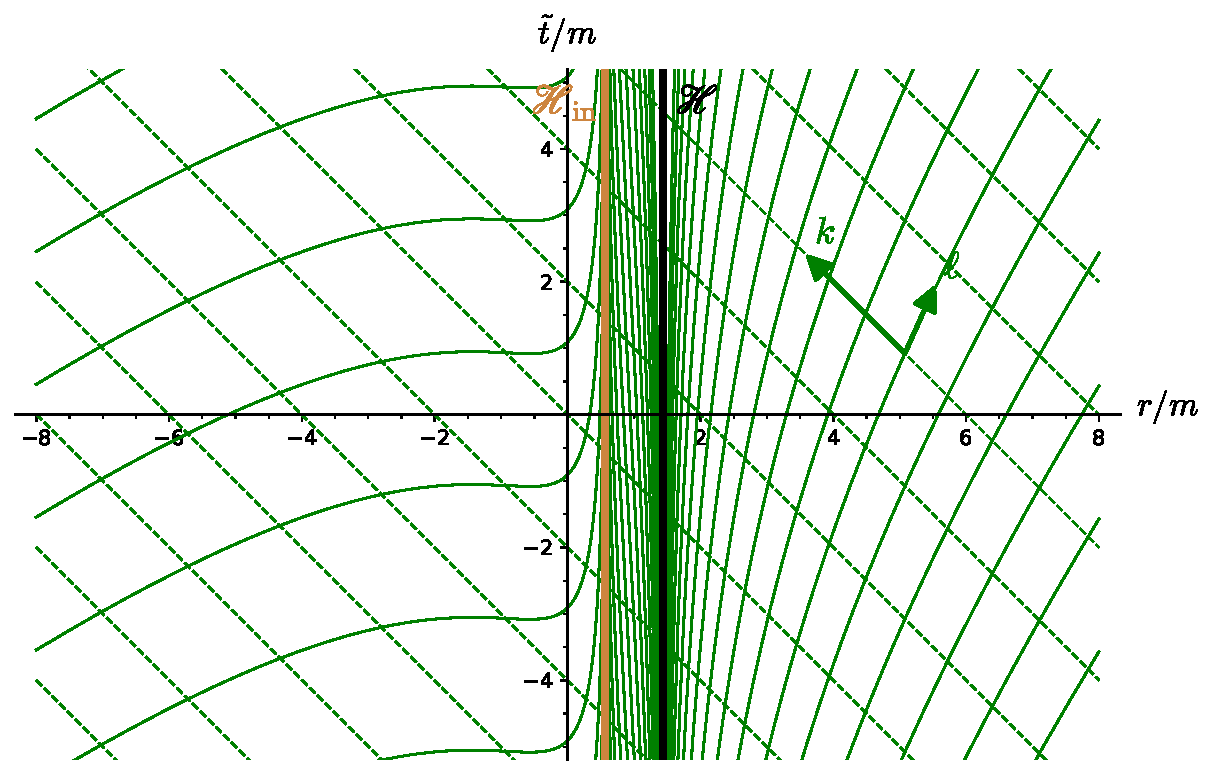
\includegraphics[width=0.9\textwidth]{ker_princ_null_geod_a90.pdf}}
\caption[]{\label{f:ker:princ_null_geod_a90} \footnotesize
Principal null geodesics of Kerr spacetime viewed in terms of the Kerr
coordinates $(\ti,r)$ for $a/m=0.9$. The solid (resp. dashed) curves
correspond to outgoing geodesics $\Li^{\rm out}_{(u,\th,\tilde{\tph})}$
(resp. ingoing geodesics $\Li^{\rm in}_{(v,\th,\tph)}$), as given by
Eq.~(\ref{e:ker:out_princ_geod}) with $u=\mathrm{const}$
(resp. Eq.~(\ref{e:ker:def_t_tilde}) with $v=\mathrm{const}$). The increment
in $u$ between two depicted outgoing geodesics is $\delta u = 2m$;
similarly, two depicted ingoing geodesics differ in their values of
$v$ by $\delta v = 2m$. Note that the outgoing principal null geodesics
tend to become tangent to the horizon $\Hor$ (resp. $\Hor_{\rm in}$) when
$r\to r_+$ (resp. $r\to r_-$). Actually, we shall see in
Sec.~\ref{s:gek:null_gen_hor} and \ref{s:ker:Cauchy_hor}
that the generators of these two horizons belong to the outgoing principal null
congruence.
\textsl{[Figure generated by the notebook \ref{s:sam:Kerr_princ_null_geod}]}
}
\end{figure}

\begin{figure}
\centerline{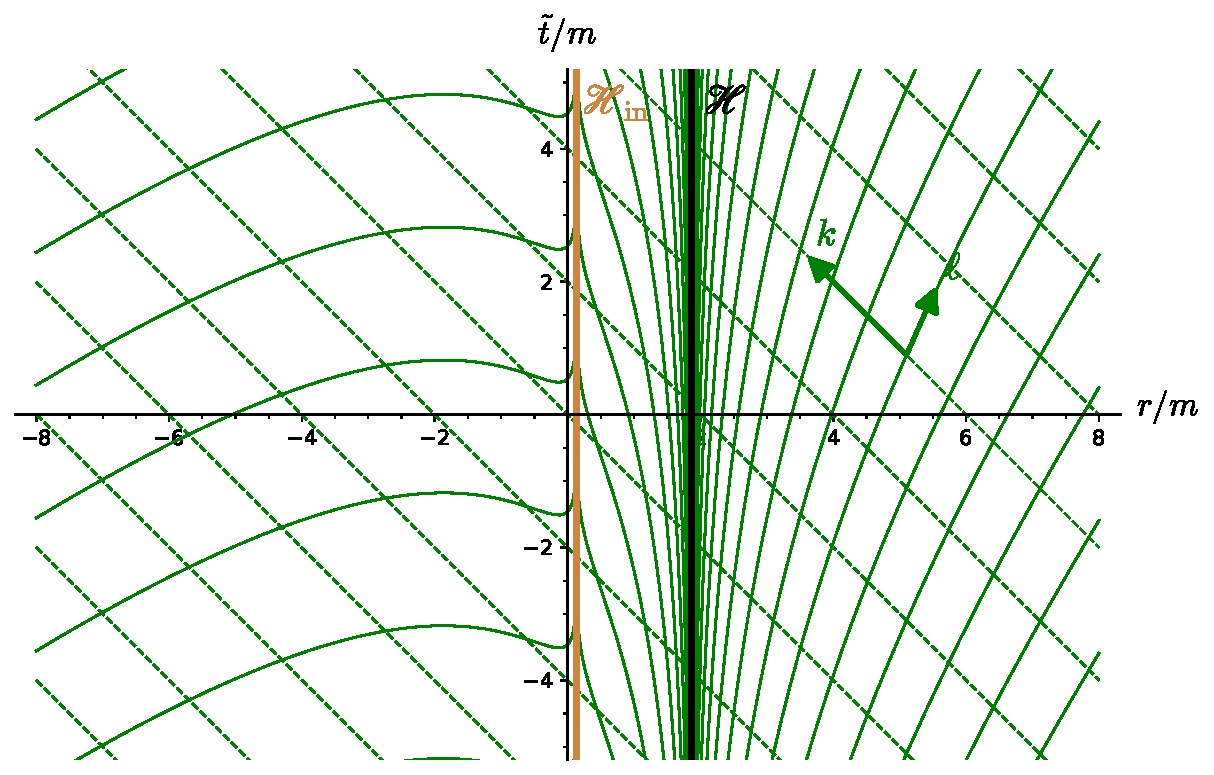
\includegraphics[width=0.9\textwidth]{ker_princ_null_geod_a50.pdf}}
\caption[]{\label{f:ker:princ_null_geod_a50} \footnotesize
Same as Fig.~\ref{f:ker:princ_null_geod_a90}, but for $a/m=0.5$.}
\end{figure}



\subsection{Outgoing principal null geodesics} \label{s:ker:out_princ_null_geod}

One can construct a second congruence of principal null geodesics by considering
the \emph{outgoing} Kerr coordinates instead of the ingoing ones
discussed in Sec.~\ref{s:ker:Kerr_coord}. The
\defin{outgoing null Kerr coordinates}\index{outgoing!null Kerr coordinates}\index{Kerr!coordinates!outgoing null --}
$(u,r,\th,\tilde{\tph})$ are defined by relations to Boyer-Lindquist
coordinates that are similar to
(\ref{e:ker:Kerr_coord}), up to a change of sign:
\begin{subequations}
\label{e:ker:out_Kerr_coord}
\begin{align}
& \dd u = \dd t - \frac{r^2+a^2}{\Delta} \, \dd r \\
& \dd \tilde{\tph} = \dd \ph - \frac{a}{\Delta}\, \dd r .
\end{align}
\end{subequations}
The coordinates $(u,r,\th,\tilde{\tph})$ generalize the null
outgoing Eddington-Finkelstein
coordinates introduced in Sec.~\ref{s:sch:BH} to the case $a\not=0$.
Thanks to the symmetry $(t,\ph)\mapsto(-t,-\ph)$ of the Kerr metric (\ref{e:ker:metric_BL}), which turns $(u,\tilde{\tph})$ into $(-v,-\tph)$, it is clear that the
curves $\Li^{\rm out}_{(u,\th,\tilde{\tph})}$
defined by $(u,\th,\tilde{\tph})=\mathrm{const}$ constitute a second
congruence of principal null geodesics, called the \defin{outgoing principal null geodesics}\index{principal!null geodesic!outgoing --}\index{outgoing!principal null geodesic}.
A priori, this congruence is defined only in $\M_{\rm BL}$, i.e. where $\Delta\neq 0$,
but we shall see below that we can extend it to all $\M$.
As $-r$ was a affine parameter along
the ingoing principal null geodesics, $r$ is an affine parameter along
the outgoing principal null geodesics in $\M_{\rm BL}$.
A difference with respect to the ingoing family is that, while $-r$ was always
increasing towards the future along all ingoing geodesics,
 $r$ is increasing towards the future
along outgoing principal null geodesics only in regions
$\M_{\rm I}$ and $\M_{\rm III}$; in region $\M_{\rm II}$,
$r$ is decreasing towards the future, in agreement with the general
Property~\ref{p:ker:r_decreasing_M_II} (Sec.~\ref{s:ker:time_orientation}).

The fact that the Weyl tensor $\w{C}$
admits two, and exactly two, congruences of principal null geodesics
means that the Kerr metric is an \emph{algebraically special} solution of
the Einstein equation: it belongs to the so-called \emph{Petrov type D}\index{Petrov type}
\cite{ONeil95}.

Let us find
the expression of the outgoing principal null geodesics in terms of
Kerr coordinates (which have been constructed on the
\emph{ingoing} principal null congruence).
Combining (\ref{e:ker:out_Kerr_coord}) with (\ref{e:ker:Kerr_3p1_BL}),
we get
\begin{subequations}
\label{e:ker:out_Kerr_Kerr_3p1}
\begin{align}
& \dd u = \dd \ti - \frac{r^2 + 2m r + a^2}{\Delta} \, \dd r \\
& \dd \tilde{\tph} = \dd \tph - \frac{2a}{\Delta}\, \dd r .
\end{align}
\end{subequations}
These equations can be integrated (cf. the computation leading to Eq.~(\ref{e:ker:Kerr_coord_int})), yielding
\begin{subequations}
\label{e:ker:out_princ_geod}
\begin{align}
& u = \ti - r - \frac{2m}{\sqrt{m^2-a^2}} \left(
    r_+ \ln\left| \frac{r-r_+}{2m} \right|
    - r_- \ln\left| \frac{r-r_-}{2m} \right| \right) \label{e:ker:out_princ_geod_u} \\
&  \tilde{\tph} = \tph - \frac{a}{\sqrt{m^2-a^2}}\, \ln \left|
    \frac{r-r_+}{r-r_-} \right|  ,  \label{e:ker:out_princ_geod_ttph}
\end{align}
\end{subequations}
The quantities $u - \ti$ and $\tilde{\tph} - \tph$ are plotted in terms of
$r$ in Fig.~\ref{f:ker:u_ttphi_r}. We see there that $u$ takes all values
in the range $(-\infty,+\infty)$ in each of the regions $\M_{\rm I}$,
$\M_{\rm II}$ and $\M_{\rm III}$. Accordingly, the 3-tuple
$(u,\th,\tilde{\tph})$ defines uniquely an outgoing principal null geodesic
only in each of these three regions. In other words, the congruence
of outgoing principal null geodesics can be split in
three families
$\Li^{\rm out,I}_{(u,\th,\tilde{\tph})}$,
$\Li^{\rm out,II}_{(u,\th,\tilde{\tph})}$ and
$\Li^{\rm out,III}_{(u,\th,\tilde{\tph})}$,
each family being labelled by $(u,\th,\tilde{\tph})$.
In what follows, we shall denote by $\Li^{\rm out}_{(u,\th,\tilde{\tph})}$ any
member of one of these three families.


\begin{figure}
\centerline{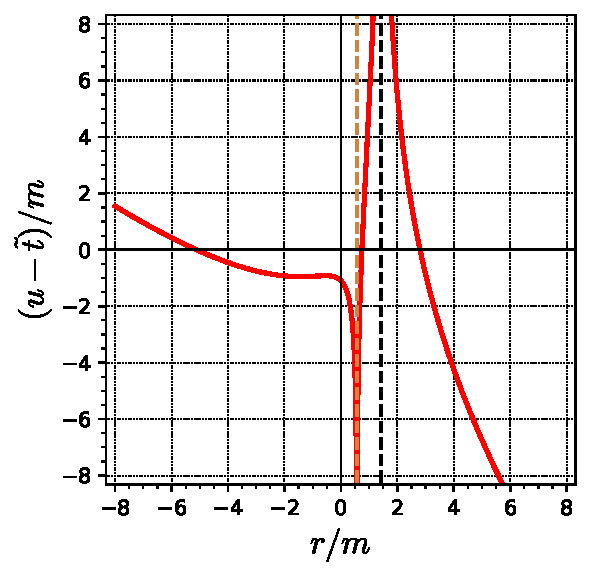
\includegraphics[width=0.4\textwidth]{ker_u_r.pdf}\qquad
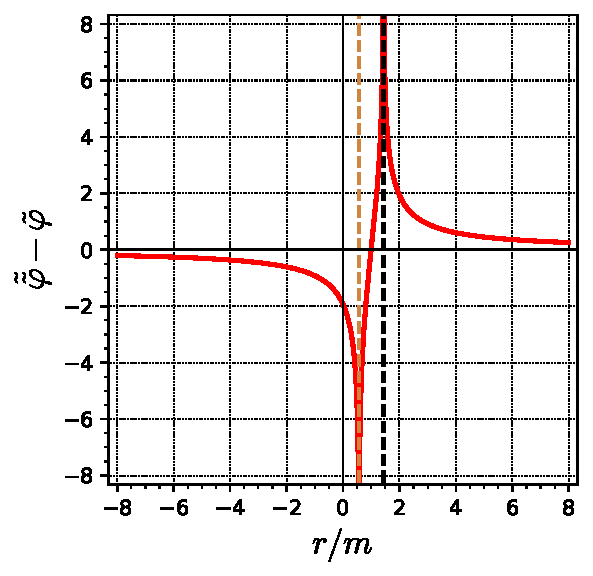
\includegraphics[width=0.4\textwidth]{ker_ttphi_r.pdf}
}
\caption[]{\label{f:ker:u_ttphi_r} \footnotesize
$u - \ti$ (left panel) and $\tilde{\tph} - \tph$ (right panel) as functions
of $r$ given by Eqs.~(\ref{e:ker:out_princ_geod}) for $a/m = 0.9$.
The dashed vertical lines
correspond to $r=r_-$ ($\Hor_{\rm in}$) and $r=r_+$ ($\Hor$) and
delimitate the regions $\M_{\rm III}$, $\M_{\rm II}$ and $\M_{\rm I}$ (from
the left to the right).
\textsl{[Figure generated by the notebook \ref{s:sam:Kerr_princ_null_geod}]}
}
\end{figure}


The outgoing principal null geodesics
are depicted, along with the
ingoing ones, in Figs.~\ref{f:ker:princ_null_geod_a90} and
\ref{f:ker:princ_null_geod_a50}. Note that the $\tph$-motion of the
outgoing geodesics, as expressed by Eq.~(\ref{e:ker:out_princ_geod_ttph}) with $\tilde{\tph}$
held fixed, is not shown in these figures, which represent only traces
in the $(\ti,r)$ plane. Actually the geodesics $\Li^{\rm out}_{(u,\th,\tilde{\tph})}$
are winding with respect the Kerr coordinates $(\ti,r,\th,\tph)$
at the coordinate speed
\be \label{e:ker:wind_speed}
    \left. \frac{\D\tph}{\D\ti} \right| _{\Li^{\rm out}_{(u,\th,\tilde{\tph})}} =
    \frac{2a}{r^2 + 2m r + a^2} .
\ee
\begin{proof}
Along a null geodesic $\Li^{\rm out}_{(u,\th,\tilde{\tph})}$, we have
$\D u = 0$ and $\D\tilde{\tph}=0$, so that (\ref{e:ker:out_Kerr_Kerr_3p1}) yields
\be \label{e:ker:dtdr_dphdr_out}
\left. \frac{\D \ti}{\D r} \right| _{\Li^{\rm out}_{(u,\th,\tilde{\tph})}}  =   \frac{r^2 + 2m r + a^2}{\Delta}  \qquad\mbox{and}\qquad
\left. \frac{\D \tph}{\D r} \right| _{\Li^{\rm out}_{(u,\th,\tilde{\tph})}} = \frac{2a}{\Delta} .
\ee
Dividing the second expression by the first one yields (\ref{e:ker:wind_speed}).
\end{proof}

Note that in both asymptotically flat regions, when $r\rightarrow +\infty$ and
$r\rightarrow -\infty$, the winding speed (\ref{e:ker:wind_speed}) goes to zero
and the two congruences of geodesics tend to $\pm 45^\circ$ lines
in Figs.~\ref{f:ker:princ_null_geod_a90} and
\ref{f:ker:princ_null_geod_a50}, as expected.
Note also that, despite their name, the outgoing principal null geodesics are actually
\emph{ingoing} in $\M_{\rm II}$ (between $\Hor_{\rm in}$ and $\Hor$), i.e. have $r$ decreasing
towards the future, in agreement with Property~\ref{p:ker:r_decreasing_M_II}
(Sec.~\ref{s:ker:time_orientation}).

\begin{remark}
In Fig.~\ref{f:ker:princ_null_geod_a50},
the outgoing geodesics seem to go ``backward in time'' in the region $-2m \lesssim r \lesssim 0$. This
is an artefact due to the hypersurfaces $\ti = \mathrm{const}$ being not spacelike
there, as discussed in Remark~\ref{r:ker:Kerr_slicing}
p.~\pageref{r:ker:Kerr_slicing}.
Consequently it is possible to move to the future with decaying values
of $\ti$ in this region.
The same effect exists, but is less pronounced, for $a/m=0.9$ (Fig.~\ref{f:ker:princ_null_geod_a90}).
\end{remark}

Another view of ingoing principal null geodesics is provided by Figs.~\ref{f:ksm:phi_cut},
\ref{f:ksm:theta_cut} and \ref{f:ksm:2_sheets} of Appendix~\ref{s:ksm}, which
depict them in terms of Kerr-Schild coordinates.

\subsection{Regular null tangent vector to the outgoing congruence}

The presence of $\Delta$ in the denominators of expressions~(\ref{e:ker:dtdr_dphdr_out})
shows that $r$ can no longer be considered as
a parameter along $\Li^{\rm out}_{(u,\th,\tilde{\tph})}$ when
$\Delta=0$, i.e. on $\Hor$ and $\Hor_{\rm in}$. Actually, the family $\Li^{\rm out}_{(u,\th,\tilde{\tph})}$ is not even defined there, since we read on
(\ref{e:ker:out_princ_geod}) and see on Fig.~\ref{f:ker:u_ttphi_r} that
$u\to\pm\infty$ and $\tilde{\tph}\to \pm\infty$ when $r\to r_\pm$ (see also
Fig.~\ref{f:sch:conf_compl2} for a pictorial view of $u\to+\infty$ when $r\to r_+$ in the Schwarzschild limit).
In order to extend the outgoing principal null family to $\Hor$ and $\Hor_{\rm in}$,
let us introduce
along any geodesic $\Li^{\rm out}_{(u,\th,\tilde{\tph})}$ in $\M_{\rm BL}$ the parameter $\lambda$
that is related to the affine parameter $r$ by
\be \label{e:ker:dr_dl_out_princip}
    \frac{\D r}{\D\lambda} = \frac{\Delta}{2(r^2+a^2)} .
\ee
The tangent vector to $\Li^{\rm out}_{(u,\th,\tilde{\tph})}$ associated
to $\lambda$, $\wl$ say, has the following components w.r.t. Kerr coordinates, obtained
by combining Eqs.~(\ref{e:ker:dtdr_dphdr_out}) and (\ref{e:ker:dr_dl_out_princip}):
\begin{align}
& \ell^{\ti} = \frac{\D \ti}{\D\lambda} = \frac{\D \ti}{\D r}\times\frac{\D r}{\D\lambda}
    = \frac{r^2 + 2m r + a^2}{2(r^2+a^2)} = \frac{1}{2} + \frac{m r}{r^2 + a^2} \nonumber \\
& \ell^{r} = \frac{\D r}{\D\lambda} = \frac{\Delta}{2(r^2+a^2)} = \frac{1}{2} - \frac{m r}{r^2 + a^2}\nonumber \\
& \ell^{\th} = \frac{\D \th}{\D\lambda} = 0 \nonumber\\
& \ell^{\tph} = \frac{\D \tph}{\D\lambda} = \frac{\D \tph}{\D r}\times\frac{\D r}{\D\lambda}
    = \frac{a}{r^2+a^2} . \nonumber
\end{align}
In other words, we have
\be \label{e:ker:def_ell_outgoing}
    \encadre{
    \wl = \left( \frac{1}{2} + \frac{m r}{r^2 + a^2} \right) \wpar_\ti
        + \left( \frac{1}{2} - \frac{m r}{r^2 + a^2} \right) \wpar_{\tilde r}
        + \frac{a}{r^2+a^2} \, \wpar_\tph } .
\ee
It is clear that this vector field is regular everywhere in $\M$.
Given the metric components (\ref{e:ker:metric_Kerr_3p1}), it is easy
to check that $\w{g}(\wl,\wl)=0$, i.e. that $\wl$ is a null vector.
Moreover, an explicit computation (cf. the notebook~\ref{s:sam:Kerr_Kerr_coord}) reveals that
\be \label{e:ker:pregeod_ell}
    \wnab_{\wl}\, \wl = \kappa_{\wl} \, \wl,
    \quad\mbox{with}\quad
    \kappa_{\wl} := \frac{m(r^2-a^2)}{(r^2+a^2)^2} .
\ee
Equation~(\ref{e:ker:pregeod_ell}) shows that the integral curves of the
vector field $\wl$ are geodesics (cf. Secs.~\ref{s:def:geod_gener} and \ref{s:geo:gener_param}).
In $\M_{\rm BL}$, they are nothing but the null geodesics $\Li^{\rm out}_{(u,\th,\tilde{\tph})}$.
On $\Hor$ or $\Hor_{\rm in}$, they are null geodesics evolving at constant $r$ ($=r_+$ or $r_-$)
(since $\ell^r = 0$ there),
constant $\th$ (since $\ell^\th = 0$) and constant $\psi$,
where
\be \label{e:ker:psi_tph_ti}
    \psi := \tph - \frac{a}{2 m r_\pm} \ti .
\ee
Indeed, in view of the components (\ref{e:ker:def_ell_outgoing}), we have along these geodesics
\[
    \frac{\D\tph}{\D\ti} = \frac{\D\tph}{\D\lambda} \frac{\D\lambda}{\D\ti}
    = \frac{\ell^\tph}{\ell^\ti} = \frac{2a}{r_\pm^2 + 2 m r_\pm + a^2}
   = \frac{a}{2 m r_\pm}.
\]
Since $a/(2m r_\pm)$ is constant, we get
$\tph = a/(2m r_\pm)\,  \ti + \psi$, where $\psi$ is some integration constant.

\begin{prop}[outgoing principal null geodesics]
Given that $\wl$ is a smooth vector field, the congruence of \defin{outgoing principal null
geodesics}\index{principal!null geodesic!outgoing --}\index{outgoing!principal null geodesic} can be smoothly extended to include the integral curves of $\wl$ on $\Hor$ and
$\Hor_{\rm in}$, which we shall denote by
$\Li^{{\rm out},\Hor}_{(\th,\psi)}$ and $\Li^{{\rm out},\Hor_{\rm in}}_{(\th,\psi)}$,
given that $\th$ and $\psi$ [Eq.~(\ref{e:ker:psi_tph_ti})] are constant
along them. Consequently, the congruence of outgoing principal null
geodesics on $\M$ is made of 5 families:
$\Li^{\rm out,I}_{(u,\th,\tilde{\tph})}$,
$\Li^{\rm out,II}_{(u,\th,\tilde{\tph})}$,
$\Li^{\rm out,III}_{(u,\th,\tilde{\tph})}$,
$\Li^{{\rm out},\Hor}_{(\th,\psi)}$ and $\Li^{{\rm out},\Hor_{\rm in}}_{(\th,\psi)}$,
each family covering a different subset of $\M$.
\end{prop}

\begin{remark}
At the Schwarzschild limit, $a=0$, $\tilde{\tph} = \ph$, $\psi=\ph$ and the
outgoing principal null geodesics
$\Li^{\rm out}_{(u,\th,\tilde{\tph})}$ and
$\Li^{{\rm out},\Hor}_{(\th,\psi)}$ reduce respectively to the
outgoing radial null geodesics
$\Li^{\rm out}_{(u,\th,\ph)}$ and
$\Li^{{\rm out},\Hor}_{(\th,\ph)}$ discussed in Secs.~\ref{s:sch:rad_null_geod} and \ref{s:sch:radial_null_IEF}. This can be seen from the fact that, for $a=0$, the tangent vector
$\wl$ given by Eq.~(\ref{e:ker:def_ell_outgoing}) reduces to the tangent
vector $\wl$ given by Eq.~(\ref{e:sch:null_vector_ell}).
\end{remark}



The 1-form $\uu{\el}$ associated to $\wl$ by
$\w{g}$-duality is obtained
from $\el_{\tilde{\alpha}} = g_{\tilde{\alpha}\tilde{\mu}} \el^{\tilde{\mu}}$, with
$g_{\tilde{\alpha}\tilde{\mu}}$ given by Eq.~(\ref{e:ker:metric_Kerr_3p1}):
\be \label{e:ker:ell_form_Kerr}
    \encadre{ \uu{\el} = - \frac{\Delta}{2(r^2 + a^2)}\, \dd \ti
    + \frac{2\rho^2 - \Delta}{2(r^2 + a^2)}\,  \dd r
    + \frac{a\Delta\sin^2\th}{2(r^2 + a^2)} \, \dd\tph } .
\ee

The components of $\wl$ and $\uu{\el}$ with respect to the Boyer-Lindquist coordinate frame/coframe
are obtained by combining Eq.~(\ref{e:ker:def_ell_outgoing}) with Eq.~(\ref{e:ker:frame_Kerr3p1_BL})
and Eq.~(\ref{e:ker:ell_form_Kerr}) with Eq.~(\ref{e:ker:Kerr_3p1_BL}):
\be \label{e:ker:ell_BL}
    \wl = \frac{1}{2} \wpar_t + \frac{\Delta}{2(r^2 + a^2)}\, \wpar_r
    + \frac{a}{2(r^2 + a^2)}\, \wpar_\ph .
\ee
\be \label{e:ker:ell_form_BL}
    \uu{\el} = - \frac{\Delta}{2(r^2 + a^2)}\, \dd t
     + \frac{\rho^2}{2(r^2 + a^2)}\,  \dd r
     + \frac{a\Delta\sin^2\th}{2(r^2 + a^2)} \, \dd \ph .
\ee


\begin{remark} \label{r:ker:k_versus_l}
The reader may have noticed a certain dissymmetry between the chosen tangent vector
$\w{k}$ of ingoing principal null geodesics, which obeys $\wnab_{\w{k}}\, \w{k} = 0$
[Eq.~(\ref{e:ker:nab_k_k})] and the tangent vector $\wl$ of the outgoing
ones, which obeys $\wnab_{\wl}\, \wl \not= 0$ [Eq.~(\ref{e:ker:pregeod_ell})].
The last property implies that the
parameter $\lambda$ associated to $\wl$ is not affine, while the
parameter $-r$ associated to $\w{k}$ is (cf. Sec.~\ref{s:geo:gener_param}).
The non-affine choice is the price to pay to have a parametrization of the outgoing
congruence well-defined everywhere in $\M$, even where $\Delta=0$. We shall see in
Sec.~\ref{s:ker:max_extension} that in the maximal extension of the Kerr spacetime, there are other regions where these features are reversed,
thereby restoring the symmetry between ingoing and outgoing principal null geodesics
on the extended spacetime.
\end{remark}


Using either the Kerr components (\ref{e:ker:k_ti_tr}) and
(\ref{e:ker:def_ell_outgoing})
or the Boyer-Lindquist components (\ref{e:ker:k_BL}) and (\ref{e:ker:ell_BL}),
one can easily evaluate the scalar product of $\w{k}$ and $\wl$:
\be \label{e:ker:k_scal_ell}
    \w{g}(\w{k},\wl) = - \frac{\rho^2}{r^2 + a^2} .
\ee
This implies that $\w{g}(\w{k},\wl) < 0$ everywhere (note that $\rho^2= 0$
would correspond to the ring singularity $\ring$, which has been excluded from
the spacetime manifold $\M$).
Using Lemma~\ref{p:fra:lem2} (Sec.~\ref{s:fra:time_orientation}) with $\w{u}=\w{k}$ and
$\w{v} = \wl$, we conclude
\begin{prop}[$\wl$ future-directed]
The tangent vector $\wl$ to the outgoing principal null geodesics
is future-directed in all the Kerr spacetime $\M$.
\end{prop}

\begin{remark}
Instead of $\wl$, another natural choice for the tangent vector to the outgoing
principal null geodesics
would have been the tangent vector $\w{\hat{\el}}$
such that $\w{g}(\w{k}, \w{\hat{\el}}) = - 1$.
In view of (\ref{e:ker:k_scal_ell}), the two tangent vectors are related by
$\w{\hat{\el}} = (r^2 + a^2)/\rho^2\,  \wl$
As for $\wl$, the tangent vector $\w{\hat{\el}}$ does not correspond to
an affine parameter of the outgoing
principal null geodesics, i.e. its
non-affinity coefficient $\kappa_{\w{\hat{\el}}}$ is nonzero. While
$\w{\hat{\el}}$ is used in many studies, we prefer $\wl$ here because it
coincides with the Killing vector $\w{\xi} + \Omega_{\Hor} \w{\eta}$
on the event horizon, as we shall see in Sec.~\ref{s:ker:event_hor_gen}
[Eq.~(\ref{e:ker:l_eqH_chi})]. In particular, its
non-affinity coefficient $\kappa_{\w{\el}}$ gives there the so-called
black hole's surface gravity (Sec.~\ref{s:ker:surf_grav} below).
\end{remark}




%%%%%%%%%%%%%%%%%%%%%%%%%%%%%%%%%%%%%%%%%%%%%%%%%%%%%%%%%%%%%%%%%%%%%%%%%%%%%%%

\section{Event horizon} \label{s:ker:event_hor_gen}

\subsection{The two Killing horizons of Kerr spacetime} \label{s:ker:Killing_hor}

Let us consider the hypersurfaces of $\M$ defined by a fixed value of
the coordinate $r$. $\Hor$ and $\Hor_{\rm in}$ are two particular cases,
corresponding to $r=r_+$ and $r=r_-$ respectively.
The normal 1-form to a hypersurface $r=\mathrm{const}$ is $\dd r$; the corresponding
gradient vector field is $\vw{\nabla} r$, the components of which with respect
to Kerr coordinates are
$\nabla^{\tilde{\alpha}} r = g^{\tilde{\alpha}\tilde{\mu}} \partial_{\tilde{\mu}} r
= g^{\tilde{\alpha} r}$, with $g^{\tilde{\alpha} r}$ read on the second raw
of the matrix (\ref{e:ker:inv_met_3p1}). Hence
\[
    \vw{\nabla} r = \frac{2m r}{\rho^2} \wpar_\ti
        +  \frac{\Delta}{\rho^2}\wpar_{\tilde r}
        +  \frac{a}{\rho^2} \wpar_\tph .
\]
Instead of $ \vw{\nabla} r$, it is quite natural to consider the rescaled vector field
\be
    \w{n} := \rho^2 \vw{\nabla} r
\ee
as the normal to the hypersurfaces $r=\mathrm{const}$, for it
has simpler components in the Kerr frame:
\be \label{e:ker:normal_r}
    \w{n} = 2 m r \, \wpar_\ti + \Delta \, \wpar_{\tilde r} + a \, \wpar_\tph .
\ee
The scalar square of $\w{n}$ is
$\w{n}\cdot\w{n} = n_\mu n^\mu = \rho^2 (\nabla_\mu r) n^\mu = \rho^2 n^r$.
Hence, in view of (\ref{e:ker:normal_r}),
\be
    \w{n}\cdot\w{n} = \rho^2 \Delta .
\ee
Since $\rho^2>0$ everywhere on $\M$ and $\Delta = (r-r_+)(r-r_-)$ [Eq.~(\ref{e:ker:def_Delta})], we conclude:
\begin{prop}[causal type of the hypersurfaces $r=\mathrm{const}$]
\begin{itemize}
\item The hypersurfaces $r=\mathrm{const}$ are timelike in regions $\M_{\rm I}$ and $\M_{\rm III}$;
\item The hypersurfaces $r=\mathrm{const}$ are spacelike in region $\M_{\rm II}$;
\item $\Hor$ (where $r=r_+$) and $\Hor_{\rm in}$ (where $r=r_-$) are null hypersurfaces.
\end{itemize}
\end{prop}

On $\Hor$ and $\Hor_{\rm in}$, $\Delta=0$, so that
Eq.~(\ref{e:ker:normal_r})
yields
\be \label{e:ker:normal_r_Killing}
    \w{n} = 2 m r_{\pm} \, \wpar_\ti + a \, \wpar_\tph = 2 m r_{\pm} \, \w{\xi}
        + a \, \w{\eta} ,
\ee
where we have used (\ref{e:ker:Killing_vec_3p1}) and $r_{\pm}$ stands for
$r_+$ on $\Hor$ and $r_-$ on $\Hor_{\rm in}$.
On $\Hor$, we may rewrite this expression as
\be \label{e:ker:n_rp_chi}
    \w{n} = 2 m r_+ \, \w{\chi} ,
\ee
with
\be \label{e:ker:def_chi}
    \encadre{\w{\chi} := \w{\xi} + \Omega_{\Hor} \, \w{\eta} }
\ee
and
\be \label{e:ker:def_OmegaH}
    \encadre{\Omega_{\Hor} := \frac{a}{2 m r_+} = \frac{a}{r_+^2 + a^2}
        = \frac{a}{2m\left( m + \sqrt{m^2-a^2} \right)} }.
\ee
$\Omega_{\Hor}$ being a constant, the vector field $\w{\chi}$ defined by
(\ref{e:ker:def_chi}) is a Killing vector field of $(\M,\w{g})$.
Moreover, Eq.~(\ref{e:ker:n_rp_chi})
shows that this Killing vector is normal to the null hypersurface $\Hor$.
In view of the definition given in Sec.~\ref{s:neh:def_Killing_hor}, we
conclude:
\begin{prop}[$\Hor$ as a Killing horizon]
\label{p:ker:H_Killing}
The hypersurface $\Hor$ defined by $r=r_+$ is a Killing horizon\index{Killing!horizon}\index{horizon!Killing --} with respect to the Killing vector field $\w{\chi}$
[Eq.~(\ref{e:ker:def_chi})].
\end{prop}

Similarly, on $\Hor_{\rm in}$, we may rewrite (\ref{e:ker:normal_r_Killing})
as $\w{n} = 2 m r_- \, \w{\chi}_{\rm in}$, with
\be \label{e:ker:def_chi_in}
    \w{\chi}_{\rm in} := \w{\xi} + \Omega_{\rm in} \, \w{\eta}
\ee
and
\be \label{e:ker:def_Omega_in}
    \Omega_{\rm in} := \frac{a}{2 m r_-} = \frac{a}{r_-^2 + a^2}
        = \frac{a}{2m\left( m - \sqrt{m^2-a^2} \right)} ,
\ee
thereby arriving at:
\begin{prop}[$\Hor_{\rm in}$ as a Killing horizon]
The hypersurface $\Hor_{\rm in}$ defined by $r=r_-$ is a Killing horizon with respect to the Killing vector field $\w{\chi}_{\rm in}$
[Eq.~(\ref{e:ker:def_chi_in})].
\end{prop}
We shall call $\Hor_{\rm in}$ the \defin{inner horizon}\index{inner!horizon}\index{horizon!inner --}. We shall see in Sec.~\ref{s:ker:Cauchy_hor} that $\Hor_{\rm in}$
is actually (part of) a so-called \emph{Cauchy horizon}.

\begin{hist}
The identification of the hypersurfaces $\Hor$ and $\Hor_{\rm in}$
as the only two null hypersurfaces of Kerr spacetime that are stationary
(i.e. Killing horizons in the modern language) has been first performed in
1964 by Robert H. Boyer\index[pers]{Boyer, R.H.}
and T.G. Price\index[pers]{Price, T.G.} \cite{BoyerP65}, who claimed: ``These are `horizons'
in the sense that there can be a flow of matter or radiation across them in only one dimension. They are the analogues of the Schwarzschild null sphere or `singularity'.''
\end{hist}

\subsection{Black hole character} \label{s:ker:event_hor}

As a null hypersurface, $\Hor$ is a one-way membrane (cf. Sec.~\ref{s:def:hor_as_null}),
therefore any (massive or null) particle that crossed it from $\M_{\rm I}$ to
$\M_{\rm II}$ can never be back in $\M_{\rm I}$. Let us show that $\Hor$
is actually a black hole event horizon, as defined in Sec.~\ref{s:glo:def_BH}.

We have seen in Sec.~\ref{s:ker:basic_prop} that the asymptotics of region $\M_{\rm I}$
is the same as that of Schwarzschild spacetime. Hence one can perform a conformal
completion of $(\M_{\rm I},\w{g})$ endowed with a future null infinity $\scri^+$
and a past null infinity $\scri^-$ (an explicit construction of $\scri^+$ and
$\scri^-$ for Schwarzschild spacetime has been performed in
Sec.~\ref{s:max:regul_conf_compl}). A conformal diagram representing $\M_{\rm I}$
along with $\scri^+$
and $\scri^-$ is given in Fig.~\ref{f:ker:3blocks_in} below.


Let us show that the causal past of the future null infinity
coincide with $\M_{\rm I}$: $J^{-}(\scri^+)=\M_{\rm I}$.
Since, as stressed above, no future-directed causal curve can move from $\M_{\rm II}$ to $\M_{\rm I}$
and $\scri^+$ is a boundary of $\M_{\rm I}$, we have $\M_{\rm II} \cap J^{-}(\scri^+) = \varnothing$. A fortiori $\M_{\rm III} \cap J^{-}(\scri^+) = \varnothing$.
We have thus $J^{-}(\scri^+)\subset \M_{\rm I}$. To show the equality between the
two sets there remains to show
that any point $p\in \M_{\rm I}$ can emit a signal reaching $\scri^+$.
Let $\Li$ be the null geodesic through $p$ of the outgoing principal null
congruence $\Li^{\rm out}_{(u,\th,\tilde{\tph})}$ introduced in Sec.~\ref{s:ker:principal_geod}, i.e. $\Li$ is the unique geodesic departing
from $p$ with the tangent vector $\wl$ given by
(\ref{e:ker:def_ell_outgoing}). Along $\Li$, one has
\[
   \frac{\D r}{\D\lambda} = \el^r = \frac{1}{2} - \frac{m r}{r^2 + a^2} ,
\]
where $\lambda$ is the parameter associated with $\wl$.
In particular, at $p$, if we denote by $r_0$ the $r$-coordinate of $p$ in the Kerr system,
\[
    \left. \frac{\D r}{\D\lambda} \right| _{p} = \frac{1}{2} - \frac{m r_0}{r_0^2 + a^2} > 0 .
\]
The above inequality simply translates the fact that $r_0 > r_+$ wherever $p$ lies in
$\M_{\rm I}$.
Hence, initially $r$ is increasing along $\Li$ and we get, since $-mr/(r^2+a^2)$ is an
increasing function of $r$,
\[
    \frac{\D r}{\D\lambda} \geq \frac{1}{2} - \frac{m r_0}{r_0^2 + a^2} =: \alpha > 0.
\]
Since $\alpha$ is a constant, we deduce that
\[
    r \geq r_0 + \alpha(\lambda - \lambda_0) ,
\]
where $\lambda_0$ is the value of $\Li$'s parameter at $p$. When $\lambda\rightarrow +\infty$,
we get $r\rightarrow +\infty$, which proves that the null curve $\Li$
reaches $\scri^+$. Hence we conclude:
\begin{prop}[black hole region in Kerr spacetime]
$\mathscr{B} = \M \setminus \M_{\rm I}$ is the black hole region, the event
horizon of which is $\Hor$.
\end{prop}
Incidentally, since we have already shown that $\Hor$ is a Killing horizon
(Property~\ref{p:ker:H_Killing}),
this illustrates the strong rigidity theorem
(Property~\ref{p:sta:strong_rigidity_thm} in Sec.~\ref{s:sta:strong_rigidity}): the
black hole event horizon of Kerr spacetime
is a Killing horizon.

According to the discussion in Sec.~\ref{s:sta:strong_rigidity}, we may then
call the quantity $\Omega_{\Hor}$ introduced in
Eqs.~(\ref{e:ker:def_chi})-(\ref{e:ker:def_OmegaH}) the
\defin{black hole rotation velocity}\index{black hole!rotation velocity}\index{rotation!velocity}.

\subsection{Null generators of the event horizon} \label{s:gek:null_gen_hor}

The null vector field $\wl$ defined by Eq.~(\ref{e:ker:def_ell_outgoing}) coincides with the Killing vector $\w{\chi}$ on $\Hor$,
since $m r/(r^2 + a^2) \equalH 1/2$ and $a/(r^2+a^2) \equalH \Omega_{\Hor}$:
\be \label{e:ker:l_eqH_chi}
    \wl \equalH \w{\chi} .
\ee
Since (i) $\w{\chi}$ is tangent
to the null geodesic generators of $\Hor$, being a null normal to it (cf. Sec.~\ref{s:def:null_geod_gen}) and (ii) $\wl$ is the tangent vector to the
outgoing principal null geodesics $\Li^{{\rm out},\Hor}_{(\th,\psi)}$ (Sec.~\ref{s:ker:principal_geod}),
we get
\begin{prop}[null generators of the event horizon]
The null generators of the event horizon $\Hor$ are the
geodesics $\Li^{{\rm out},\Hor}_{(\th,\psi)}$
of the outgoing principal null congruence.
\end{prop}

Similarly, we have
\begin{prop}[null generators of the inner horizon]
The null generators of the inner horizon $\Hor_{\rm in}$ are the
geodesics $\Li^{{\rm out},\Hor_{\rm in}}_{(\th,\psi)}$
of the outgoing principal null congruence.
\end{prop}

The reader is referred to Fig.~\ref{f:sta:rot_horizon} for a pictorial
view of the event horizon $\Hor$ spanned by the rotating null generators,
as well as to Figs.~\ref{f:ker:princ_null_geod_a90} and \ref{f:ker:princ_null_geod_a50},
where it appears clearly that at $r=r_+$ (resp. $r=r_-$) the outgoing principal null geodesics are
tangent to $\Hor$ (resp. $\Hor_{\rm in}$).

\begin{remark}
Since $\Delta=0$ on $\Hor$, we read immediately from Eq.~(\ref{e:ker:ell_form_Kerr})
that
\[
    \uu{\el} \equalH \frac{\rho^2}{r^2 + a^2} \, \dd r ,
\]3
which shows that, at any point of $\Hor$, the vector $\wl$ is normal to
the hypersurface $r = \mathrm{const}$ through this point. This hypersurface
being nothing but $\Hor$ itself, we recover the fact that $\wl$ is normal
to $\Hor$.
\end{remark}

In view of expression (\ref{e:ker:def_OmegaH}) for $\Omega_{\Hor}$,
Eq.~(\ref{e:ker:psi_tph_ti}) for the parameter $\psi$
labelling the outgoing principal null geodesics $\Li^{{\rm out},\Hor}_{(\th,\psi)}$
can be rewritten as
\be
    \psi = \tph - \Omega_{\Hor} \ti .
\ee
Hence $\psi$ appears as a corotating azimuthal coordinate on $\Hor$.
Moreover, we verify that the winding speed of the outgoing principal
null geodesics given by Eq.~(\ref{e:ker:wind_speed}) tends toward
$\Omega_{\Hor}$ when approaching the event horizon:
\be
    \lim_{r\rightarrow r_+}
    \left. \frac{\D\tph}{\D\ti} \right| _{\Li^{\rm out}_{(u,\th,\tilde{\tph})}}
    = \Omega_{\Hor} .
\ee
This follows immediately from
$\wl \equalH \w{\chi} = \w{\xi} + \Omega_{\Hor} \w{\eta} = \wpar_{\ti}
    + \Omega_{\Hor} \wpar_{\tph} $
and the identity $r_+^2 + a^2 = 2 m r_+$ (compare Eq.~(\ref{e:ker:wind_speed})
with $r\rightarrow r_+$ and Eq.~(\ref{e:ker:def_OmegaH})).


\subsection{Surface gravity} \label{s:ker:surf_grav}

In view of the pre-geodesic equation (\ref{e:ker:pregeod_ell}) satisfied
by $\wl$ and the identity (\ref{e:ker:l_eqH_chi}), we deduce that
\be \label{e:ker:pregeod_chi}
    \encadre{ \wnab_{\w{\chi}}\, \w{\chi} \equalH \kappa \, \w{\chi} },
\ee
with the non-affinity coefficient\index{non-affinity coefficient} given by Eq.~(\ref{e:ker:pregeod_ell}):
$\kappa = \left. \kappa_{\wl} \right| _{r=r_+} = m(r_+^2-a^2)/(r_+^2+a^2)^2$.
Since $r_+$ is a zero of $\Delta$, we have $r_+^2 + a^2 = 2 m r_+$, so that
$\kappa$ can be rewritten as
\be \label{e:ker:kappa_rp_m_a}
    \kappa = \frac{r_+^2 - a^2}{2r_+(r_+^2+a^2)} = \frac{r_+^2 - a^2}{4m r_+^2} .
\ee
Substituting (\ref{e:ker:def_r_pm}) for $r_+$, we get an expression involving
the two basic Kerr parameters:
\be \label{e:ker:kappa_m_a}
    \encadre{ \kappa = \frac{\sqrt{m^2 - a^2}}{2m(m + \sqrt{m^2-a^2})} } .
\ee
Given the strict inequality $a<m$ assumed in this chapter [Eq.~(\ref{e:ker:a_lower_m})],
we have $\kappa\not=0$. According to the classification introduced in
Sec.~\ref{s:neh:classif_KH}, we may state:
\begin{prop}[non-degeneracy of the event horizon]
As long as $a<m$, the event horizon $\Hor$ is a non-degenerate Killing horizon.
\end{prop}
In Sec.~\ref{s:neh:surface_gravity}, we have seen that the non-affinity coefficient
$\kappa$ can be interpreted as a ``rescaled'' surface gravity. Hence $\kappa$
is called
the \defin{black hole surface gravity}\index{surface!gravity}\index{gravity!surface --}.
The fact that $\kappa$ is a constant (i.e. does not depend on $\th$) is
an illustration of the \emph{zeroth law of black hole mechanics}
established in Sec.~\ref{s:neh:zeroth_law} (cf. in particular
Example~\ref{x:neh:Schw_Kerr_kappa} in that section).
\begin{remark}
As a check, if we let $a\rightarrow 0$ in Eq.~(\ref{e:ker:kappa_m_a}), we get
$\kappa = 1/(4m)$, i.e. we recover the Schwarzschild horizon value computed in
Example~\ref{x:def:Schw_hor3} of Chap.~\ref{s:def} [cf. Eq.~(\ref{e:def:kappa_Schw_hor})].
\end{remark}

\subsection{The Penrose process} \label{s:ker:Penrose_proc}

\begin{figure}
\centerline{\includegraphics[width=0.6\textwidth]{ker_penrose_proc.pdf}}
\caption[]{\label{f:ker:penrose_proc} \footnotesize
Projection in the equatorial plane $t=\mathrm{const}$
and $\th=\pi/2$ of the worldline of a particle and its 4-momentum $\w{p}$,
which decay at event $A$ in two particles: one with 4-momentum
$\w{p'}$, which leaves to infinity, and one with 4-momentum
$\w{p''}$, which falls into the black hole (black region).
The grey zone is the outer ergoregion.
}
\end{figure}

Having established that the black hole event horizon is $\Hor$, i.e.
the boundary between $\M_{\rm I}$ and $\M_{\rm II}$, implies that
one can escape from the outer ergoregion $\mathscr{G}^+$
introduced in Sec.~\ref{s:ker:ergoregion}, since $\mathscr{G}^+ \subset \M_{\rm I}$.
Moreover, we are going to see that $\mathscr{G}^+$  is a region where energy can be extracted ``from''
the black hole. This results from the stationarity Killing
vector $\w{\xi}$ being spacelike there --- the very definition of an
ergoregion. Indeed, let us consider a particle $\mathscr{P}$, of 4-momentum $\w{p}$,
in free fall from infinity into the outer ergoregion. At some point $A\in \mathscr{G}^+$, the particle $\mathscr{P}$
splits (or decays) into two particles: $\mathscr{P}'$, of 4-momentum $\w{p'}$, which leaves to infinity, and $\mathscr{P}''$, of 4-momentum $\w{p''}$, which falls into the black hole (cf. Fig.~\ref{f:ker:penrose_proc}).

We shall define the \emph{energy gain} in the above scenario by
\be \label{e:ker:DE_Penrose_def}
    \Delta E = E_{\rm out} - E_{\rm in} ,
\ee
where $E_{\rm in}$ (resp. $E_{\rm out}$) is the energy of $\mathscr{P}$
(resp. $\mathscr{P}'$) as measured by an inertial observer at rest with respect to the black hole and far from it (cf. Sec.~\ref{s:fra:measure}):
\be \label{e:ker:E_in_out}
    E_{\rm in} = - \left.  \w{\xi} \cdot \w{p} \right| _{\infty}
    \qquad \mbox{and}\qquad
    E_{\rm out} = - \left.  \w{\xi} \cdot \w{p'} \right| _{\infty}  .
\ee
The above formulas hold because the 4-velocity of the inertial observer
is precisely the time-translation Killing vector $\w{\xi} = \wpar_t$
in the far region (since $\w{\xi}\cdot\w{\xi} = g_{tt}  \rightarrow -1$
as  $r\rightarrow +\infty$) (compare with Eq.~(\ref{e:fra:E_obs})).
Assuming that particles $\mathscr{P}$
and $\mathscr{P}'$ are subject only to gravitation, i.e. are in free fall,
their worldlines are timelike geodesics. $\w{\xi}$ being a Killing vector,
it follows then that the scalar products $\w{\xi} \cdot \w{p}$ and
$\w{\xi} \cdot \w{p'}$ are constant along the worldlines of $\mathscr{P}$
and $\mathscr{P}'$ respectively (cf. Sec.~\ref{s:geo:sym}). In particular, we have
$\left. \w{\xi} \cdot \w{p} \right| _{\infty} = \left. \w{\xi} \cdot \w{p} \right| _{A}$
and $\left. \w{\xi} \cdot \w{p'} \right| _{\infty} = \left. \w{\xi} \cdot \w{p'} \right| _{A}$. Accordingly, Eqs.~(\ref{e:ker:DE_Penrose_def}) and
(\ref{e:ker:E_in_out}) leads to
\[
    \Delta E = \left. \w{\xi} \cdot \w{p} \right| _{A} - \left. \w{\xi} \cdot \w{p'} \right| _{A} =
    \left.  \w{\xi} \right| _{A} \cdot (\left. \w{p} \right| _{A}
        - \left. \w{p'} \right| _{A}) .
\]
Now, the conservation of energy-momentum at event $A$
writes $\left. \w{p} \right| _{A} = \left. \w{p'} \right| _{A} + \left. \w{p''} \right| _{A}$, hence
\be \label{e:ker:DE_Penrose}
    \Delta E =   \left. \w{\xi} \cdot \w{p''} \right| _{A} .
\ee
As the 4-momentum of a (non-tachyonic) particle, $\w{p''}$ is always a
future-directed timelike ($\mathscr{P}''$ massive) or null ($\mathscr{P}''$ massless) vector.
If $A$ were located outside the ergoregion, then $\w{\xi}$ would be a
future-directed timelike vector and the scalar product
$ \w{\xi} \cdot  \w{p''}$ would necessarily be negative, leading to
$\Delta E < 0$, i.e. a net loss of energy. However, in the ergoregion,
$\w{\xi}$ is a spacelike vector and it is possible to have $\w{\xi} \cdot \w{p''} > 0$
with $\w{p''}$ future-directed timelike or null.
If this occurs, then $\Delta E > 0$: the outgoing particle has more energy
than the ingoing one. The above process is then called a
\defin{Penrose process}\index{Penrose!process}.
It is particulary relevant to astrophysics, notably via the so-called
\emph{Blanford-Znajek mechanism}\index{Blanford-Znajek mechanism} or via
some magnetohydrodynamical processes (see Ref.~\cite{LasotGATN14} for an extended
discussion).

\begin{remark}
Assuming that the particle $\mathscr{P}''$ follows a geodesic,
the scalar product $\w{\xi} \cdot \w{p''}$ in the right-hand side of Eq.~(\ref{e:ker:DE_Penrose}) is actually constant along the worldline of
$\mathscr{P}''$, so that the mention of the point $A$ can be omitted in
Eq.~(\ref{e:ker:DE_Penrose}).
\end{remark}

\begin{remark} \label{r:ker:negative_energy}
If the Penrose process does occur, i.e. if
$\Delta E > 0$, the particle $\mathscr{P}''$ is called a
\defin{negative-energy particle}\index{negative-energy particle}\index{particle!negative-energy --}. This
stems from the fact that the quantity
$E_\mathscr{P}'' := - \w{\xi}\cdot\w{p''}$ obeys
then $E_\mathscr{P}'' < 0$. However, it should be stressed that
$E_\mathscr{P}''$ does not correspond to a locally measured energy by some
physical observer, as given by formula~(\ref{e:fra:E_obs}), since $\w{\xi}$ cannot be identified with any observer
4-velocity, being spacelike in the ergoregion, where $\mathscr{P}''$ lives.
\end{remark}

\begin{hist}
The Penrose process has first been suggested by Roger Penrose\index[pers]{Penrose, R.}
in 1969,
in the review article \cite{Penro69} (cf. the footnote 7 in this article);
the detailed calculation has been presented subsequently in an
article written with Roger Floyd\index[pers]{Floyd, R.M.} \cite{PenroF71}.
\end{hist}


%%%%%%%%%%%%%%%%%%%%%%%%%%%%%%%%%%%%%%%%%%%%%%%%%%%%%%%%%%%%%%%%%%%%%%%%%%%%%%%

\section{Global quantities} \label{s:ker:global_quantities}

\subsection{Mass} \label{s:ker:Komar_mass}

We have seen in Sec.~\ref{s:ker:basic_prop} that when
$r\rightarrow +\infty$, the Kerr metric tends towards the Schwarzschild
metric of parameter $m$ (cf. Eq.~(\ref{e:ker:asympt_metric}));
we conclude that $m$ is nothing but the gravitational mass $M$ (cf.
Sec.~\ref{s:sch:mass_parameter}).
However, for any asymptotically flat spacetime endowed with
a stationary Killing vector $\w{\xi}$, as the Kerr spacetime,
there is a well-defined concept of mass, namely the \emph{Komar mass}\index{Komar!mass}\index{mass!Komar --}
introduced in Sec.~\ref{s:sta:Komar_mass}.
Let us show explicitly that for the Kerr spacetime, the Komar mass coincides with $m$.
To this aim, we shall use expression~(\ref{e:sta:M_Komar_partial_der}) with $n=4$
for the Komar mass. We shall consider the Boyer-Lindquist coordinates
$(x^\alpha) = (t,r,\th,\ph)$ and define $\Sp$ to be a sphere
$(t,r)=\mathrm{const}$. Coordinates on $\Sp$ are then
$(x^2,x^3)=(\th,\ph)$. Moreover, since the value of $M_\Sp$ does not depend on
the choice of $\Sp$ (cf. Property~\ref{p:sta:Komar_mass_invariant}),
we may set $r\rightarrow +\infty$ and use the
asymptotic flatness of Kerr metric to get simple expressions. The unit normals
to $\Sp$ are then $\w{n} = \wpar_t$ and $\w{s} = \wpar_r$. Moreover, when
$r\rightarrow +\infty$, $\sqrt{q} = r^2\sin\th$. Hence Eq.~(\ref{e:sta:M_Komar_partial_der})
with $n=4$ yields
\[
    M = -\frac{1}{8\pi} \lim_{r\rightarrow +\infty}
        \int_{\Sp}
        (\partial_r \xi_t - \underbrace{\partial_t \xi_r}_{0} )
        r^2\sin\th \, \D\th\, \D\ph ,
\]
with
\[
    \xi_t = g_{t\mu} \xi^\mu = g_{t\mu} \delta^\mu_{\ \, t}
        = g_{tt} \simeq - 1 + \frac{2m}{r} ,
\]
the last expression resulting from the expansion (\ref{e:ker:asympt_metric}).
We have then $\partial_r \xi_t = -2m/r^2$, so that the above integral yields
\be \label{e:ker:M_m}
    \encadre{M = m} .
\ee


\subsection{Angular momentum} \label{s:ker:Komar_J}

Since the Kerr spacetime is axisymmetric, a well-defined notion
of angular momentum is provided by the
\emph{Komar angular momentum}\index{Komar!angular momentum}\index{angular!momentum!Komar --}
$J$ introduced in Sec.~\ref{s:sta:Komar_angu_mom}.
Let us compute $J$ via Eq.~(\ref{e:sta:J_Komar_partial_der}) by means of
Boyer-Lindquist coordinates, choosing
for $\Sp$ a 2-sphere $(t,r)=\mathrm{const}$.
In evaluating the terms $s^\mu \partial_\mu \eta_\nu \, n^\nu$
and $n^\mu \partial_\mu \eta_\nu \, s^\nu$ as $r\rightarrow+\infty$, we have
to be a little more cautious than in Sec.~\ref{s:ker:Komar_mass}, since
one of
the components $\eta_\alpha$ is diverging when $r\rightarrow+\infty$:
\[
    \eta_\alpha = g_{\alpha\mu} \, \eta^\mu = g_{\alpha\mu} \, \delta^\mu_{\ \, \ph}
        = g_{\alpha\ph} = (g_{t\ph},0,0,g_{\ph\ph})
\]
with, according to (\ref{e:ker:asympt_metric}),
$g_{\ph\ph} \sim r^2\sin^2\th$ as $r\rightarrow+\infty$.
Moreover, given the value of $g_{t\ph}$ read on (\ref{e:ker:metric_BL}), we may
write
\[
    \eta_\alpha \sim \left( - \frac{2 a m \sin^2\th}{r}, 0, 0, r^2\sin^2\th \right)
        \quad\mbox{when}\quad
        r\rightarrow+\infty .
\]
Let us choose for the timelike normal $\w{n}$ to $\Sp$
the future-directed unit normal to the hypersurfaces $t=\mathrm{const}$:
\be \label{e:ker:un_Ndt}
 \uu{n} = - N \dd t,
\ee
where $N$ is a normalization factor ensuring $\w{n}\cdot\w{n}=-1$.
We do not need the precise value\footnote{It is given by Eq.~(\ref{e:ker:lapse_ZAMO}) below.} of $N$, but simply the property $N\rightarrow 1$
as $r\rightarrow+\infty$.
We have then
$n_\alpha = (-N,0,0,0)$, so that
\[
    n^\alpha = g^{\alpha\mu} n_\mu = g^{\alpha t} (-N) =
    (- N g^{tt}, 0, 0, - N g^{t\ph} ),
\]
where the last equality follows from the
expression (\ref{e:ker:inv_met_BL}) of $g^{\alpha\beta}$ in
Boyer-Lindquist coordinates, with $g^{tt} \sim -1$ and
$g^{t\ph} \sim - 2 a m / r^3$ when $r\rightarrow+\infty$; hence
\[
    n^\alpha \sim \left( 1, 0, 0, \frac{2 a m}{r^3} \right)  \quad\mbox{when}\quad
        r\rightarrow+\infty .
\]
The choice of $\w{n}$ completely determines that of $\w{s}$:
\[
    s^\alpha = \left( 0, \frac{\sqrt{\Delta}}{\rho}, 0, 0 \right)
        \sim (0,1,0,0) \quad\mbox{when}\quad r\rightarrow+\infty .
\]
Indeed, given the metric components (\ref{e:ker:metric_BL}), we immediately
check that $\w{n}\cdot\w{s}=0$, $\w{s}\cdot\w{s}=1$ and
$\uu{s} = (\rho/\sqrt{\Delta})\, \dd r$, which does imply that $\w{s}$ is normal to $\Sp$.

Given the above expressions for $\eta_\alpha$, $n^\alpha$ and $s^\alpha$,
we get, for $r\rightarrow+\infty$,
\[
  s^\mu \partial_\mu \eta_\nu \, n^\nu \sim \partial_r \left( - \frac{2 a m \sin^2\th}{r} \right) \times 1 + \partial_r \left(r^2 \sin^2\th \right) \times \frac{2 a m}{r^3}
    \sim \frac{6 a m \sin^2\th}{r^2}
\]
and
\[
    n^\mu \partial_\mu \eta_\nu \, s^\nu \sim \partial_t \underbrace{\eta_r}_{0}
        + \frac{2 a m}{r^3} \partial_\ph \underbrace{\eta_r}_{0}  = 0 .
\]
Hence Eq.~(\ref{e:sta:J_Komar_partial_der}) leads to
\[
    J = \frac{1}{16\pi} \lim_{r\rightarrow +\infty}
        \int_{\Sp}
        \frac{6 a m \sin^2\th}{r^2} \times
        r^2\sin\th \, \D\th\, \D\ph  =
        \frac{3 a m}{8\pi} \int_{\Sp} \sin^3\th \, \D\th\, \D\ph
        = \frac{3 a m}{4} \underbrace{\int_0^\pi \sin^3\th \, \D\th}_{4/3} ,
\]
i.e.
\be \label{e:ker:J_am}
    \encadre{J = a m } .
\ee
We conclude that the parameter $a$ is nothing but the total angular momentum
divided by the total mass.

\subsection{Black hole area}

Since the event horizon $\Hor$ is a Killing horizon (cf. Sec.~\ref{s:ker:Killing_hor}),
it is a non-expanding horizon. As such, it has a well-defined
area\index{area!of the Kerr black hole} $A$, which is the
common area of any of its cross-sections, as we have seen in
Sec.~\ref{s:neh:invar_area}. To compute $A$, we shall not use Boyer-Lindquist
coordinates as for $M$ and $J$, because they are singular on $\Hor$; we shall
use rather the Kerr coordinates $(\ti, r, \th,\tph)$, which are regular
on $\Hor$. $\Hor$ is defined by $r=r_+$ and it is natural to consider a
cross-section of it, $\Sp$ say, defined by $\{\ti=\mathrm{const}, r=r_+\}$.
Then $\Sp$ is spanned by the coordinates $(x^a) = (\th,\tph)$ and the metric $\w{q}$
induced on it by the spacetime metric is obtained by setting $r=r_+$,
$\dd\ti=0$ and $\dd r = 0$ in (\ref{e:ker:metric_Kerr_3p1}):
\[
        \w{q} =
   (r_+^2 + a^2\cos^2\th)\, \dd \th^2
    + \left( r_+^2 + a^2 + \frac{2 a^2 m r_+ \sin^2\th}{r_+^2 + a^2\cos^2\th} \right)
    \sin^2\th \, \dd \tph^2 .
\]
Now, since $r_+$ is a zero of $\Delta$ [cf. Eq.~(\ref{e:ker:def_Delta})],
we have $2 m r_+ = r_+^2 + a^2 $. This brings us to
\be \label{e:ker:q_cross_section_H}
        \w{q} =
  (r_+^2 + a^2\cos^2\th) \, \dd \th^2
    + \frac{(r_+^2 + a^2)^2}{r_+^2 + a^2\cos^2\th}\,
    \sin^2\th \, \dd \tph^2 .
\ee
The area of the cross-section $\Sp$ is
\[
    A = \int_\Sp \sqrt{q} \, \D\th\, \D\tph
      = (r_+^2 + a^2) \underbrace{\int_\Sp \sin\th \, \D\th\, \D\tph}_{4\pi}
\]
where we have used (\ref{e:ker:q_cross_section_H}) to write
$q = \det (q_{ab}) = (r_+^2 + a^2)^2 \sin^2\th$.
We have thus
\be \label{e:ker:A_rp_a_m}
    \encadre{A = 4\pi (r_+^2 + a^2) = 8 \pi m r_+} .
\ee
Via (\ref{e:ker:def_r_pm}),
one may recast this result to let appear only $m$ and $a$:
\be \label{e:ker:A_a_m}
    \encadre{A = 8 \pi m (m + \sqrt{m^2-a^2})} .
\ee

\subsection{Smarr formula}

By combining the relations $\Omega_{\Hor} = a/(2 m r_+)$ [Eq.~(\ref{e:ker:def_OmegaH})],
$\kappa = (r_+^2 - a^2)/(4 m r_+^2)$ [Eq.~(\ref{e:ker:kappa_rp_m_a})]
and $A = 8\pi m r_+$ [Eq.~(\ref{e:ker:A_rp_a_m})], we get an interesting
identity:
\[
    \frac{\kappa A}{4\pi} + 2 \Omega_{\Hor} a m   = m .
\]
If we let appear the total angular momentum $J = a m$ [Eq.~(\ref{e:ker:J_am})]
and the Komar mass $M = m$ [Eq.~(\ref{e:ker:M_m})], we can turn this identity
into
\be \label{e:ker:Smarr}
    \encadre{ M =  \frac{\kappa A}{4\pi} + 2 \Omega_{\Hor} J} .
\ee
This is actually the particular case $\w{T} = 0$ (vacuum) of the generic
\emph{Smarr formula}\index{Smarr formula} (\ref{e:sta:Smarr_M_infty_n4})
established in Chap.~5, or the particular
case $Q_{\Hor}=0$ (vanishing electric charge) of the electrovacuum Smarr formula
(\ref{e:sta:Smarr_electrovac_n4}).

%%%%%%%%%%%%%%%%%%%%%%%%%%%%%%%%%%%%%%%%%%%%%%%%%%%%%%%%%%%%%%%%%%%%%%%%%%%%%%%

\section{Families of observers in Kerr spacetime} \label{s:ker:observers}

The concept of \emph{observer} in a relativistic spacetime
has been recalled in Sec.~\ref{s:fra:measure}.
We discuss here some families of observers well adapted to Kerr spacetime:
the ZAMOs (Sec.~\ref{s:ker:ZAMO}) and the Carter observers (Sec.~\ref{s:ker:Carter_obs}).
These two families are actually particular cases of a more general concept, that
of a \emph{stationary observer}, which we introduce first.

\subsection{Stationary observers} \label{s:ker:station_obs}

A \defin{stationary observer}\index{stationary!observer!in Kerr spacetime}\index{observer!stationary --}
is an observer $\Obs$ in Kerr spacetime whose 4-velocity $\w{u}$ is a linear
combination of the Killing vectors $\w{\xi}$ and $\w{\eta}$ with constant coefficients\footnote{In
the definition (\ref{e:ker:4vel_stationary_obs}), the coefficients $\alpha$ and $\beta$
are required to be constant along a given observer's worldline. When considering a family of observers,
they may vary from one worldline to the other.}:
\be \label{e:ker:4vel_stationary_obs}
    \w{u} = \alpha \, \w{\xi} + \beta \, \w{\eta} , \qquad \alpha=\mathrm{const},\ \beta=\mathrm{const} .
\ee
It follows that the worldline $\Li$ of $\Obs$ is an
orbit of the isometry group $\R\times\mathrm{SO}(2)$ of Kerr spacetime. In physical terms,
this means that the spacetime geometry as perceived by observer $\Obs$ does not evolve,
hence the name \emph{stationary observer}.

A stationary observer moves necessarily at fixed values of the non-ignorable coordinates
in a coordinate system adapted to the spacetime symmetries, like Boyer-Lindquist coordinates or Kerr
ones. For instance, considering the Boyer-Lindquist coordinates $(t, r, \th, \ph)$,
we have $\w{\xi} = \wpar_t$ and $\w{\eta} = \wpar_\ph$ and
we deduce from (\ref{e:ker:4vel_stationary_obs}) and the definition (\ref{e:fra:def_u}) of the
4-velocity that along the worldline $\Li$:
\[
    \frac{\D t}{\D\tau} = \alpha,\quad
    \frac{\D r}{\D\tau} = 0,\quad
    \frac{\D \th}{\D\tau} = 0,\quad
    \frac{\D \ph}{\D\tau} = \beta,
\]
where $\tau$ is the observer's proper time. It follows that
the stationary observer evolves at fixed values of the coordinates $r$ and $\th$.

Outside the Carter time machine $\mathscr{T}$ (cf. Sec.~\ref{s:ker:time_machine}), we have
necessarily $\alpha\neq 0$, because $\w{\eta}$ is spacelike in $\M\setminus\mathscr{T}$
and the 4-velocity $\w{u}$ is necessarily timelike. Hence,
by introducing $\omega := \beta/\alpha$, we may rewrite
(\ref{e:ker:4vel_stationary_obs}) as
\be \label{e:ker:4vel_stat_obs_omega}
    \encadre{ \w{u} = \alpha \left( \w{\xi} + \omega \, \w{\eta} \right)}, \qquad \alpha=\mathrm{const},\ \omega=\mathrm{const} .
\ee
The coefficient $\omega$ gives the rate of variation of the azimuthal coordinate along the observer's worldline $\Li$
in any coordinate system adapted to the spacetime symmetries, like the Boyer-Lindquist ones
$(t,r,\th,\ph)$, the Kerr ones $(\ti, r, \th, \tph)$, or the null Kerr ones $(v,r,\th,\tph)$,
according to
\be \label{e:ker:omega_angular_vel}
    \encadre{ \omega = \left. \frac{\D\ph}{\D t} \right| _\Li  =
    \left. \frac{\D\tph}{\D v} \right| _\Li = \left. \frac{\D\tph}{\D \ti} \right| _\Li } .
\ee
\begin{proof}
Let us consider Boyer-Lindquist coordinates $(t,r,\th,\ph)$. Denoting by $\tau$
the proper time of $\Obs$, we have
$\D\ph/\D t |_\Li= {\D \ph}/{\D \tau} \times {\D \tau}/{\D t}$. Now by the
definition (\ref{e:fra:def_u}) of the 4-velocity, ${\D \ph}/{\D \tau} = u^\ph$
and ${\D \tau}/{\D t} = (u^t)^{-1}$. We have thus $\D\ph/\D t |_\Li= u^\ph/u^t$.
From Eq.~(\ref{e:ker:4vel_stat_obs_omega}) along with
$\w{\xi} = \wpar_t$ and $\w{\eta} = \wpar_\ph$, we read $u^t = \alpha$
and $u^\ph = \alpha\omega$. Hence $\D\ph/\D t |_\Li=\omega$.
The same demonstration applies to Kerr and null Kerr coordinates because
$\w{\xi} = \wpar_v = \wpar_{\ti}$ and $\w{\eta} = \wpar_{\tph}$.
\end{proof}
\begin{remark}
That the ratios $\D\ph/\D t$, $\D\tph/\D v$ and $\D\tph/\D \ti$ along $\Li$
are all equal, as expressed in (\ref{e:ker:omega_angular_vel}), is not
surprising if one considers the links between the various coordinates
expressed by Eqs.~(\ref{e:ker:Kerr_coord_v}), (\ref{e:ker:Kerr_coord_tph}) and (\ref{e:ker:Kerr_3p1_BL}).
Setting $\D r = 0$ in these equations, since $r$ is constant along $\Li$, we get
\[
    \D t |_\Li = \D v |_\Li = \D\ti |_\Li \qand
    \D \ph |_\Li = \D \tph | _\Li .
\]
\end{remark}

Equation~(\ref{e:ker:omega_angular_vel}) allows for a nice physical interpretation of
$\omega$. Indeed, we have seen in Sec.~\ref{s:ges:circular_orbits} [cf. Eq.~(\ref{e:ges:def_Omega})]
that $\D\ph/\D t |_\Li$ is nothing
but the angular velocity around the symmetry axis as measured by an asymptotically distant inertial observer.
The demonstration was performed in the Schwarzschild case and for a circular orbit in the equatorial plane, but
it used only the stationarity of Schwarzschild spacetime and the fact that ${\D\ph}/{\D t}$ was constant
along $\Li$, so it applies to the present case as well.


\subsection{Static observers} \label{s:ker:static_obs}

A \defin{static observer}\index{static!observer!in Kerr spacetime}\index{observer!static --}
is a stationary observer $\Obs$ having $\omega = 0$.
The denomination stems from the fact that the three coordinates $(r,\th,\ph)$
(or $(r,\th,\tph)$)
remain constant along $\Obs$'s worldline, since $\omega = 0$ in Eq.~(\ref{e:ker:omega_angular_vel})
implies $\ph = \mathrm{const}$ and $\tph = \mathrm{const}$. Moreover, such an
observer appears not moving to an asymptotic inertial observer.

According to (\ref{e:ker:4vel_stat_obs_omega}) with $\omega=0$, the 4-velocity of $\Obs$ is collinear to the Killing vector $\w{\xi}$: $\w{u} = \alpha \w{\xi}$. We conclude that a static
observer can exist only where $\w{\xi}$ is timelike, i.e. outside the ergoregion (cf. Sec.~\ref{s:ker:ergoregion}). This explains why the outer boundary of the ergoregion
(the ergosphere) is sometimes called the \emph{static limit}\index{static!limit} (cf. Remark~\ref{r:ker:static_limit} on p.~\pageref{r:ker:static_limit}).

Since static observers are not very useful for describing physical processes
in the vicinity of a Kerr black hole (in particular, they cannot exist
close to the event horizon, which is located in the ergoregion), we shall not
discuss them further.


\subsection{Zero-angular-momentum observers (ZAMO)} \label{s:ker:ZAMO}

Let us consider an observer $\Obs$ whose worldline is normal to the hypersurfaces
of constant Boyer-Lindquist coordinate $t$, $\Sigma_t$ say. Of course, such an observer exists
only where the hypersurface $\Sigma_t$ is spacelike, so that the latter has
a timelike normal (cf. Sec.~\ref{s:def:hor_as_null}). A normal 1-form to $\Sigma_t$ is
of course $\dd t$. The associated normal vector, $\w{N}$ say, is obtained
by metric duality [cf. Eq.~(\ref{e:bas:arrow_form})-(\ref{e:bas:arrow_form_comp})]:
\be \label{e:ker:N_grad_t}
    \w{N} = - \overrightarrow{\dd t} = -\vw{\nabla} t .
\ee
In components:
\[
   N^\alpha = - g^{\alpha\mu} (\D t)_\mu = - g^{\alpha\mu} \delta^t_{\ \, \mu} = - g^{t\alpha} .
\]
The minus sign has been chosen to have $\w{N}$ future-directed, as we shall see below.
In view of the Boyer-Lindquist components (\ref{e:ker:inv_met_BL}) of the inverse metric,
we get
\be \label{e:ker:normal_ZAMO}
    \w{N} = \frac{1}{\Delta}
    \left( r^2 + a^2 + \frac{2 a^2 m r \sin^2\th}{\rho^2} \right) \, \wpar_t
     + \frac{2 a m r}{\rho^2 \Delta} \, \wpar_\ph .
\ee
The scalar square of $\w{N}$ is
\be \label{e:ker:w_square}
    \w{N}\cdot\w{N} = \w{g}(\w{N},\w{N}) = N_\mu N^\mu = \delta^t_{\ \, \mu} N^\mu = N^t
    = - \frac{1}{\Delta}
    \left( r^2 + a^2 + \frac{2 a^2 m r \sin^2\th}{\rho^2} \right) .
\ee
Now, the quantity inside the parentheses is positive everywhere except in
the Carter time machine\index{Carter!time machine}\index{time!machine (Carter)} $\mathscr{T}\subset \M_{\rm III}$ discussed in Sec.~\ref{s:ker:time_machine}.
Indeed, up to the factor $\sin^2\th \geq 0$, it coincides with
expression~(\ref{e:ker:eta_square}) of $\w{\eta}\cdot\w{\eta}$.
Since $\Delta = (r - r_+)(r - r_-)$ is positive on
$\M_{\rm I}$ and $\M_{\rm III}$, and negative on $\M_{\rm II}$, we conclude that
the locus where $\w{N}$ is timelike is
\be \label{e:ker:ZAMO_domain}
    \M_{\rm ZAMO} := \M_{\rm I} \cup (\M_{\rm III}\setminus \mathscr{T}) .
\ee
This is thus the region where the observer $\Obs$ is defined.
Note that it does not contain the horizons $\Hor$ and $\Hor_{\rm in}$, which
is not surprising since Boyer-Lindquist coordinates are singular there,
notably in terms of the spacetime slicing by the hypersurfaces $\Sigma_t$,
as illustrated in Fig.~\ref{f:sch:SD_slices} for the case $a=0$.

In all $\M_{\rm ZAMO}$,
the timelike vector $\w{N}$ is future-directed with respect to the time orientation chosen in
Sec.~\ref{s:ker:time_orientation}.
Indeed, the latter is set by the global null
vector field $\w{k}$ and we have, using the Boyer-Lindquist components
(\ref{e:ker:k_BL}) of $\w{k}$:
\[
    \w{k}\cdot\w{N} = N_\mu k^\mu = - k^t = - \frac{r^2 + a^2}{\Delta} < 0
    \ \mbox{on} \ \M_{\rm ZAMO} ,
\]
so that Lemma~\ref{p:fra:lem2} [cf. Eq.~(\ref{e:fra:orient_null1})]
let us conclude that
$\w{N}$ is future-directed.

Choosing the observer $\Obs$ as having his worldline orthogonal to $\Sigma_t$
means that $\Obs$'s 4-velocity $\w{n}$ is the unit timelike vector introduced
by Eq~(\ref{e:ker:un_Ndt}). Equivalently, $\w{n}$ is $\w{N}$ rescaled to form a unit vector:
\be \label{e:ker:def_n_ZAMO}
    \w{n} = N \w{N} = - N \vw{\nabla} t ,
\ee
with\footnote{Note that $N$ is not defined as the (pseudo)norm of $\w{N}$, as the notation might suggest, but rather as the inverse of it.} $N := (-\w{N}\cdot\w{N})^{-1/2}$.
In view of Eq.~(\ref{e:ker:w_square}), we get
\be \label{e:ker:lapse_ZAMO}
    N = \sqrt{\Delta} \left( r^2 + a^2 + \frac{2 a^2 m r \sin^2\th}{\rho^2} \right) ^{-1/2} .
\ee
$N$ is called the \defin{lapse function}\index{lapse function}, for it relates the increment $\D\tau$
in the proper time of $\Obs$ to the change $\D t$ of the coordinate $t$ when moving from $\Sigma_{t}$ to $\Sigma_{t + \D t}$ via
\be \label{e:ker:dtau_lapse}
    \encadre{ \D\tau = N \D t }.
\ee
\begin{proof}
The infinitesimal vector that connects the point of proper time $\tau$ to that of proper time $\tau+\D\tau$ along $\Obs$'s worldline is $\D \w{x} = \D\tau\,  \w{n}$ (by the very definition of the 4-velocity $\w{n}$, compare Eq.~(\ref{e:fra:def_u})). The corresponding increment in the coordinate $t$ is given by
formula (\ref{e:bas:df}): $\D t = \langle \dd t, \D \w{x} \rangle$; we have then, using Eq.~(\ref{e:ker:def_n_ZAMO}) to express $\vw{\nabla} t$,
\[
    \D t = \langle \dd t, \D \w{x} \rangle = \vw{\nabla} t \cdot \D \w{x} = \D\tau \, \vw{\nabla} t \cdot \w{n}
    = - \frac{\D\tau}{N} \underbrace{\w{n}\cdot\w{n}}_{-1} = \frac{\D\tau}{N} ,
\]
hence formula (\ref{e:ker:dtau_lapse}).
\end{proof}

A \defin{zero-angular-momentum observer (ZAMO)}\index{zero-angular-momentum observer}\index{ZAMO}
is an observer $\Obs$ of the above type, i.e. whose worldline $\Li$ is normal to the
hypersurfaces $\Sigma_t$ of constant Boyer-Lindquist time $t$, and whose orthonormal frame\index{ZAMO!frame}\index{frame!ZAMO --}
$(\w{e}_{(\alpha)})$ is related to the Boyer-Lindquist coordinate frame $(\wpar_\alpha)$ by
\begin{subequations}
\label{e:ker:def_ZAMO_frame}
\begin{align}
  & \w{e}_{(0)} = \w{n} =
  \frac{\sqrt{\rho^2(r^2 + a^2) + 2 a^2 m r \sin^2\th}}{\rho \sqrt{\Delta}} \,
  \wpar_t + \frac{2 a m r}{\rho \sqrt{\Delta[ \rho^2(r^2 + a^2) + 2 a^2 m r \sin^2\th]}}\, \wpar_\ph
    \label{e:ker:ZAMO_frame_0}\\
  & \w{e}_{(r)} = \frac{\sqrt{\Delta}}{\rho} \, \wpar_r \\
  & \w{e}_{(\th)} = \frac{1}{\rho} \, \wpar_\th \\
  & \w{e}_{(\ph)} =  \frac{\rho}{\sin\th \sqrt{\rho^2(r^2 + a^2) + 2 a^2 m r \sin^2\th}} \,
  \wpar_\ph , \label{e:ker:ZAMO_frame_ph}
\end{align}
\end{subequations}
where $\rho := \sqrt{r^2 + a^2 \cos^2\th}$ (the positive square root of $\rho^2$, which is
defined by Eq.~(\ref{e:ker:def_rho2})).
Expression (\ref{e:ker:ZAMO_frame_0}) for $\w{n}$ has been obtained by
combining Eqs.~(\ref{e:ker:def_n_ZAMO}), (\ref{e:ker:lapse_ZAMO}) and (\ref{e:ker:normal_ZAMO}).
Given the Boyer-Lindquist components (\ref{e:ker:metric_BL}) of $\w{g}$, one readily check
that $(\w{e}_{(r)}, \w{e}_{(\th)},\w{e}_{(\ph)})$ is an orthonormal basis of spacelike vectors
(see the notebook~\ref{s:sam:Kerr_ZAMO_frame} for a SageMath computation).
Moreover, these vectors are all tangent to $\Sigma_t$, since $(\wpar_r, \wpar_\th, \wpar_\ph)$ are.
They are thus orthogonal to $\w{n}=\w{e}_{(0)}$, which is a unit timelike vector. This completes the proof that
$(\w{e}_{(\alpha)})$ is an orthonormal frame.

The \defin{ZAMO coframe}\index{ZAMO!coframe}\index{coframe!ZAMO --} is the 4-tuple of 1-forms
$(\w{e}^{(\alpha)})_{0\leq \alpha\leq 3}$ that constitutes, at each point $p\in\Li$, a dual basis of
$(\w{e}_{(\alpha)}(p))$, namely $(\w{e}^{(\alpha)})$ obeys
$\langle \w{e}^{(\alpha)} , \w{e}_{(\beta)} \rangle = \delta^\alpha_{\ \ \beta} $
(cf. Eq.~(\ref{e:bas:dual_basis}) in Appendix~\ref{s:bas}). Its expression in terms of the
Boyer-Lindquist coordinate coframe $(\dd x^\alpha)$ is (cf. the notebook~\ref{s:sam:Kerr_ZAMO_frame})
\begin{subequations}
\label{e:ker:def_ZAMO_coframe}
\begin{align}
  & \w{e}^{(0)} =
  \frac{\rho\sqrt{\Delta}}{\sqrt{\rho^2(r^2 + a^2) + 2 a^2 m r \sin^2\th}}\, \dd t \\
  & \w{e}^{(r)} = \frac{\rho}{\sqrt{\Delta}} \, \dd r \\
  & \w{e}^{(\th)} = \rho\, \dd \th  \\
  & \w{e}^{(\ph)} = - \frac{2 a m r \sin\th}{\rho\sqrt{\rho^2(r^2 + a^2) + 2 a^2 m r \sin^2\th}} \, \dd t
  + \frac{\sin\th}{\rho} \sqrt{\rho^2(r^2 + a^2) + 2 a^2 m r \sin^2\th} \, \dd\ph .
\end{align}
\end{subequations}


Each ZAMO can be characterized by its coordinates $(r_0,\th_0,\ph_0)$ at some fixed
value $t_0$ of the Boyer-Lindquist time $t$. The set of ZAMOs is thus a 3-parameter family of observers
filling $\M_{\rm ZAMO}$.
The coordinates $(r,\th,\ph)$ span each hypersurface $\Sigma_t$.
Contrary to the ZAMO worldlines, the curves of fixed $(r,\th, \ph)$, the tangent vector
of which is $\wpar_t = \w{\xi}$, are not orthogonal to $\Sigma_t$, except for $a=0$. The orthogonal
decomposition of $\w{\xi}$ into a part along the normal $\w{n}$ and a part tangent to $\Sigma_t$
defines the \defin{shift vector}\index{shift vector} $\w{\beta}$:
\be \label{e:ker:xi_3p1_ZAMO}
    \encadre{ \w{\xi} = N \, \w{n} + \w{\beta} }, \qquad \w{n}\cdot\w{\beta} = 0 .
\ee
From Eq.~(\ref{e:ker:ZAMO_frame_0}), we get
\be
    \w{\beta} = - \frac{2 a m r}{\rho^2(r^2 + a^2) + 2 a^2 m r \sin^2\th}\, \wpar_\ph .
\ee
\begin{remark}
The terms \emph{lapse} and \emph{shift vector} are those used in the so-called \emph{3+1 formalism
of general relativity}\index{3+1 formalism}
(see e.g. Refs.~\cite{Alcub08,BaumgS10,Gourg12,Shiba15}). In this context, the ZAMO is called the
\defin{Eulerian observer}\index{Eulerian observer},
which is the generic denomination of the observer whose worldline is normal to
the hypersurfaces $\Sigma_t$ that constitute the 3+1 foliation of spacetime.
\end{remark}

The ZAMO rotation velocity seen from infinity $\omega$ is obtained
by comparing Eqs.~(\ref{e:ker:4vel_stat_obs_omega}) and Eq.~(\ref{e:ker:xi_3p1_ZAMO})
rewritten as $\w{n} = N^{-1}(\w{\xi} - \beta^\ph \, \w{\eta})$. We thus get
immediately $\omega = - \beta^\ph$. Hence
\be \label{e:ker:omega_ZAMO}
    \encadre{ \omega := \left. \frac{\D\ph}{\D t} \right| _\Li  =
    \frac{2 a m r}{\rho^2(r^2 + a^2) + 2 a^2 m r \sin^2\th} }.
\ee
Note that $\omega = 0$ for $a=0$ (Schwarzschild black hole) and that $\omega$
decays quite rapidly with $r$:
\be \label{e:ker:omega_ZAMO_asymp}
    \omega \underset{r\to\pm\infty}{\sim} \frac{2 a m}{r^3} = \frac{2J}{r^3} ,
\ee
where Eq.~(\ref{e:ker:J_am}) has been used to let appear the black hole angular momentum $J$.

A ZAMO is not an inertial observer: it is not in free-fall, since its 4-acceleration $\w{a} := \w{\nabla}_{\w{n}}\, \w{n}$
is nonzero. Indeed, for any family of observers orthogonal to a spacelike foliation $(\Sigma_t)_{t\in\R}$,
it can be shown that $\w{a}$ is the orthogonal projection onto $\Sigma_t$ of
the gradient of the logarithm of the lapse function (see e.g. Eq.~(4.19) in Ref.~\cite{Gourg12}):
$\w{a} = \vw{\nabla}\ln N + (\w{\nabla}_{\w{n}} \ln N)\, \w{n}$. In the present case, this expression
simplifies since $\w{\nabla}_{\w{n}} \ln N = n^\mu \partial_\mu \ln N = 0$, as a result of $\w{n} = n^t \wpar_t + n^\ph \wpar_\ph$. We then get $\w{a} = \vw{\nabla}\ln N$, i.e.
$a^\alpha = g^{\alpha\mu}\partial_\mu \ln N$, so that
\[
    \w{a} = \frac{\Delta}{\rho^2 N} \der{N}{r} \, \wpar_r +
        \frac{1}{\rho^2 N} \der{N}{\th} \, \wpar_\th.
\]
Using expression (\ref{e:ker:lapse_ZAMO}) for $N$, we get\footnote{See the
notebook~\ref{s:sam:Kerr_ZAMO_frame}; see also
Eqs.~(70)-(71) of Ref.~\cite{Semer93} or Eqs. (A.9) and (A.10) of Ref.~\cite{BiniGJ17}.}
\be \label{e:ker:acc_ZAMO}
  \encadre{  \w{a} =
  \frac{m[\rho^2(r^4 - a^4) + 2 \Delta (r a \sin\th)^2 ]}{\rho^3\sqrt{\Delta}[\rho^2(r^2 + a^2) + 2 a^2 m r \sin^2\th]} \, \w{e}_{(r)}
  - \frac{2 a^2 m r (r^2 + a^2)\sin\th\cos\th}{\rho^3[\rho^2(r^2 + a^2) + 2 a^2 m r \sin^2\th]} \, \w{e}_{(\th)}  } .
\ee
We have thus $\w{a}\neq 0$ as soon as $m\neq 0$. In other words, the
ZAMO's worldline is not a geodesic (cf. Eq.~(\ref{e:geo:geod_eq_v}) in Appendix~\ref{s:geo}) and
the ZAMO feels some acceleration, the stronger, the closer to the black hole.
Far from the black hole, we have $\sqrt{\Delta} \sim |r|$, $\rho\sim |r|$ so that
$\rho^3\sqrt{\Delta} \sim r^4$ and we get
\be \label{e:ker:acc_ZAMO_asymp}
    \w{a} \underset{r\to\pm\infty}{\sim} \frac{m}{r^2}\, \w{e}_{(r)} .
\ee
In the asymptotic regions, the non-relativistic gravitational field felt by the observer
is $\w{g} = - \w{a}$, so that we recover the standard Newtonian expression
for $r\to +\infty$ ($\M_{\rm I}$ side). In the asymptotic region of $\M_{\rm III}$, i.e.
for $r\to -\infty$, $\w{e}_{(r)} = (\sqrt{\Delta}/\rho)\, \wpar_r$ is oriented towards
the black hole, so that $\w{g}$ points outward, i.e. is a repelling field.
This is of course in agreement with the negative mass aspect of the Kerr metric in region $\M_{\rm III}$
 discussed in Sec.~\ref{s:ker:basic_prop}.


Despite $\omega$ as given by Eq.~(\ref{e:ker:omega_ZAMO}) is nonzero for $a\neq 0$, a ZAMO has a vanishing angular momentum about the rotation axis,
hence the name \emph{zero-angular momentum observer}. Indeed, the observer's specific ``angular momentum'', loosely defined by $\ell := \w{\eta}\cdot\w{n}$ [cf. Eq.~(\ref{e:ges:def_eps_ell})], is identically
zero, the observer's 4-velocity $\w{n}$ being orthogonal to $\w{\eta} = \wpar_\ph$. By \emph{losely
defined}, we mean that the above definition of $\ell$  fully makes sense for a \emph{geodesic},
for which it leads to
a conserved quantity along the worldline (cf. Sec.~\ref{s:ges:fiom}), and we are going to see
that a ZAMO's worldline is not a geodesic. However, a ZAMO shares with a $\ell=0$ geodesic
crossing his worldline the same value $\omega$ of the angular velocity as seen from infinity,
as we shall see in Sec.~\ref{s:gek:Lense-Thirring} [cf. Eq.~(\ref{e:gek:dphdt_frame_dragging})].


The name \emph{locally nonrotating observer}, initially given to a ZAMO (cf. historical note below),
conveys other specificities of such a observer $\Obs$:
\begin{itemize}
\item
$\Obs$ does not measure any component
along $\w{e}_{(\ph)}$ for the 3-momentum $\w{P}$ of any null or timelike geodesic
that has a zero conserved angular momentum ($L=0$):
\[
    P^{(\ph)} = \w{e}_{(\ph)}\cdot\w{P} = \w{e}_{(\ph)}\cdot[\w{p} + (\w{n}\cdot\w{p})\, \w{n})] =
     \w{e}_{(\ph)}\cdot\w{p} = e_{(\ph)}^\ph \, \w{\eta}\cdot\w{p} =  e_{(\ph)}^\ph \, L = 0 ,
\]
where $\w{p}$ stands for the particle's 4-momentum and we have used expression
(\ref{e:fra:P_obs}) for the 3-momentum, along with $\w{e}_{(\ph)}\cdot\w{n} = 0$,
formula (\ref{e:ker:ZAMO_frame_ph}) for $\w{e}_{(\ph)}$ and the
definition $L := \w{\eta}\cdot\w{p}$ of the conserved angular momentum
[cf. Eq.~(\ref{e:ges:conserved_angu_mom}), as well as Eq.~(\ref{e:gek:def_L}) below].
\item for $\Obs$, the directions $\w{e}_{(\ph)}$ and $-\w{e}_{(\ph)}$ are equivalent,
insofar as the proper time measured by $\Obs$ for a light signal to perform a full circuit on a circle
at $r=\mathrm{const}$, $\th=\mathrm{const}$ is the same for a forward motion (increasing $\ph$)
of the signal as for a backward one (decreasing $\ph$)  (see Ref.~\cite{Barde70} for details).
\end{itemize}

However, a ZAMO is not totally ``non rotating'', for he has a nonzero \emph{4-rotation}
as soon as $a\neq 0$. Let us recall that
the \defin{4-rotation vector}\index{4-rotation vector} of an observer $\Obs$
of 4-velocity $\w{n}$ and 4-acceleration $\w{a}$
is defined as the spacelike vector $\w{\omega}_{\rm rot}$ orthogonal to $\w{n}$ such that the evolution of $\Obs$'s orthonormal frame
$(\w{e}_{(\alpha)})$ along $\Obs$'s worldline $\Li$ takes the form
(see e.g. Sec.~13.6 of Ref.~\cite{MisneTW73} or Sec.~4.5 of Ref.~\cite{Gourg13})
\be \label{e:gek:evol_frame_ZAMO}
    \wnab_{\w{n}} \w{e}_{(\alpha)} = \underbrace{(\w{a}\cdot\w{e}_{(\alpha)})\w{n}
        - (\w{n}\cdot\w{e}_{(\alpha)})\w{a} }_{\w{\Omega}_{\rm FW}(\w{e}_{(\alpha)})}
       \  +\  \w{\omega}_{\rm rot}\times_{\w{n}} \w{e}_{(\alpha)} ,
\ee
where the cross product in the hyperplane orthogonal to $\w{n}$, $\w{\omega}_{\rm rot}\times_{\w{n}} \w{e}_{(\alpha)}$, is the unique vector orthogonal to both $\w{n}$
and $\w{\omega}_{\rm rot}$ such that
$(\w{\omega}_{\rm rot}\times_{\w{n}} \w{e}_{(\alpha)})\cdot\w{v} = \weps(\w{n}, \w{\omega}_{\rm rot}, \w{e}_{(\alpha)}, \w{v})$ for any vector $\w{v}$, $\weps$ being the Levi-Civita tensor (cf. Sec.~\ref{s:bas:Levi-Civita_tensor}).
The $\w{\Omega}_{\rm FW}$ operator that appears
in the right-hand side of Eq.~(\ref{e:gek:evol_frame_ZAMO}) is called the \defin{Fermi-Walker operator}\index{Fermi-Walker!operator}. It appears as soon as the observer is accelerating, even if he is nonrotating.
It corrects the parallel transport of $(\w{e}_{(\alpha)})$ along $\Li$, which would be realized by
$\wnab_{\w{n}} \w{e}_{(\alpha)} = 0$, to ensure that $(\w{e}_{(\alpha)})$ remains an orthonormal
frame. A vector field $\w{v}$ that obeys $\wnab_{\w{n}} \w{e} = \w{\Omega}_{\rm FW}(\w{v})$ is said
to be \defin{Fermi-Walker transported}\index{Fermi-Walker!transport} along $\Li$. Physically, Fermi-Walker transport is realized by a free gyroscope\index{gyroscope}: its spin vector with respect to $\Obs$
is Fermi-Walker transported along $\Li$. Hence the 4-rotation $\w{\omega}_{\rm rot}$ of an observer, which is an \emph{absolute}
quantity (like the 4-acceleration $\w{a}$, it does not depend on any other observer), measures the motion of
his spacelike triad $(\w{e}_{(i)})$ with respect to an orthonormal triad whose vectors are aligned along
gyroscopes axes. For the ZAMO, the 4-rotation turns out to be\footnote{See the notebook~\ref{s:sam:Kerr_ZAMO_frame} for the computation; see also
Eqs.~(73)-(74) of Ref.~\cite{Semer93}.}
\be \label{e:ker:rot_ZAMO}
   \encadre{ \w{\omega}_{\rm rot} = - \frac{\omega}{\rho^3} \left\{
   a^2 \sqrt{\Delta} \cos\th\sin^2\th \, \w{e}_{(r)}
   + \left[  r (r^2 + a^2)  + \frac{\rho^2}{2r}(r^2 - a^2) \right] \sin\th \, \w{e}_{(\th)} \right\} },
\ee
where $\omega$ is given by Eq.~(\ref{e:ker:omega_ZAMO}).
Hence, as soon as $a\neq 0$, $\w{\omega}_{\rm rot} \neq 0$.
Far from the black hole, $\rho\sim |r|$ and we get
\be \label{e:ker:rot_ZAMO_asymp}
     \w{\omega}_{\rm rot} \underset{r\to\pm\infty}{\sim}
     - \frac{3\omega}{2} \frac{r}{|r|} \sin\th \, \w{e}_{(\th)}
     = - \frac{3 J }{|r|^3} \sin\th \, \w{e}_{(\th)} .
\ee
In particular, in the equatorial plane $(\th=\pi/2)$, $\w{\omega}_{\rm rot} \sim 3 J/|r|^3 \, \w{e}_z$,
where $\w{e}_z = - \w{e}_{(\th)}$ is parallel the symmetry axis, with the same direction as
the black hole spin.

\begin{remark}
As a family of observers, the ZAMOs form a zero-vorticity congruence.
The \defin{vorticity 2-form}\index{vorticity!2-form} of any congruence of timelike worldlines of
4-velocity $\w{u}$ is defined as the ``magnetic'' part $\w{\Omega}$ in the ``electric/magnetic''
decomposition\footnote{This name stems from the decomposition of the electromagnetic field 2-form $\w{F}$ (cf. Sec.~\ref{e:fra:electrovacuum})
with respect to an observer of 4-velocity $\w{u}$ into the electric field\index{electric!field}
$\w{E}$ and the magnetic field\index{magnetic field} $\w{B}$, both measured by that observer, according to
$\w{F} = \uu{u}\wedge\uu{E} + \star (\uu{u}\wedge\uu{B})$, where $\star$ stands
for the Hodge dual, cf. Eq.~(\ref{e:sta:Hodge_dual}).}
of the 2-form $\dd\uu{u}$ with respect to $\w{u}$ (cf. Sec.~\ref{s:bas:ext_deriv}):
\be \label{e:ker:du_au_Omega}
    \dd\uu{u} = \w{\uu{a}}\wedge \uu{u} + \w{\Omega} \quad\mbox{with}\quad \w{\Omega}(\w{u}, \cdot) = 0 ,
\ee
where $\uu{a}$ is the 1-form associated by metric duality to the 4-acceleration $\w{a} := \wnab_{\w{u}} \w{u}$
of the worldlines. That $\w{\Omega} = 0$ for the ZAMO congruence follows from
its orthogonality to a family of hypersurfaces, namely $(\Sigma_t)_{t\in\R}$.
Indeed, we deduce from (\ref{e:ker:def_n_ZAMO}) that $\dd \uu{n} = - \dd(N \dd t) = - \dd N \wedge \dd t$,
since $\dd \dd t = 0$ [cf. Eq.~(\ref{e:ext_der_nilpot})]. Using (\ref{e:ker:def_n_ZAMO}) again, we
get $\dd \uu{n} = \dd \ln N \wedge \uu{n}$. Comparing with (\ref{e:ker:du_au_Omega}) with $\w{u} = \w{n}$, we conclude that
$\w{\Omega} = 0$ for the ZAMO congruence\footnote{Incidentally, we also get $\uu{a} = \dd \ln N + \alpha \, \uu{n}$
and Eq.~(\ref{e:ker:acc_ZAMO}) shows that $\alpha$ is actually zero.}.
Physically, this means that if each ZAMO sets up a orthonormal spatial frame $(\w{e'}_i)$ with axes aligned along
the spin of free gyroscopes, instead of the frame $(\w{e}_{(i)})$ defined by
(\ref{e:ker:def_ZAMO_frame}), then this frame will not rotate with respect to the frame defined
similarly by a nearby ZAMO.
\end{remark}

\begin{hist}
The concept of ZAMO has been introduced by James M. Bardeen\index[pers]{Bardeen, J.M.} in 1970 \cite{Barde70}
under the name of \defin{locally nonrotating observers}\index{locally!nonrotating observer}\index{nonrotating!observer} and for generic stationary and axisymmetric spacetimes. The application
to the exterior part of Kerr spacetime has been performed by Bardeen, William H. Press\index[pers]{Press, W.H.} and Saul A. Teukolsky\index[pers]{Teukolsky, S.A.}
in 1972 \cite{BardePT72}. The name \emph{ZAMO} has been coined by Kip S. Thorne\index[pers]{Thorne, K.S.} and Douglas MacDonald\index[pers]{MacDonald, D.}
in 1982 \cite{ThornM82}.
\end{hist}

\subsection{Carter observers} \label{s:ker:Carter_obs}

A \defin{Carter observer}\index{Carter!observer}\index{observer!Carter --}
is a stationary observer $\Obs$ defined in the region $\M_{\rm I}\cup \M_{\rm III}$ of Kerr spacetime, whose
worldline $\Li$ has the following equation in Boyer-Lindquist coordinates:
\be \label{e:ker:Carter_obs_worldline}
    t(\tau) = \frac{r^2 + a^2}{\rho\sqrt{\Delta}}\tau  + \mathrm{const}, \quad
    r(\tau) = \mathrm{const},\quad
    \th(\tau) = \mathrm{const},\quad
    \ph(\tau) = \frac{a}{\rho\sqrt{\Delta}} \tau + \mathrm{const},
\ee
where $\tau$ is $\Obs$'s proper time,
and which is equipped with the following orthonormal frame\index{Carter!frame}:
\begin{subequations}
\begin{align}
  & \w{\veps}_{(0)} =
  \frac{r^2 + a^2}{\rho\sqrt{\Delta}} \,
  \wpar_t + \frac{a}{\rho \sqrt{\Delta}}\, \wpar_\ph
    \label{e:ker:Carter_frame_0}\\
  & \w{\veps}_{(r)} = \frac{\sqrt{\Delta}}{\rho} \, \wpar_r
    \label{e:ker:Carter_frame_r} \\
  & \w{\veps}_{(\th)} = \frac{1}{\rho} \, \wpar_\th \\
  & \w{\veps}_{(\ph)} =  \frac{a}{\rho}\sin\th\, \wpar_t +
     \frac{1}{\rho\sin\th} \, \wpar_\ph .
\end{align}
\end{subequations}
We note that the frame $(\w{\veps}_{(\alpha)})$ is well-defined because $\Delta > 0$ in $\M_{\rm I}\cup \M_{\rm III}$.
It is an easy exercise to check that $(\w{\veps}_{(\alpha)})$ is an orthonormal frame
(see the notebook~\ref{s:sam:Kerr_Carter_frame}).
In particular, we have $\w{\veps}_{(0)} \cdot \w{\veps}_{(0)}  = -1$ and, using the
Boyer-Lindquist components
(\ref{e:ker:k_form_BL}) of $\uu{k}$:
\[
    \w{k}\cdot\w{\veps}_{(0)} = k_\mu \veps_{(0)}^\mu = - \frac{r^2 + a^2}{\rho\sqrt{\Delta}}
        + a\sin^2\th \frac{a}{\rho \sqrt{\Delta}} = - \frac{\rho}{\sqrt{\Delta}} < 0 ,
\]
which, by virtue of Lemma~\ref{p:fra:lem2} (Sec.~\ref{s:fra:time_orientation}),
shows that $\w{\veps}_{(0)}$ is future-directed. Moreover,
we notice from (\ref{e:ker:Carter_obs_worldline}) and (\ref{e:ker:Carter_frame_0})
that $\veps_{(0)}^\alpha = \D x^\alpha / \D\tau$, which proves that the worldline $\Li$ is
timelike and $\w{\veps}_{(0)}$ is the 4-velocity of observer $\Obs$.
Since $r$ and $\th$ are constant along $\Li$,
we note also that expression~(\ref{e:ker:Carter_frame_0}) for $\w{\veps}_{(0)}$ agrees with the
general form (\ref{e:ker:4vel_stationary_obs}) of a stationary observer's 4-velocity.

The algebraic dual of the Carter frame, called the \defin{Carter coframe}\index{Carter!coframe},
is the 4-tuple of 1-forms $(\w{\veps}^{(\alpha)})_{0\leq\alpha\leq 3}$
such that $\langle \w{\veps}^{(\alpha)}, \w{\veps}_{(\beta)} \rangle = \delta^\alpha_{\ \, \beta}$
(cf. Sec.~\ref{s:bas:linear_form} in Appendix~\ref{s:bas}).
It is related to the Boyer-Lindquist coordinate coframe $(\dd x^\alpha)$ by\footnote{cf. the
notebook~\ref{s:sam:Kerr_Carter_frame}.}
\begin{subequations}
\label{e:kerr:Carter_coframe}
\begin{align}
  & \w{\veps}^{(0)} = \frac{\sqrt{\Delta}}{\rho} \left( \dd t - a \sin^2\th \, \dd \ph \right) \\
  & \w{\veps}^{(r)} = \frac{\rho}{\sqrt{\Delta}} \, \dd r \\
  & \w{\veps}^{(\th)} = \rho\, \dd \th \\
  & \w{\veps}^{(\ph)} =  \frac{\sin\th}{\rho} \left( - a \dd t  + (r^2 + a^2) \dd\ph \right).
\end{align}
\end{subequations}

\begin{remark}
By definition of an orthonormal frame, the spacetime metric can be written
\be
    \w{g} = - \w{\veps}^{(0)}\otimes\w{\veps}^{(0)}
        + \w{\veps}^{(r)}\otimes\w{\veps}^{(r)}
        + \w{\veps}^{(\th)}\otimes\w{\veps}^{(\th)}
        + \w{\veps}^{(\ph)}\otimes\w{\veps}^{(\ph)} .
\ee
Substituting Eqs.~(\ref{e:kerr:Carter_coframe}) for the 1-forms $\w{\veps}^{(\alpha)}$
and using the notation $\w{\omega}^2 := \w{\omega}\otimes\w{\omega}$
for the tensor-product square of a 1-form [cf. Eq.~(\ref{e:bas:sym_tensor_prod})],
we get the following expression of the metric with respect to Boyer-Lindquist coordinates:
\be
    \w{g} =
    - \frac{\Delta}{\rho^2} \left( \dd t - a \sin^2\th \, \dd \ph \right)^2
    + \frac{\rho^2}{\Delta} \, \dd r^2  + \rho^2 \dd \th^2
    + \frac{\sin^2\th}{\rho^2} \left( (r^2 + a^2) \dd\ph - a \dd t  \right)^2 .
\ee
This expression, which is equivalent to (\ref{e:ker:metric_BL}), is often
found in textbooks (cf. e.g. Eq.~(33.2) in Ref.~\cite{MisneTW73}).
It is called the \emph{canonical form} by Carter\index[pers]{Carter, B.} \cite{Carte73a}.
\end{remark}

The specificity of the Carter observer is to be linked to the principal null geodesic congruences
of Kerr spacetime, which have been introduced in Sec.~\ref{s:ker:principal_geod}.
Indeed, by adding and subtracting
the first two vectors of the Carter frame, as given by
Eqs.~(\ref{e:ker:Carter_frame_0}) and (\ref{e:ker:Carter_frame_r}) and comparing
the result with Eqs.~(\ref{e:ker:k_BL}) and (\ref{e:ker:ell_BL}), we can
express the tangent vectors $\w{k}$ and $\wl$ of respectively the ingoing and outgoing principal
null geodesics\index{principal!null geodesic!ingoing --}\index{principal!null geodesic!outgoing --} as
\be \label{e:ker:k_l_Carter}
    \encadre{ \w{k} = \frac{\rho}{\sqrt{\Delta}} \left( \w{\veps}_{(0)} - \w{\veps}_{(r)} \right) }
    \qand
    \encadre{ \wl = \frac{\rho\sqrt{\Delta}}{2(r^2+a^2)} \left( \w{\veps}_{(0)} + \w{\veps}_{(r)} \right) } .
\ee
In other words, the principal null vectors $\w{k}$ and $\wl$ lie in
$\mathrm{Span}(\w{\veps}_{(0)}, \w{\veps}_{(r)})$. Physically, this means that
the Carter observer see the principal null geodesics having a pure radial motion
(no component along $\w{\veps}_{(\th)}$ or $\w{\veps}_{(\ph)}$).
Since the principal null geodesics are related to the Weyl tensor
and to the algebraically special character of the Kerr metric (cf. Sec.~\ref{s:ker:principal_geod}),
this makes the Carter frame well tailored to the computation of the Riemann's curvature tensor
via Cartan's formula (see Refs.~\cite{Carte73a,ONeil95}).

By comparing expression (\ref{e:ker:Carter_frame_0}) for a Carter observer's 4-velocity
$\w{\veps}_{(0)}$ with Eq.~(\ref{e:ker:4vel_stat_obs_omega}), we get immediately the
angular velocity around the symmetry axis of the Carter observer
as measured by an asymptotically distant static observer:
\be \label{e:ker:omega_Carter}
    \encadre{ \omega_{\rm C} := \left. \frac{\D\ph}{\D t} \right| _\Li  = \frac{a}{r^2 + a^2} } .
\ee

\begin{remark}
Expression~(\ref{e:ker:omega_Carter}) is much simpler than that of the angular velocity $\omega$ of a ZAMO, as given
by Eq.~(\ref{e:ker:omega_ZAMO}). In particular, $\omega_{\rm C}$ does not depend on $\th$,
contrary to $\omega$.
\end{remark}

The 4-acceleration $\w{a}_{\rm C} := \wnab_{\!\w{\veps}_{(0)}} \w{\veps}_{(0)}$ of the Carter observer is\footnote{See the notebook~\ref{s:sam:Kerr_Carter_frame} for the computation; see as well Eqs.~(90)-(91) of Ref.~\cite{Semer93}.}
\be \label{e:ker:acc_Carter}
   \encadre{ \w{a}_{\rm C} = \frac{m(r^2 - a^2) + a^2(m - r)\sin^2\th}{\rho^3\sqrt{\Delta}} \, \w{\veps}_{(r)}
        - \frac{a^2}{\rho^3} \sin\th\cos\th \, \w{\veps}_{(\th)} }.
\ee
Far from the black hole, we have $\sqrt{\Delta} \sim |r|$, $\rho\sim |r|$ so that
$\rho^3\sqrt{\Delta} \sim r^4$ and we get
\be \label{e:ker:acc_Carter_asymp}
    \w{a}_{\rm C} \underset{r\to\pm\infty}{\sim} \frac{m}{r^2}\, \w{\veps}_{(r)} ,
\ee
i.e. the same Newtonian behavior as for the ZAMO 4-acceleration [Eq.~(\ref{e:ker:acc_ZAMO_asymp})],
with the attractive character in $\M_{\rm I}$ and the repelling one in $\M_{\rm III}$.

The 4-rotation vector $\w{\omega}_{\rm rot}^{\rm C}$ of the Carter observer is computed in a way similar to that
of the ZAMO [Eq.~(\ref{e:ker:rot_ZAMO})], i.e. by subtracting the Fermi-Walker part from $\wnab_{\!\w{\veps}_{(0)}} \w{\veps}_{(i)}$
for $i\in\{1,2,3\}$ and writing it as $\w{\omega}_{\rm rot}^{\rm C}\times_{\!\w{\veps}_{(0)}} \w{\veps}_{(i)}$. We get\footnote{See the notebook~\ref{s:sam:Kerr_Carter_frame} for the computation; see as well Eq.~(93) of Ref.~\cite{Semer93}.}
\be \label{e:ker:rot_Carter}
   \encadre{ \w{\omega}_{\rm rot}^{\rm C} = \frac{a}{\rho^3} \left[
    \sqrt{\Delta}\cos\th \, \w{\veps}_{(r)}
    - r\sin\th \, \w{\veps}_{(\th)} \right] } .
\ee
Due to $\sqrt{\Delta} \sim |r|$ and $\rho\sim |r|$ when $r\to\pm\infty$,
the asymptotic behavior is
\be \label{e:ker:rot_Carter_asymp}
   \w{\omega}_{\rm rot}^{\rm C} \underset{r\to\pm\infty}{\sim}
   \frac{a}{r^2} \left[ \cos\th \, \w{\veps}_{(r)} - (\operatorname{sgn} r) \sin\th \, \w{\veps}_{(\th)} \right] ,
\ee
with $\operatorname{sgn} r = +1$ in $\M_{\rm I}$ and $\operatorname{sgn} r = -1$ in the asymptotic region of
$\M_{\rm III}$. Introducing in both the region $\M_{\rm I}$ and in the asymptotic region of
$\M_{\rm III}$ a ``Cartesian'' coordinate system $(x,y,z)$ defined $x=|r|\sin\th\cos\ph$,
$y=|r|\sin\th\sin\ph$ and $z=|r|\cos\th$,
the above formula turns out to be equivalent to
\be
    \w{\omega}_{\rm rot}^{\rm C} \underset{r\to\pm\infty}{\sim}
   (\operatorname{sgn} r) \frac{a}{r^2} \, \wpar_z .
\ee
We have thus $\w{\omega}_{\rm rot}^{\rm C}$ always orthogonal to the equatorial plane in the asymptotic regions.
\begin{remark}
This is not the case of the ZAMO's 4-rotation vector $\w{\omega}_{\rm rot}$: Eq.~(\ref{e:ker:rot_ZAMO_asymp})
shows that $\w{\omega}_{\rm rot}$ is collinear to $\wpar_z$ only at $\th=\pi/2$.
Note also that $\w{\omega}_{\rm rot}$ decays faster than
$\w{\omega}_{\rm rot}^{\rm C}$: $|r|^{-3}$ versus $r^{-2}$.
Besides note that the full expression of $\w{\omega}_{\rm rot}^{\rm C}$, Eq.~(\ref{e:ker:rot_Carter}),
is much simpler than that of $\w{\omega}_{\rm rot}$, Eq.~(\ref{e:ker:rot_ZAMO}).
The same remark holds for the 4-acceleration $\w{a}_{\rm C}$ [Eq.~(\ref{e:ker:acc_Carter})] versus
the ZAMO 4-acceleration $\w{a}$ [Eq.~(\ref{e:ker:acc_ZAMO})]. This reflects the fact that
the Carter observer is tightly bound to the spacetime structure, being closely related to
the principal null geodesics, as shown by Eq.~(\ref{e:ker:k_l_Carter}).
\end{remark}


\begin{hist}
The Carter frame has been introduced by Brandon Carter\index[pers]{Carter, B.} in 1968 \cite{Carte68b}, in
the form of its dual, namely the Carter coframe, for a quite general class of spacetimes including the Kerr one
(Eqs.~(81)-(82) in Ref.~\cite{Carte68b}). The explicit form for Kerr spacetime, i.e. the system
(\ref{e:kerr:Carter_coframe}), can be found in Carter's lecture at the famous Les Houches School (1972) \cite{Carte73a} (Eqs. (5.19)-(5.24) and (5.31)-(5.34); cf. footnote~41 in the reprinted version \cite{Carte73a}).
The Carter frame has been popularized by Roman Znajek\index[pers]{Znajek, R.L.} in 1977 \cite{Znaje77} for
studying electromagnetic processes around a black hole and has been heavily used in
Barrett O'Neill's\index[pers]{O'Neill, B.} monograph about Kerr black holes \cite{ONeil95}, where it is called the
\emph{Boyer-Lindquist frame field}. In particular O'Neill's \emph{canonical Kerr vector fields} $V$
and $W$ are $V= \rho\sqrt{\Delta} \, \w{\veps}_{(0)}$ and
$W = \rho\sin\th \, \w{\veps}_{(\ph)}$.
\end{hist}

\subsection{Asymptotic inertial observers} \label{s:ker:asymp_inertial_obs}

For $r\to\pm\infty$, we see on Eqs.~(\ref{e:ker:acc_ZAMO_asymp}), (\ref{e:ker:rot_ZAMO_asymp}),
(\ref{e:ker:acc_Carter_asymp}) and (\ref{e:ker:rot_Carter_asymp}) that the 4-acceleration
and 4-rotation of both the ZAMOs and the Carter observers tend to zero. Hence, these observers
become inertial observers.
Actually, at the same value of $(r,\th,\ph)$,
the ZAMO and Carter observer reduce to the same inertial observer. The latter has $\omega=0$
(take the limit $r\to\pm\infty$ in Eqs.~(\ref{e:ker:omega_ZAMO_asymp}) and (\ref{e:ker:omega_Carter})).
It is therefore a static observer (cf. Sec.~\ref{s:ker:static_obs}). We shall call it the
\defin{asymptotic inertial observer}\index{asymptotic!inertial observer}\index{inertial!observer!asymptotic --}. His 4-velocity is nothing but the Killing vector $\w{\xi}$.


%%%%%%%%%%%%%%%%%%%%%%%%%%%%%%%%%%%%%%%%%%%%%%%%%%%%%%%%%%%%%%%%%%%%%%%%%%%%%%%


\section{Maximal analytic extension} \label{s:ker:max_extension}

\subsection{Carter-Penrose diagrams} \label{s:ker:Carter_Penrose_diag}

It is useful to have a ``compactified view'' of the whole Kerr spacetime $(\M,\w{g})$,
as we had for Schwarzschild spacetime via the Carter-Penrose diagrams
discussed in Sec.~\ref{s:max:Carter-Penrose}.
However, because the Kerr spacetime with $a\neq 0$ is not spherically symmetric,
such a 2-dimensional diagram can only offer a truncated view.
With this in mind, we shall call a \defin{Carter-Penrose diagram}\index{Carter-Penrose diagram}\footnote{See the historical notes on p.~\pageref{h:max:CP-diag} and p.~\pageref{h:ker:max_ext_diag}.}
of Kerr spacetime $(\M,\w{g})$ the image $\Pi(\M)$ of a differentiable map $\Pi: \M \to \R^2$,
$(\ti,r,\th,\tph)\mapsto (T, X)$ such that
\begin{enumerate}
\item $T = T(\ti, r)$, $X = X(\ti, r)$;
\item $\Pi(\M)$ is a bounded region of $\R^2$;
\item the ingoing principal null geodesics are mapped to lines $T = -X +\mathrm{const}$
and the outgoing ones are mapped to lines $T = X +\mathrm{const}$, with $T$ increasing
towards the future of $(\M,\w{g})$ in both cases.
\end{enumerate}
Property~1 implies that $\Pi$ acts as a \emph{projection}, leaving out any information
in the non-ignorable coordinate $\th$. Property~2 provides the ``compactified''
view\footnote{Property 2 refers to a
``bounded region'' instead of ``compact region'', because $\Pi(\M)$
is in general an open subset of $\R^2$ and therefore not a compact subset.},
and Property~3 makes $\Pi(\M)$ look ``conformal'' to the 2-dimensional
Minkowski spacetime generated
by the metric $\w{f} = -\dd T\otimes \dd T + \dd X\otimes \dd X$ on $\R^2$.
However, let us stress that $\Pi$
is not a priori connected to a proper conformal completion of
$(\M,\w{g})$, as defined in Sec.~\ref{s:glo:conf_compl}.
Note that to fulfill Property~3, it suffices to choose the functions $T(\ti,r)$
and $X(\ti,r)$ defining $\Pi$ such that in each of the regions $\M_{\rm I}$,
$\M_{\rm II}$ and $\M_{\rm III}$,
\be \label{e:ker:Carter_Penrose_T_X}
    T(\ti,r) = U(u) + V(v) \qand X(\ti, r) = V(v) - U(u),
\ee
where (i) $U(u)$ is a function of the retarded Kerr time $u = u(\ti,r)$ given by Eq.~(\ref{e:ker:out_princ_geod_u}) that is monotonic increasing in $\M_{\rm I}$ and $\M_{\rm III}$
and decreasing in $\M_{\rm II}$ (cf. Fig.~\ref{f:ker:u_ttphi_r})
and (ii) $V(v)$ is a monotonic increasing function of the advanced Kerr time $v = \ti + r$ [Eq.~(\ref{e:ker:def_t_tilde})].

This follows from $u$ (resp. $v$) being constant along the outgoing (resp. ingoing)
principal null geodesics. Note also that
Property~3 ensures that the two horizons $\Hor$ and $\Hor_{\rm in}$, which are
generated by outgoing principal null geodesics,
appear as lines inclined by $+45^\circ$ with respect to the $X$-axis,
as for the black hole event horizon in the Carter-Penrose diagrams of
Schwarzschild spacetime (Figs.~\ref{f:max:carter-penrose-std} and \ref{f:max:carter-penrose-FN}).

\begin{remark}
A related but distinct concept of \emph{projection diagram}\index{projection!diagram}
has been introduced
in Ref.~\cite{ChrusOS12} (see also Chap.~7 of Ref.~\cite{Chrus20});
it differs from that considered here by demanding, instead of Properties 1 to 3,
that $\Pi$ maps any timelike curve of\footnote{$\mathscr{T}$ is the Carter time machine
discussed in Sec.~\ref{s:ker:time_machine}.}
 $(\M\setminus\mathscr{T},\w{g})$ to a timelike curve of the Minkowski spacetime
$(\R^2, \w{f})$ and that any timelike curve in $\Pi(\M\setminus\mathscr{T})$ is the image
of a timelike curve of $(\M\setminus\mathscr{T},\w{g})$.
\end{remark}

\begin{figure}
\centerline{\includegraphics[width=0.6\textwidth]{ker_3blocks_in.pdf}}
\caption[]{\label{f:ker:3blocks_in} \footnotesize
Carter-Penrose diagram of the Kerr spacetime $(\M,\w{g})$, with
$\M = \R^2\times\SS^2 \setminus \ring$ (cf. Eq.~(\ref{e:ker:def_M_Kerr_spacetime}) in Sec.~\ref{s:ker:Kerr_coord}), spanned by the ingoing principal null geodesics (dashed green lines). The solid green lines are outgoing principal null geodesics, while
the dotted curves mark some hypersurfaces $r=\mathrm{const}$.}
\end{figure}

A schematic Carter-Penrose diagram of the Kerr spacetime $(\M,\w{g})$ is shown in
Fig.~\ref{f:ker:3blocks_in}.
By \emph{schematic} it is meant that we do not provide any explicit construction
via a map $\Pi$. Let us mention however that defining $\Pi$ by
choosing
$U(u) = \arctan(u/m) - k\pi$ and $V(v) = \arctan(v/m)$ in Eq.~(\ref{e:ker:Carter_Penrose_T_X}),
with $k=0$, $1$ and $2$
on respectively $\M_{\rm I}$, $\M_{\rm II}$ and $\M_{\rm III}$,
would lead to such a diagram.
By virtue of Property~1, one may think of each point in the diagram of
Fig.~\ref{f:ker:3blocks_in} as being a 2-sphere, spanned by $(\th,\tph)$, except
along the curve $r=0$ (thick dotted line), where each point is the union $\mathcal{S}_{0,t}$
of two flat open disks (cf. Sec.~\ref{s:ker:basic_prop}, Eq.~(\ref{e:ker:S_r_zero})).

Each of the regions $\M_{\rm I}$, $\M_{\rm II}$ and $\M_{\rm III}$ of the Kerr spacetime
$\M$ is mapped to the interior of a square tilted by $45^\circ$ (a ``diamond'')
in the diagram of Fig.~\ref{f:ker:3blocks_in}. In each of these diamond
blocks, $v$ increases from $-\infty$ to $+\infty$ in the South-West to North-East direction,
while $u$ increases from $-\infty$ to $+\infty$ in the South-East to North-West direction
in  $\M_{\rm I}$ and $\M_{\rm III}$ and in the opposite direction in $\M_{\rm II}$.
These ranges and directions follow directly from $v = \ti + r$
and the graph of $u - \ti$ shown in Fig.~\ref{f:ker:u_ttphi_r}.

The dotted curves in Fig.~\ref{f:ker:3blocks_in} represent some hypersurfaces
$r=\mathrm{const}$. According to the results
of Sec.~\ref{s:ker:Killing_hor}, such hypersurfaces are timelike in
$\M_{\rm I}$ and $\M_{\rm III}$, spacelike in $\M_{\rm II}$ and null for
$r=r_-$ or $r=r_+$. Since the Killing vector field $\w{\xi}$ is tangent
to the hypersurfaces $r=\mathrm{const}$, the dotted curves in Fig.~\ref{f:ker:3blocks_in}
can also be seen as the projections of the field lines
of $\w{\xi}$, i.e. of the orbits of the stationary group action.

As pointed out in Sec.~\ref{s:ker:event_hor}, the asymptotic structure of
region $\M_{\rm I}$ is identical to that of $\M_{\rm I}$ in Schwarzschild spacetime.
It can thus be endowed with a conformal completion at null infinity, as
constructed in Secs.~\ref{s:max:regul_conf_compl} and \ref{s:max:black_white}.
This allows us to add the future (resp. past) null infinity $\scri^+$ (resp. $\scri^-$)
to the diagram of Fig.~\ref{f:ker:3blocks_in}. Note that $\scri^+$ corresponds to the
limit $v\to +\infty$ in $\M_{\rm I}$, while $\scri^-$ corresponds to the limit
$u\to -\infty$ in $\M_{\rm I}$.

\subsection{Constructing the maximal extension}

The ingoing principal null geodesics $\Li^{\rm in}_{(v,\th,\tph)}$ (dashed green lines in
Fig.~\ref{f:ker:3blocks_in}) are complete (cf. Sec.~\ref{s:geo:existence_uniqueness}),
except for those lying in the equatorial plane, which hit the curvature singularity
at $r=0$. Indeed, the affine parameter
$\lambda=-r$ of any ingoing principal null geodesic with $\th\neq \pi/2$
ranges from $-\infty$ (lower right of the diagram) to $+\infty$ (upper left). On the contrary, the outgoing principal null geodesics $\Li^{\rm out}_{(u,\th,\tilde{\tph})}$ (solid green lines in
Fig.~\ref{f:ker:3blocks_in}) are not complete: in $\M_{\rm I}$, their affine parameter
$\lambda=r$ is bounded from below by $r_+$; in $\M_{\rm II}$, their affine parameter
$\lambda=-r$ ranges in $(-r_+,-r_-)$ only and in $\M_{\rm III}$, their affine parameter
$\lambda=r$ is bounded from above by $r_-$.
Since these geodesics are not ending at any spacetime singularity
(it can be shown that all curvature scalar invariants remain bounded along
them), except those with $\th=\pi/2$ in $\M_{\rm III}$,
this indicates that the spacetime $(\M,\w{g})$
can be extended. Moreover, for $0\leq a < m$,
the event horizon  $\Hor$ is a
\emph{non-degenerate} Killing horizon (cf. Sec.~\ref{s:ker:surf_grav})
and we have seen in Sec.~\ref{s:sta:non-degenerate_KH} that, generically,
such horizons are part of a \emph{bifurcate Killing horizon}
in an extended spacetime.


\begin{figure}
\centerline{\includegraphics[width=0.6\textwidth]{ker_3blocks_out.pdf}}
\caption[]{\label{f:ker:3blocks_out} \footnotesize
Carter-Penrose diagram of the minimal extension of $\M_{\rm I}$ to ensure
complete outgoing principal null geodesics (one of them is drawn as a solid green line).}
\end{figure}

A spacetime extending $(\M_{\rm I},\w{g})$ ``to the past'', so that
the outgoing principal null geodesics are complete, is shown in
Fig.~\ref{f:ker:3blocks_out}. It is made by attaching to $(\M_{\rm I},\w{g})$
a time-reversed copy\footnote{By \emph{copy}, it is meant
that $(\M_{\rm II}^*,\w{g})$ is a spacetime isometric to $(\M_{\rm II},\w{g})$
and by \emph{time-reversed} that $r$ is increasing towards
the future in $\M_{\rm II}^*$, while it is decreasing towards the future
in $\M_{\rm II}$.}
 of $(\M_{\rm II},\w{g})$, $(\M_{\rm II}^*,\w{g})$ say,
and then attaching to the latter a copy of $(\M_{\rm III},\w{g})$, $(\M''_{\rm III},\w{g})$ say\footnote{The notation
$\M''_{\rm III}$ instead of $\M'_{\rm III}$ is for later convenience.}.
By construction, the outgoing principal null geodesics are complete in this extension, but
the ingoing ones are not: the affine parameter $\lambda=-r$ of that
denoted by $v=v_0$ in Fig.~\ref{f:ker:3blocks_out} is bounded from above by $-r_+$. Actually the
situation is completely symmetric to that of the original Kerr
spacetime $(\M,\w{g})$ (Fig.~\ref{f:ker:3blocks_in}). In particular,
the region $\M_{\rm II}^*\cup\Hor''_{\rm in}\cup \M''_{\rm III}$, where
$\Hor''_{\rm in}$ is the (null) hypersurface $r=r_-$, is a
\emph{white hole}\index{white hole},
since it is the complement of $J^+(\scri^-)$ (cf. the definition (\ref{e:glo:def_white_hole})
of a white hole). The hypersurface $r=r_+$ (black thick line in  Fig.~\ref{f:ker:3blocks_out}) is the corresponding
\emph{past} event horizon\index{past!event horizon}.

By combining the diagrams of Figs.~\ref{f:ker:3blocks_in} and
\ref{f:ker:3blocks_out}, one obtains a spacetime which still
contains incomplete null geodesics: the outgoing ones in regions
$\M_{\rm II}$ and $\M_{\rm III}$, and the ingoing ones in regions
$\M_{\rm II}^*$ and $\M''_{\rm III}$. To go further, one should add
new regions isometric to one of the three blocks
$(\M_{\rm I},\w{g})$, $(\M_{\rm II},\w{g})$ and $(\M_{\rm III},\w{g})$
and iterate indefinitely, leading to the
Carter-Penrose diagram\index{Carter-Penrose diagram} of Fig.~\ref{f:ker:max_ext}.
In this process, one shall make sure to have some analytic continuation
of the metric between the various blocks. This is done by introducing
Kruskal-type coordinates in the vicinity of the boundaries between
the various blocks. We shall not do it here and refer the reader to
the seminal articles by Boyer \& Lindquist \cite{BoyerL67} and Carter \cite{Carte68a},
the famous Les Houches lectures by Carter \cite{Carte73a} or
the textbook by O'Neill \cite{ONeil95}.

\begin{figure}
\centerline{\includegraphics[width=0.6\textwidth]{ker_max_ext.pdf}}
\caption[]{\label{f:ker:max_ext} \footnotesize
Carter-Penrose diagram of the maximal
analytic extension of the Kerr spacetime. As in Figs.~\ref{f:ker:3blocks_in}
and \ref{f:ker:3blocks_out},
the dotted curves mark some hypersurfaces $r=\mathrm{const}$.
The central black or light brown dots mark the bifurcation spheres\index{bifurcation!sphere} of bifurcate Killing horizons\index{bifurcate!Killing horizon}\index{Killing!horizon!bifurcate --}\index{horizon!bifurcate Killing --}.}
\end{figure}

In the diagram of Fig.~\ref{f:ker:max_ext}, it is clear that the event horizon
$\Hor$ and the inner horizon $\Hor_{\rm in}$ have been extended to
bifurcate Killing horizons\index{bifurcate!Killing horizon}\index{Killing!horizon!bifurcate --}\index{horizon!bifurcate Killing --} (cf. Sec.~\ref{s:sta:bifur_Killing_hor}), the bifurcation surface\index{bifurcation!surface} of which being a 2-sphere depicted by a circular dot.

\begin{hist} \label{h:ker:max_ext_diag}
In 1966, Brandon Carter\index[pers]{Carter, B.} \cite{Carte66} obtained the maximal analytic extension
of the 2-dimensional manifold constituted by the rotation
axis\footnote{Let us recall that the \emph{rotation axis}\index{rotation!axis} is the 2-dimensional Lorentzian
submanifold $\mathscr{A}$ where the Killing vector $\w{\eta}$ vanishes
(cf. the definition given in Sec.~\ref{s:sta:strong_rigidity});
in terms of the Kerr coordinates $(\ti, r, \th, \tph)$, $\mathscr{A}$ is defined by
by $\th=0$ or $\pi$ and is naturally spanned by the coordinates
$(\ti, r)$.} $\mathscr{A}$
of the Kerr spacetime and drew a diagram similar to that of
Fig.~\ref{f:ker:max_ext} (Fig.~1a of Ref.~\cite{Carte66}). More precisely,
Carter introduced on $\mathscr{A}$ a coordinate system $(T,X)$ (denoted $(\psi,\xi)$ by him)
in which the metric induced by $\w{g}$
on $\mathscr{A}$ is explicitely conformal the 2-dimensional Minkowski metric
$\w{f} = -\dd T\otimes \dd T + \dd X\otimes \dd X$. Thus Fig.~1a of Carter's article~\cite{Carte66},
which is reproduced as Fig.~28 of Hawking \& Ellis' textbook~\cite{HawkiE73}, is a true
conformal representation of $\mathscr{A}$, and not the mere ``compactified projection''
that we used to define a generic Carter-Penrose diagrams in Sec.~\ref{s:ker:Carter_Penrose_diag}.
This was of course made possible because the rotation axis $\mathscr{A}$ is
a 2-dimensional manifold. For the whole Kerr spacetime, the ``projection'' aspect is inevitable.
In the same article~\cite{Carte66}, Carter suggested that the maximal analytic extension of the whole 4-dimensional manifold would be similar to that of $\mathscr{A}$.
This was proven rigorously a year later by
Robert H. Boyer\index[pers]{Boyer, R.H.} and Richard W. Lindquist\index[pers]{Lindquist, R.W.} \cite{BoyerL67}
and generalized to Kerr-Newmann spacetimes by Carter himself in 1968 \cite{Carte68a}.
\end{hist}

\subsection{Cauchy horizon} \label{s:ker:Cauchy_hor}

Let us consider a spacelike hypersurface $\Sigma$ running from the asymptotically
flat end of $\M_{\rm I}$ to the asymptotically flat end of ${\M'}_{\rm I}$,
possibly through\footnote{In Fig.~\ref{f:ker:cauchy_hor},
this is not the case: $\Sigma$ goes from $\M_{\rm I}$ to
 ${\M'}_{\rm I}$ via the bifurcation sphere.} $\M_{\rm II}$ or ${\M_{\rm II}}^*$ (cf. Fig.~\ref{f:ker:cauchy_hor})
that is \defin{acausal}\index{acausal!hypersurface}, in the
sense that no causal curve intersects it more than once. One says that $\Sigma$ is
a \defin{partial Cauchy surface}\index{partial!Cauchy surface}\index{Cauchy!surface!partial --}, the definition of the latter being
an acausal hypersurface without edge \cite{HawkiE73}.
The \defin{future Cauchy development}\index{future!Cauchy!development}\index{Cauchy!development!future --}
(resp. \defin{past Cauchy development}\index{past!Cauchy!development}\index{Cauchy!development!past --}) of
$\Sigma$ is the set $D^+(\Sigma)$ (resp. $D^-(\Sigma)$)
of all spacetime points $p$ such that each past-directed (resp. future directed) inextendible causal curve
through $p$ intersects $\Sigma$. The future Cauchy development of $\Sigma$ is
the hatched region in Fig.~\ref{f:ker:cauchy_hor}.
The spacetime metric at every point in $D^+(\Sigma)$ is entirely determined
by initial data on $\Sigma$ through the Einstein equation, in its 3+1 form
(see e.g. Chap.~5 of Ref.~\cite{Gourg12}); this reflects the well-posedness
of general relativity as a \emph{Cauchy problem}\index{Cauchy!problem}.

\begin{figure}
\centerline{\includegraphics[width=0.6\textwidth]{ker_cauchy_hor.png}}
\caption[]{\label{f:ker:cauchy_hor} \footnotesize
The partial Cauchy surface $\Sigma$, its future Cauchy development $D^+(\Sigma)$ (hatched)
and the Cauchy horizon $\Hor_{\rm C}$.
As in Figs.~\ref{f:ker:3blocks_in}-\ref{f:ker:max_ext},
the dotted curves marks some hypersurfaces $r=\mathrm{const}$.}
\end{figure}


One says that $\Sigma$ is a \defin{Cauchy surface}\index{Cauchy!surface}
iff $D^+(\Sigma)\cup D^-(\Sigma)$ is the whole spacetime, i.e. iff
every inextendible causal curve intersects\footnote{There is a single
intersection since $\Sigma$ is assumed acausal; the \emph{Cauchy surface}
definition given here agrees thus with that given on p.~\pageref{d:sta:Cauchy_surface}.}
$\Sigma$.
It is clear on Fig.~\ref{f:ker:cauchy_hor} that $\Sigma$ is a Cauchy surface
for $(\M_1,\w{g})$, with $\M_1 := \M_{\rm I}\cup{\M'}_{\rm I}\cup\M_{\rm II}\cup{\M^*}_{\rm II}$, but not for the whole extended Kerr spacetime. The future boundary of $D^+(\Sigma)$
is called the \defin{future Cauchy horizon}\index{future!Cauchy!horizon}\index{Cauchy!horizon}\index{horizon!Cauchy --} of $\Sigma$ and denoted
by $H^+(\Sigma)$. In the present case, the future Cauchy horizon does not depend upon the
choice of $\Sigma$, being the same for any partial Cauchy surface through
$\M_{\rm I}\cup{\M'}_{\rm I}$. We shall therefore denote it by $\Hor_{\rm C}$.
It is depicted as the blue thick line in Fig.~\ref{f:ker:cauchy_hor}.
$\Hor_{\rm C}$ is the
union of what we called the \emph{inner horizon}
in Sec.~\ref{s:ker:Killing_hor}, i.e. the Killing horizon $\Hor_{\rm in}$,
and the null boundary between $\M_{\rm II}$ and ${\M'}_{\rm III}$, ${\Hor'}_{\rm in}$
say, which is a Killing horizon as well:
\be
    \Hor_{\rm C} = \Hor_{\rm in} \cup {\Hor'}_{\rm in} .
\ee
Note that $\Hor_{\rm C}$
corresponds to a fixed value of the $r$ coordinate of Kerr-type coordinate systems, namely
$r=r_-$, in agreement with the primary definition of $\Hor_{\rm in}$ given in Eq.~(\ref{e:ker:def_H_in}).

\begin{remark}
There is no such Cauchy horizon in the Schwarzschild spacetime, even in its
maximally extended version. For instance the hypersurface defined in
terms of the Kruskal-Szekeres coordinates by $T=0$ and whose equatorial section
is depicted in Fig.~\ref{f:max:flamm_paraboloid} (Flamm paraboloid), is a
Cauchy surface for the whole maximally extended Schwarzschild spacetime:
by looking at Fig.~\ref{f:max:constant_T_slices}, you may convince yourself
that any inextendible causal curve in Schwarzschild spacetime must go through $T=0$.
\end{remark}


Let us evaluate the non-affinity coefficient $\kappa_{\rm in}$ of the Killing
generator $\w{\chi}_{\rm in}$ of the part $\Hor_{\rm in}$ of the
Cauchy horizon [cf. Eq.~(\ref{e:ker:def_chi_in})].
Since $m r_- /(r_-^2+a^2) = 1/2$,
we notice, from Eqs.~(\ref{e:ker:def_ell_outgoing}), (\ref{e:ker:def_chi_in}) and (\ref{e:ker:def_Omega_in}), that the Killing vector $\w{\chi}_{\rm in}$ coincides with
the vector $\wl$ tangent to the outgoing principal
null geodesics on $\Hor_{\rm in}$:
\be \label{e:ker:chi_in_ell}
    \w{\chi}_{\rm in} \stackrel{\Hor_{\rm in}}{=} \wl .
\ee
Hence, as the event horizon $\Hor$, the inner horizon $\Hor_{\rm in}$
is generated by outgoing principal null geodesics [compare Eq.~(\ref{e:ker:l_eqH_chi}) and
see Figs.~\ref{f:ker:princ_null_geod_a90} and \ref{f:ker:princ_null_geod_a50}].
Equation~(\ref{e:ker:pregeod_ell}) implies then
\be
     \wnab_{\w{\chi}_{\rm in}}\, \w{\chi}_{\rm in} \stackrel{\Hor_{\rm in}}{=} \kappa_{\rm in} \, \w{\chi}_{\rm in} ,
\ee
with the non-affinity coefficient $\kappa_{\rm in}$ obtained by specializing
Eq.~(\ref{e:ker:pregeod_ell}) to $r=r_-$:
\[
    \kappa_{\rm in} = \left. \kappa_{\wl} \right| _{r=r_-} =
    \frac{m(r_-^2-a^2)}{(r_-^2+a^2)^2} .
\]
Using the expression of $r_-$ in terms of $m$ and $a$ [Eq.~(\ref{e:ker:def_r_pm})], we get
\be
    \encadre{ \kappa_{\rm in} = - \frac{\sqrt{m^2 - a^2}}{2m(m - \sqrt{m^2-a^2})} } .
\ee
Given the assumption $0<a<m$, we have $\kappa_{\rm in} \not=0$, which implies
(cf. Sec.~\ref{s:neh:classif_KH})
\begin{prop}[non-degeneracy of the inner horizon]
As long as $a<m$, the part $\Hor_{\rm in}$ of the Cauchy horizon $\Hor_{\rm C}$ is a non-degenerate Killing horizon.
\end{prop}
We note that
\be
    \kappa_{\rm in} < 0 .
\ee
According to the results of Sec.~\ref{s:sta:non-degenerate_KH}, this implies
\begin{prop}[Cauchy horizon as part of a bifurcate Killing horizon]
$\Hor_{\rm in}$ is contained in a \emph{bifurcate Killing horizon}, the
bifurcation surface of which being the future boundary of $\Hor_{\rm in}$
(light brown small disk in Fig.~\ref{f:ker:cauchy_hor}).
Actually, the whole Cauchy horizon $\Hor_{\rm C}$ is the past part of the bifurcate Killing horizon,
the future part being formed by the future
boundaries $r=r_-$ of $\M_{\rm III}$ and ${\M'}_{\rm III}$ (light brown thick lines in Fig.~\ref{f:ker:cauchy_hor}).
\end{prop}

\subsection{Physical relevance of the maximal extension}

As for the maximal extension of Schwarzschild spacetime (Chap.~\ref{s:max}), the
maximal extension of the Kerr spacetime discussed above
corresponds to an ``eternal'' black hole, not to any ``astrophysical'' black hole
formed by gravitational
collapse. Moreover, contrary to the non-rotating case, where the Schwarzschild geometry
is exact outside the collapsing star (by virtue of the
Jebsen-Birkhoff theorem\index{Jebsen-Birkhoff theorem}, cf. Sec.~\ref{s:lem:Birkhoff}), the spacetime outside
a collapsing rotating star is \emph{not} a part of Kerr spacetime. In particular, it contains gravitational waves and is not stationary. Only at ``late times'', when all the ``hairs'' have
been radiated away, does it settle to the Kerr spacetime.

Another physical issue regards the Cauchy horizon, which
has been shown to be unstable: it suffers the so-called
\emph{mass inflation instability}\index{mass!inflation instability}
discovered by Poisson \& Israel \cite{PoissI90}
(see Ref.~\cite{BurkoKZ16} for a recent study of this instability).

\section{Further reading}

For more material about the Kerr black hole, we refer
the reader to O'Neill's very nice monograph \cite{ONeil95},
as well to the review articles by
Heinicke \& Hehl \cite{HeiniH15}, Teukolsky \cite{Teuko15} and
Visser \cite{Visse09}.
